\documentclass[12pt]{article}
\usepackage[T1]{fontenc}
\usepackage{indentfirst}
\usepackage{anyfontsize}
\usepackage{setspace}
\usepackage{titlesec}
\usepackage[romanian]{babel}
\usepackage{graphicx}
\usepackage{tikz}
\usetikzlibrary{arrows, shapes.gates.logic.US, calc}
\usetikzlibrary{positioning}
\usetikzlibrary {circuits.logic.CDH} 
\usepackage{quiver} 
\usepackage{fancyhdr}
\usepackage{listings}
\renewcommand{\lstlistingname}{Exemplu de cod}
%\usepackage{helvet}
%\renewcommand{\familydefault}{\sfdefault}
\usepackage{etoolbox}
\patchcmd{\thebibliography}{\section*{\refname}}{}{}{}

\usepackage{geometry}
 \geometry{
 a4paper,
 total={210mm,297mm},
 left=20mm,
 right=20mm,
 top=25mm,
 bottom=20mm,
 headheight = 10mm,
 }
\setlength\parindent{15mm}

\pagestyle{fancy}
%... then configure it.
\fancyhead{} % clear all header fields
\setlength{\headsep}{0.65in}
\fancyhf{}
\renewcommand{\headrulewidth}{0pt}

\fancyfoot[CE,CO]{\thepage}
\fancyhead[LE, LO]{

Departamentul de Ingineria Sistemelor

2020-2024

Bulzan Dan-Alexandru

Microprocesorul RISC-V}

\fancyhead[RE, RO]{

\includegraphics{Picture1.jpg}
}

\begin{document}

\fontsize{20pt}{18pt}\selectfont
\title{\textbf{Microprocesorul RISC-V}}

\date{}
\maketitle

\vspace*{150mm}


\begingroup
    \fontsize{14pt}{12pt}\selectfont
	\textbf{Canditat: Dan-Alexandru Bulzan}
	\bigbreak
	\textbf{Coordonator științific: Ș.l.dr.ing Eugen-Horațiu Gurban}
\endgroup


\vspace*{\fill}
\begin{center}
\fontsize{14pt}{12pt}\selectfont
Sesiune: Iunie 2024
\end{center}


\newpage
\section{\centering INTRODUCERE}
\bigbreak
\subsection{SCOPUL ȘI MOTIVAȚIA LUCRĂRII}
\setstretch{1.2}

Implementarea personală a setului de instrucțiuni RISC-V, s-a născut din dorința de a realiza ceea ce poate fi considerat nimic mai puțin decât un apogeu al metodelor științifice din ultimul secol, și anume, procesorul.

Aceste dispozitive electronice reprezintă fundamentul tuturor științelor informatice, grație capacității computaționale intrinsece. Procesoarele, indiferent de gradul lor de specializare, au fost și rămân nucleul unei revoluții tehnologice pe care nici din pură ignoranță nu o putem omite, aceasta fiind prezentă până și în cele mai mundane aspecte ale vieții cotidiene.
Scopul acestei lucrări este de a traversa universul digital, începând din rădăcinile sale analogice, ajungând într-un final la organizarea ierarhică a numeroaselor entități digitale în a căror întregime se constituie un sistem de calcul complet funcțional.

Adesea este usor sa ne pierdem în complexitățiile ascunse printre miile de porți logice, un veritabil microcosm digital, însă prin mijloacele abstractizării și modularizării, proiectarea unui procesor devine nimic mai mult decât o modelare regulată a unui sistem descriptibil de operațiile algebrei Booleane. Pe parcursul lucrării, se va prezenta de asemenea o simplă implementare didactică a modulului de memorie cache, un component digital de o importanță deosebită, precum si problematica care cere o astfel de soluție.

Implementarea va fi realizată în limbajul de descriere hardware VHDL, entitățile urmând să fie simulate prin intermediul Vivado, soluție de design și sinteză hardware oferită de Advanced Micro Devices.

\begin{center}
\vspace*{40mm}
DE CONTINUAT
\end{center}

\newpage
\section{\centering STUDIU BIBLIOGRAFIC}
\bigbreak
\subsection{ARHITECTURA RISC}
Înainte de realizarea unei analize asupra stadiului de dezvoltare și implementare al setului de instrucțiuni RISC-V, întelegerea locului pe care filozofia RISC o are în disciplina arhitecturii calculatoarelor, este de o importantă deosebită.

Acronimul RISC, face referintă la \textit{reduced instruction set computer} sau calculator cu set de instrucțiuni reduse. Un microprocesor care implementează o astfel de filozofie, utilizează un set de instructiuni compact și puternic optimizat, garantând execuția rapidă a fiecărei instrucțiuni. Prin urmare, o caracteristică a acestei abordări, este faptul că microprocesorul va fi nevoit să execute un numar mai ridicat de instrucțiuni pentru a realiza aceleași operații efectuate de un calculator cu set de instrucțiuni complex, cunoscut și sub acronimul de \textit{CISC}, printr-un număr observabil mai redus de instrucțiuni.

De-a lungul timpului, începând cu întemeierea arhitecturii RISC, au fost conceput mai multe seturi de instrucțiuni relevante, printre acestea enumerându-se următoarele: MIPS, ARM cât și setul care va reprezenta arhitectura procesorului implementat pe decursul acestei lucrari, RISC-V.

\subsection{FAMILIA SETURILOR DE INSTRUCȚIUNI ARM}
Seturile de instrucțiuni care aparțin familiei ARM sunt fără echivoc cele mai de succes dintre toate seturile aferente arhitecturii RISC. Acest succes este în mare parte datorat costurilor reduse de producție cât și eficienței computaționale ridicate. Dispozitivele dezvoltate în jurul microprocesoarelor ARM au un grade de utilitate ridicat, prezența acestora facându-se simțită într-o vastă gamă de domenii. Cele mai evidente utilizări sunt reprezentate de telefoanele mobile și computerele personale, însă arhitectura ARM a reușit să se etaleze până și în domeniul computerelor de înaltă performanță, prin intermediul supercomputerului Fugaku.

Arhitectura ARM s-a bucurat de decenii întregi de dezvoltare și prin urmare de vaste îmbunătățiri, ajungând la un grad înalt de maturitate, lucru care-i definește utilitate contemporană.

\subsection{SETUL DE INSTRUCȚIUNI RISC-V}
Setul de instrucțiuni RISC-V reprezintă una dintre cele mai noi adiții aduse mulțimii familiilor arhitecturii RISC. Acest ISA nu funcționează pe baza unei licențe de utilizare, fiind un standard deschis, este permisă folosirea sa tuturor entităților legale sau persoanelor care doresc implementarea unui microprocesor sau a unui sistem integrat bazându-se pe acest set.

\subsection{IMPLEMENTĂRI  RISC-V}
Datorită proliferării lipsite de licentă cât și împărțirii setului în extensii, se poate observa un constant flux de implementări, variind de la simple exemple didactice la sisteme cu module multicip complexe. Numeroase programe de studii care au ca scop dezvoltarea cunoștiintelor despre organizarea calculatoarelor, obișnuiesc să prezinte ca suport didactic implementări succinte ale unui nucleu RISC-V. Fiecare asemeni implementare prezintă ușoare diferențe arhitectural-organizatorice față de omologi săi. Aceste diferențe sunt produsul faptului că arhitectura RISC-V nu îngrădește utilizatorii săi într-o specifică topologie de organizare a modulelor care constituie în intregimea lor un microprocesor. Fiecare utilizator are astfel liber arbitru în definirea propriei organizări, atât timp cât respectă setul de instrucțiuni.

Se disting astfel două mari tipuri de microprocesoare RISC-V, ale căror implementări sunt disponibile spre analiză. Prima și cea mai comună este reprezentată de microprocesorul RISC-V SCP sau \textit{single cycle processor}, cea de a doua purtând numele de \textit{multi-cycle processor} sau pe scurt, MCP.


\begin{center}
\vspace*{60mm}
DE CONTINUAT
\end{center}

\newpage
\section{\centering FUNDAMENTARE TEORETICĂ}
\bigbreak
\subsection{GESTIONAREA COMPLEXITĂȚII}
Cand vine vorba de modelara unui sistem computațional de o complexitate ridicată, este de preferat să avem anumite fundamente în implementare, pe care să ne putem baza fără echivoc. În lipsa acestor principii este adesea usor să ne pierdem în complexitatea sistemului, rezultând astfel posibile erori care-și vor face simțită prezența în produsul final.

\subsubsection{ABSTRACTIZARE}
Abstractizarea este opusul specificității. Din punct de vedere conceptual, actul de abstractizare, indiferent de suportul teoretic asupra căruia este aplicat, ajută la simplificarea unei probleme a cărei complexități ar fi de altfel prea greu de tratat. Prin abstractizare, detalile de la un anumit nivel logic al unui sistem, sunt redate sumar și considerate ca atare de catre nivelele logice superioare.


Acest lucru poate fi observat într-o multitudine de domenii, de la arhitectura calculatoarelor la studiul fiziologiei medicale. De exemplu, bazându-ne pe cel din urmă domeniu enumerat, modul de funcționare a unui organism viu poate fi privit din mai multe perspective de abstractizare, începând de la interacțiunile biochimice si biomecanice de la nivelul unei celule, trecând pe urmă la modul în care aceste celule interacționeaza între ele formând variate țesuturi, ajungând într-un final la nivelul de abstracție al țesuturilor care împreună formează organe, fiecare nivel implicându-l direct pe precedentul său.

\subsubsection{MODULARITATE}
Modularizarea definește modul în care un sistem computațional va fi divizat în numeroase parți de sine stătătoare, acum numite module, fiecare cu un rol și o interfață de utilizare concis definită. Aceste module permit astfel reutilizarea  entităților pe care le definesc, ne mai fiind nevoie de irosirea unei perioade mari de timp cu diverse noi implementării care sunt congruente cu un modul deja existent. Modularizarea ne permite de asemenea înlocuirea unor părți ale sistemului nostru cu altele de o eficiență mai ridicată, cât timp acestea respectă aceeași interfață pentru a permite comunicarea cu modulele adiacente.

\subsubsection{IERARHIZARE}
Ierarhizarea implică ordonarea într-o arhitectură a modulelor anterior definite. Arhitectura, în cazul nostru, va fi reprezentată de modul de organizare a microprocesorului ce urmează a fi dezvoltat, microarhitectura acestuia. Organizarea ierarhică implică modularitatea dar vice-versa nu este mereu valabilă, modulele putând exista pe același nivel ierarhic, nefiind, prin urmare, subordonate unul altuia.

\subsection{ABSTRACȚIA NUMERICĂ}
Pentru a produce un rezultat de o oarecare utilitate, sistemele computaționale au nevoie de date. Aceste date sunt complet irelevante cât timp nu respectă un mod de reprezentare util sistemului. De asemenea, este importat de luat in considerare faptul ca datele hrănite pot avea semnificații diverse, complet obtuze una față de cealaltă.


Problema reprezentării datelor primește o importanță specială, deosebită chiar, dând naștere următoarei multitudini de întrebări, \textit{care este este modul corect de reprezentare}; \textit{cum asigurăm coerența datelor cu analizarea acestora de către sistemul de calcul}; \textit{cum ne asigurăm ca datele indiferent formatului ligibil uman, nu sunt iligibile procesorului.}


Pentru a răspunde pe deplin, trebuie mai întâi să definim tipul datelor pe care microprocesorul le va accepta. Este rapid evident, din natura sistemului, că datele trebuie să fie numerice. Însă, nu la fel de evident este modul în care aceste numere vor fi reprezentate pentru a suporta toate operațiile admisibile de o unitate logico-aritmetică.

Cea mai reprezentativă caracteristică a unui sistem de numerație este numărul de simboluri unice utilizate de acesta. Numărul de simboluri poartă numele de radix și este congruent cu conceptul de bază numerică. Valoarea minimă pe care radix-ul unui sistem de numerație o poate lua este \textit{1}, corespunzând unui sistem cu un singur simbol, fiecare numâr continând \textit{n+1} simboluri față de precedentul sau \textit{n}. Însă, trecând cu vederea această anomalie numerică, bazele care vor reprezenta suportul matematic al acestei lucrări sunt cea decimală, cea hexadecimală și cea binară. În Tabela \ref{Tabela:1} se pot observa bazele anterior menționate, însoțite de simbolurile aferente cât și de un exemplu reprezentativ.

\begin{table}[h]
\centering
\caption{Intervalul de simboluri posibile, raportate la baza numerică }
\label{Tabela:1}
\begin{tabular}{ ||c|c|c|| }
 \hline
 Radix & Valori & Exemplu \\ 
 \hline  \hline
 Unar & 1 & 111\\
 \hline
 Binar & 0, 1 & 1000\\ 
 \hline
 Decimal & [0, 9]  & 10\\ 
 \hline 
 Hexadecimal & $\ [0, 9] \cup [A, F]$ & B4\\ 
 \hline
\end{tabular}
\end{table}

Un alt aspect important, strâns legat de radix, este numărul de simboluri \textit{s} necesare pentru a reprezenta un număr oarecare \textit{n} în baza \textit{r}. Relația matematică care defineste acest aspect este redată prin formula \ref{Formula:1}.

\begin{equation}
\label{Formula:1}
s = log_r n
\end{equation}


\subsubsection{NUMERELE BINARE}
Modul de funcționare a dispozitivelor digitale  este constituit pe oscilațiile rapide ale semnalelor electrice, semnale a căror valori se identifică cu unul dintre membri faimosului cuplu binar, \textit{0 și 1}. Prin urmare, datele vor avea o reprezentare care utilizează radixul binar. 

Fiecare simbol dintr-un număr binar poarte numele de bit, un amalgam de 4 biți se numește nibble, iar o înșiruire de 2 nibble, echivalentă cu 8 biți, poartă numele de octet. Bit-ul care corespunde celui mai mare exponent de 2 poartă numele de \textit{msb}, iar bit-ul care corespunde celui mai mic exponent are denumirea de \textit{lsb}.

Conceptul de împărțire a unui numar binar în octeți ajuta reprezentarea acestora într-o bază numerică superioară, în special cea hexadecimală. Figura \ref{Figura:1} prezintă clar părtile constituente a unui octet și relația dintre acestea.

 \begin{figure}[h!]
 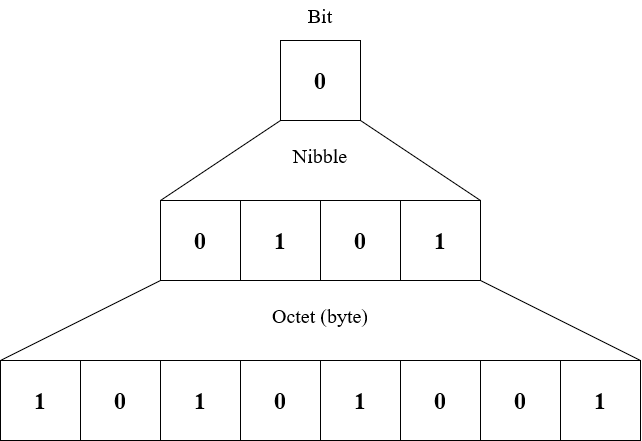
\includegraphics[width=0.5\textwidth]{byte.png}
 \centering
 \caption{Modul de împărțire a unui octet, părțile sale constituente}
 \label{Figura:1}
 \end{figure}

Octet-ul va reprezenta unitatea fundamentală și indivizibilă pentru microarhitectura microprocesorul dezvoltat prin această lucrare. Acesta, prin urmare, este cea mai mică entitate adresabilă cu care se va lucra. Un octet este limitat de numărul de date pe care le poate reprezenta, acestea fiind calculate prin exponentul $\ 2^n$, în cazul nostru, $\ 2^8$ sau 256 de valori.

Un lucru important de menționat este că valoarea maximă a unui număr pe \textit{n} biți va fi mereu $\ 2^n -1$. Prin urmare, dacă dorim să reprezentăm o putere oarecare $\ 2^n$, vor fi necesari $\ n +1$ biți de date.
Tabelul \ref{Tabela:2} prezintă realația dintre magnitudinea binară (număul de biți folosiți în reprezentare) și cantitata de date reprezentate prin plaja de valori adiacentă, ignorând existenta numerelor negative.

\begin{table}[h]
\centering
\caption{Plaja de valori asumând numere strict pozitive, de magnitudini binare diverse }
\label{Tabela:2}
\begin{tabular}{ ||c|c|c|| }
 \hline
 Biți de date & Numărul datelor & Interval valori \\ 
 \hline  \hline
 8 & 256 & $\ 0 \le n \le 2^{8} - 1$ \\
 \hline
 16 & 65536 & $\ 0 \le n \le 2^{16} - 1$ \\
 \hline
 32 &  $\ 2^{32}$ & $\ 0 \le n \le 2^{32} - 1$ \\
 \hline
 64 & $\ 2^{64}$ & $\ 0 \le n \le 2^{64} -1$ \\
 \hline
\end{tabular}
\end{table}

\subsubsection{BAZA HEXADECIMALĂ}
Datorită clarificării reprezentării datelor în radix-ul binar, întelegerea bazei hexadecimale va fi cu atât mai simplă. Convertirea unui număr din binar in hexadecimal se face pe baza împărțirii acestuia în serii de \textit{nibble}. În situația când reprezentarea binară nu are destui biți pentru a acomoda o așa diviziune a sa, se completează cu diferența de simboluri de 0 necesare. Tabela \ref{Tabela:3} prezintă valorile care vor fi utilizate în conversie cât și echivalența dintre baza binară, decimală și hexadecimală.

\begin{table}[h]
\centering
\caption{Echivalența nibble - simbol hexadecimal }
\label{Tabela:3}
\begin{tabular}{ ||c|c|c|| }
 \hline
 Nibble & Simbol & Decimal\\ 
 \hline  \hline
 0000 & 0 & 0\\
 \hline
 0001 & 1 & 1\\
 \hline
 0010 & 2 & 2\\
 \hline
 0011 &  3 & 3\\
 \hline
 0100 & 4 & 4\\
 \hline
 0101 & 5 & 5 \\
 \hline
 0110 & 6 & 6\\
 \hline
 0111 & 7 & 7\\
 \hline
 1000 & 8 & 8\\
 \hline
 1001 & 9 & 9\\
 \hline
 1010 & A & 10\\
 \hline
 1011 & B & 11\\
 \hline
 1100 & C & 12\\
 \hline
 1101 & D & 13\\
 \hline
 1110 & E & 14\\
 \hline
 1111 & F & 15\\
 \hline
\end{tabular}
\end{table}

\subsubsection{OPERAȚIILE MATEMATICE ȘI NUMERELE BINARE}
Pentru a utiliza în mod corect reprezentările în această bază, modul în care calculele matematice sunt efectuate asupra numerelor binare necesită clarificare.

Datele nu sunt folositoare doar prin existența lor. Pentru a dobândi utilitate, acestea sunt supuse aparatului matematic, prin care se calculează diverse valori, asumând un algoritm corect, care ne oferă informații despre problema pe care dorim să o rezolvăm.

Cea mai elementară operație matematică care poate fi aplicată unui număr este adunarea. Însumarea numerelor este cu atât mai facilă cu cât numărul de simboluri folosite în reprezentarea acestora scade. Spre norocul lumii digitale, radix-ul utilizat permite efectuarea operațiilor matematice în cele mai simple metode. Există doar $\ 4$ operații fundamentale posibile, acestea fiind prezentate în Tabela \ref{Tabela:3}.

\begin{table}[h]
\centering
\caption{Operațiile fundamentale de însumare a numerelor binare }
\label{Tabela:4}
\begin{tabular}{ ||c|c|c|| }
 \hline
 Operație & Sumă & Carry \\ 
 \hline  \hline
 0 + 0 & 0 & 0\\
 \hline
 0 + 1 & 1  & 0\\
 \hline
 1 + 0 &  1 & 0 \\
 \hline
 1 + 1 & 0 & 1 \\
 \hline
\end{tabular}
\end{table}
Dintre toate aceste operații, cea căreia îi vom oferi o importanță ridicată este $\ 1 + 1 = 0$ \textit{carry} 1. Aceasta  ne obligă să adunăm o unitate bițiilor de pe poziții superioare. Practic, acestă sumă, odată ce este generalizată, ne spune că $\ 2^n + 2^n = 2 \cdot 2^n = 2^{n+1}$, o trivialitate matematică. Diverse exemple de adunare ale numerelor binare pot fi consultate în Figura \ref{Figura:2}.

 \begin{figure}[h!]
 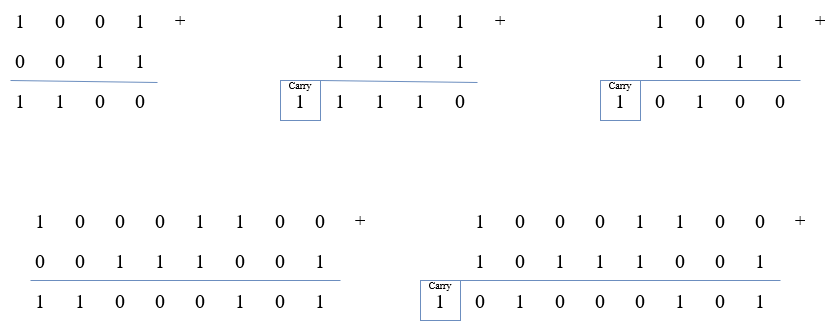
\includegraphics[width=0.9\textwidth]{binary_addition.png}
 \centering
 \caption{Exemple de adunare a numerelor binare}
 \label{Figura:2}
 \end{figure}

\subsubsection{REPREZENTAREA NUMERELOR NEGATIVE}
Modul în care numerele positive sunt adunate fiind acum clarificat, următoara operație matematică tratată este scăderea. Aceasta poate fi vizualizată ca adunarea unui numar \textit{a} la inversul aditiv al altui număr \textit{b}.
Această operație cere prin urmare un mod de reprezentare al numerelor binare negative, soluție care vine prin trei metode.

Primul mod de reprezentare este cel prin semn-magnitudine. Acesta este intuitiv, fiind similar cu reprezentarea numerelor decimale cu semn. Bit-ul cel mai semnificativ devine acum bit-ul de semn, 1 reprezentând un număr negativă, iar 0 unul pozitiv. Tabelul \ref{Tabela:4} prezintă aplicarea acestei reprezentări asupra numerelor pe 8 biți.

\begin{table}[h]
\centering
\caption{Reprezentarea prin semn-magnitudine }
\label{Tabela:5}
\begin{tabular}{ ||c|c|c|| }
 \hline
 Valoare binară & Semn magnitudine &  Fără semn\\ 
 \hline  \hline
 00000000 & 0 & 0\\
 \hline
 00000001 & 1  & 1\\
 \hline
 00000010 &  2 & 2 \\
 \hline
  ... &  ... & ... \\
 \hline
 01111110 & 126 & 126 \\
 \hline
 01111111 & 127 & 127 \\
 \hline
 10000000 & -0 & 128 \\
 \hline
 10000001 & -1 & 129 \\
 \hline
 10000010 & -2 & 130 \\
 \hline
   ... &  ... & ... \\
 \hline
  11111101 & -125 & 253 \\
 \hline
 11111110 & -126 & 254 \\
 \hline
 11111111 & -127 & 255 \\
 \hline
\end{tabular}
\end{table}
Se pot astfel distinge următoarele lucruri:
\begin{itemize}
\item Există două reprezentări posibile pentru 0, și anume $\ \pm 0$.
\item Deși se acopera tot 255 de valori numerice posibile (256 cu cel de al doilea 0), plaja de valori \textit{signed} s-a distribuit egal numerelor negative și celor pozitive. Astfel, numerele \textit{unsigned} semn-magnitudine  sunt cuprinse în intervalul $\ [-2^{n-1}+1, 2^{n-1}-1]$ unde $\ n > 0$ 
\end{itemize}

O altă medotă de reprezentare este prin complementul de 1. Conform acesteia, se inversează biții numărului binar pozitiv (biții cu valoarea 1 vor deveni 0 și viceversa) rezultând astfel inversul său aditiv. Spre exemplu, $\ 00000001' = 11111110;$ $\ 01010101' = 10101010$ iar, în cazul lui 0, $\ 00000000' = 11111111$. Tabela \ref{Tabela:5} conține reprezentările numerelor de 8 biți.
\begin{table}[h]
\centering
\caption{Reprezentarea prin complement de 1 }
\label{Tabela:6}
\begin{tabular}{ ||c|c|c|| }
 \hline
 Valoare binară & Semn magnitudine &  Fără semn\\ 
 \hline  \hline
 00000000 & 0 & 0\\
 \hline
 00000001 & 1  & 1\\
 \hline
 00000010 &  2 & 2 \\
 \hline
  ... &  ... & ... \\
 \hline
 01111110 & 126 & 126 \\
 \hline
 01111111 & 127 & 127 \\
 \hline
 10000000 & -127 & 128 \\
 \hline
 10000001 & -126 & 129 \\
 \hline
 10000010 & -125 & 130 \\
 \hline
   ... &  ... & ... \\
 \hline
  11111101 & -2 & 253 \\
 \hline
 11111110 & -1 & 254 \\
 \hline
 11111111 & -0 & 255 \\
 \hline
\end{tabular}
\end{table}

La fel ca în cazul reprezentării prin semn-magnitudine, 0 dorește să respecte principiul superpoziției, diferența pricipală însă, precum se distinge din compararea Tabelei \ref{Tabela:5} cu  Tabela \ref{Tabela:4}, este faptul ca valorile negative sunt eșalonate invers.

Problema acestor reprezentări este cu atât mai vizibilă când se efectuează adunarea a două numere binare, rezultatul fiind mereu $\ 111..1..111$, unda dintre reprezentările posibile ale lui 0. Soluția vine prin complementul de 2, complement format prin adăugarea unei unități reprezentării complementare de 1. Efectul însumării unitare este cel mai bine explicitat de Figura \ref{Figura:3}.
 
 \begin{figure}[h!]
 \[\begin{tikzcd}[cramped,column sep=tiny,row sep=scriptsize]
	& 10000000 && 11111110 & {00000000 = 11111111} & 00000001 && 01111111 \\
	& {-127} & {...} & {-1} & 0 & 1 & {...} & 127 \\
	\\
	10000000 & 10000000 && 11111111 & 00000000 & 00000001 && 01111111 \\
	{-128} & {-127} & {...} & {-1} & 0 & 1 & {...} & 127
	\arrow["{+1}"{description}, from=2-2, to=4-2]
	\arrow[from=2-3, to=2-2]
	\arrow[from=2-4, to=2-3]
	\arrow["{+1}"{description}, from=2-4, to=4-4]
	\arrow[from=2-5, to=2-4]
	\arrow[from=2-5, to=2-6]
	\arrow[from=2-6, to=2-7]
	\arrow[from=2-7, to=2-8]
	\arrow[from=4-2, to=5-2]
	\arrow[from=4-4, to=5-4]
	\arrow[from=5-2, to=5-1]
	\arrow[from=5-3, to=5-2]
	\arrow[from=5-4, to=5-3]
	\arrow[from=5-5, to=5-4]
	\arrow[from=5-5, to=5-6]
	\arrow[from=5-6, to=5-7]
	\arrow[from=5-7, to=5-8]
\end{tikzcd}\]
 \centering
 \caption{Efectul adunării unității asupra complementului de 1}
 \label{Figura:3}
% https://q.uiver.app/#q=WzAsMjYsWzQsMCwiMDAwMDAwMDAgPSAxMTExMTExMSJdLFs0LDEsIjAiXSxbNCw0LCIwIl0sWzQsMywiMDAwMDAwMDAiXSxbMiw0LCIuLi4iXSxbMiwxLCIuLi4iXSxbNiwxLCIuLi4iXSxbNiw0LCIuLi4iXSxbMCw0LCItMTI4Il0sWzMsNCwiLTEiXSxbNSw0LCIxIl0sWzUsMywiMDAwMDAwMDEiXSxbNyw0LCIxMjciXSxbNywzLCIwMTExMTExMSJdLFs1LDEsIjEiXSxbNSwwLCIwMDAwMDAwMSJdLFs3LDEsIjEyNyJdLFs3LDAsIjAxMTExMTExIl0sWzMsMSwiLTEiXSxbMywwLCIxMTExMTExMCJdLFszLDMsIjExMTExMTExIl0sWzEsMSwiLTEyNyJdLFsxLDQsIi0xMjciXSxbMSwwLCIxMDAwMDAwMCJdLFsxLDMsIjEwMDAwMDAwIl0sWzAsMywiMTAwMDAwMDAiXSxbMiw5XSxbMiwxMF0sWzEwLDddLFs3LDEyXSxbMSwxNF0sWzE0LDZdLFs2LDE2XSxbMSwxOF0sWzE4LDIwLCIrMSIsMV0sWzIwLDldLFsxOCw1XSxbOSw0XSxbNSwyMV0sWzQsMjJdLFsyMiw4XSxbMjEsMjQsIisxIiwxXSxbMjQsMjJdXQ==

\end{figure}

\newpage
Din această figură se observa următoarele:
\begin{itemize}
\item În cazul complementului de 2, nu mai există două reprezentări posibile pentru 0, locul suplimentar fiind luat de posibilitatea reprezentării unui număr negativ adițional, $\ -128$.
\item Intervalul posibil de valori devine acum  $\ [-2^{n-1}, 2^{n-1}-1]$.
\end{itemize}

Odată cu clarificarea reprezentării numerelor binare negative, operațiile matematice fundamentale pe care microprocesorul modelat pe decursul acestei lucrări le va utiliza, pot fi acum implementate. Însă, pentru a face legătura dintre abstractul arhitectural al sistemului și datele numerice, este necesară tratarea entităților digitale fundamentale cunoscute drept porți logice. 

\subsection{ABSTRACȚIA LOGICĂ} 

Porțile logice sunt acele dispozitive care fac legătura dintre operațiile matematice abstracte definite anterior și implementarea propriu zisă a sistemului practic de calcul. În spatele unei porți logice se găsesc tranzistoarele, mici întrerupătoare electrice ale căror mărime a ajuns în zilele noastre să atingă ordinul nanometric (\textit{$\ 10^{-9}$ metri}). Subtilitățile de  funcționare ale unui tranzistor sunt dincolo de scopul acestei lucrări, acesta fiind considerat cutia neagră de la baza implementării entităților digitale.

O poartă logică are rolul de a implementa o funcție matematică a algebrei Booleane. Comportamentul acestora este considerat ideal, întârzierile de propagare a impulsului astfel neglijabile. Pentru analiza funcției algebrice descrise se vor utiliza  tabele logice,a căror rol este de a relaționa în format tabelar semnalele de intrare cu rezultatul produs.

Un amalgam de porți logice cumulat după operația definită de o funcție algebrică formează un sistem logic de o complexitate variată. Printre acestea se număra dispozitivele de memorare, de la \textit{flip-flop-uri} și \textit{bistabile} la \textit{RAM} și \textit{ROM}, dar și cele aritmetice precum \textit{ALU} (unitatea aritmetică logică) și \textit{FPU} (coprocesorul pentru numere cu virgulă flotantă).


\subsubsection{BUFFER}
Un buffer reprezintă cea mai simplă poartă logică. Rolul acesteia este de a transmite exact semnalul pe care-l primește ca intrare, adaugând însă o întârziere de propagare. Simbolul porții logice este prezentat de Figura \ref{Figura:4}.

 \begin{figure}[h!]
\begin{tikzpicture}[thick,scale=2.0, every node/.style={transform shape}]
    \node (x) at (0, 1) {$A$};
    \node (y) at (1.9, 1) {$Q$};
    \node[buffer gate US, draw] at ($(x) + (0.8, 0)$) (notx) {};
    \draw (x) -- (notx.input);
    \draw (notx.output) -- ++(0.4, 0);
\end{tikzpicture}
 \centering
 \caption{Simbolul porții logice Buffer}
 \label{Figura:4}
\end{figure}
 
 Utilitatea acesteia se poate observa în special la nivelul procesoarelor  multi-cycle, buffer-ul având un rol important în organizarea modului de execuție a instrucțiunilor complexe care necesită multiple cicluri de tact. 
 
\subsubsection{NOT}
De asemenea cunoscut sub numele de \textit{inversor}, rolul acestei porți logice este 
de a schimba polaritatea semnalului primit.
 
 \begin{table}[h]
\centering
\caption{Funcția logică NOT}
\label{Tabela:7}
\begin{tabular}{ ||c|c|| }
 \hline
 A & Q\\ 
 \hline  \hline
 1 & 0 \\
 \hline
 0 & 1 \\
 \hline
\end{tabular}
\end{table}

Tabela \ref{Tabela:7} prezintă functionalitatea acestei porți. Simbolul utilizat în diagramele circuitelor este prezentat prin Figura \ref{Figura:5}. Ecuația matematică a inversorului este $\ Q = \overline{A}$.


 \begin{figure}[h!]
\begin{tikzpicture}[thick,scale=2.0, every node/.style={transform shape}]
    \node (x) at (0, 1) {$A$};
    \node (y) at (1.9, 1) {$Q$};
    \node[not gate US, draw] at ($(x) + (0.8, 0)$) (notx) {};
    \draw (x) -- (notx.input);
    \draw (notx.output) -- ++(0.4, 0);
\end{tikzpicture}
 \centering
 \caption{Simbolul porții logice NOT}
 \label{Figura:5}
\end{figure}
 
\subsubsection{SAU}
Poarta logică \textit{sau} reprezintă implementarea operației de disjuncție matematică, a cărei rezultat este 0 doar atunci când ambele intrări logice sunt 0. Tabela \ref{Tabela:8} prezintă valorile operației raportate la intrările logice. Expresia matematică a operației \textit{sau} este $\ Q = A+B$.
 \begin{table}[h]
\centering
\caption{Funcția logică SAU}
\label{Tabela:8}
\begin{tabular}{ ||c|c|c|| }
 \hline
 A & B & Q\\ 
 \hline  \hline
 1 & 1 & 1 \\
 \hline
 1 & 0 & 1 \\
 \hline
 0 & 1 & 1 \\
 \hline 
 0 & 0 & 0 \\
 \hline
\end{tabular}
\end{table}

Simbolul utilizat în diagramele circuitelor este prezentat prin Figura \ref{Figura:6}.

 \begin{figure}[h!]
    \begin{tikzpicture}[thick,scale=1.3, every node/.style={transform shape}]
    \node[or gate US, minimum size = 28pt, draw] at (1.5,0.5) (NAND) {};
	\node[label={[above] left:$A$}] at ([xshift=-0.6cm]NAND.input 1) (A) {};
	\node[label={[below] left:$B$}] at ([xshift=-0.6cm]NAND.input 2) (B) {};
	\draw (A.east) -- (NAND.input 1);
	\draw (B.east) -- (NAND.input 2);
    \draw (NAND.output) -- ($(NAND) + (1.2,0)$);
    \node (z) at ($(NAND) + (1.5,0)$) {$Q$};
    \end{tikzpicture}
 \centering
 \caption{Simbolul porții logice SAU}
 \label{Figura:6}
 \end{figure}
 
\subsubsection{ȘI}
Poarta logică \textit{și} reprezintă implementarea operației de conjuncție matematică, a cărei rezultat este 1 doar atunci când ambele intrări logice sunt 1. Tabela \ref{Tabela:9} prezintă valorile operației raportate la intrările logice. Expresia matematică a operației \textit{și} este $\ Q = A \cdot B$.
 \begin{table}[h]
\centering
\caption{Funcția logică ȘI}
\label{Tabela:9}
\begin{tabular}{ ||c|c|c|| }
 \hline
 A & B & Q\\ 
 \hline  \hline
 1 & 1 & 1 \\
 \hline
 1 & 0 & 0 \\
 \hline
 0 & 1 & 0 \\
 \hline 
 0 & 0 & 0 \\
 \hline
\end{tabular}
\end{table}

\newpage
Simbolul utilizat în diagramele circuitelor este prezentat prin Figura \ref{Figura:7}.

 \begin{figure}[h!]
    \begin{tikzpicture}[thick,scale=1.3, every node/.style={transform shape}]
    \node[and gate US, minimum size = 28pt, draw] at (1.5,0.5) (NAND) {};
	\node[label={[above] left:$A$}] at ([xshift=-0.6cm]NAND.input 1) (A) {};
	\node[label={[below] left:$B$}] at ([xshift=-0.6cm]NAND.input 2) (B) {};
	\draw (A.east) -- (NAND.input 1);
	\draw (B.east) -- (NAND.input 2);
    \draw (NAND.output) -- ($(NAND) + (1.2,0)$);
    \node (z) at ($(NAND) + (1.5,0)$) {$Q$};
    \end{tikzpicture}
 \centering
 \caption{Simbolul porții logice ȘI}
 \label{Figura:7}
 \end{figure}

\subsubsection{XOR}
Poarta logică \textit{xor}, de asemenea cunoscută ca \textit{SAU exclusiv} setează semnalul de output pe 1 logic doar în cazul în care cel mult una dintre intrări este activă. Comportamentul acesteia este cel mai bine reprezentat de Tabela \ref{Tabela:10}. Expresia matematică care descrie această poartă este $\ Q = A \oplus B$.
\begin{table}[h]
\centering
\caption{Funcția logică XOR}
\label{Tabela:10}
\begin{tabular}{ ||c|c|c|| }
 \hline
 A & B & Q\\ 
 \hline  \hline
 1 & 1 & 0 \\
 \hline
 1 & 0 & 1 \\
 \hline
 0 & 1 & 1 \\
 \hline 
 0 & 0 & 0 \\
 \hline
\end{tabular}
\end{table}


Această operație logică implică practic excluderea mutuală a semnalelor de intrare, indiferent de numărul acestora. Simbolul logic utilizat în diagramele digitale se poate regăsi în Figura \ref{Figura:8}.
 \begin{figure}[h!]
    \begin{tikzpicture}[thick,scale=1.3, every node/.style={transform shape}]
    \node[xor gate US, minimum size = 28pt, draw] at (1.5,0.5) (NAND) {};
	\node[label={[above] left:$A$}] at ([xshift=-0.6cm]NAND.input 1) (A) {};
	\node[label={[below] left:$B$}] at ([xshift=-0.6cm]NAND.input 2) (B) {};
	\draw (A.east) -- (NAND.input 1);
	\draw (B.east) -- (NAND.input 2);
    \draw (NAND.output) -- ($(NAND) + (1.2,0)$);
    \node (z) at ($(NAND) + (1.5,0)$) {$Q$};
    \end{tikzpicture}
 \centering
 \caption{Simbolul porții logice XOR}
  \label{Figura:8}
 \end{figure}

\newpage
\subsubsection{NAND}
Ca o regulă generala, totalitatea porților logice la ale căror denumire se atașează prefixul \textit{N-} sunt varianta negată a portii logice originale. Însă, spre deosebire de restul porților, NAND este de asemenea cunoscută ca și poarta logică fundamentală. Această denumire reiese din operațiile algebrei Booleane.

 În mod firesc, semnalul de ieșire al acestei porți va fi complementarul operației \textit{and}. La nivelul Tabelei \ref{Tabela:11} se poate observa acest lucru. Expresia matematică a acestei operații este  $\ Q = \overline{A \cdot B}$.
 \begin{table}[h]
\centering
\caption{Funcția logică NAND}
\label{Tabela:11}
\begin{tabular}{ ||c|c|c|| }
 \hline
 A & B & Q\\ 
 \hline  \hline
 1 & 1 & 0 \\
 \hline
 1 & 0 & 1 \\
 \hline
 0 & 1 & 1 \\
 \hline 
 0 & 0 & 1 \\
 \hline
\end{tabular}
\end{table}

Simbolul utilizat în diagramele circuitelor este prezentat prin Figura \ref{Figura:9}.
 \begin{figure}[h!]
    \begin{tikzpicture}[thick,scale=1.3, every node/.style={transform shape}]
    \node[nand gate US, minimum size = 28pt, draw] at (1.5,0.5) (NAND) {};
	\node[label={[above] left:$A$}] at ([xshift=-0.6cm]NAND.input 1) (A) {};
	\node[label={[below] left:$B$}] at ([xshift=-0.6cm]NAND.input 2) (B) {};
	\draw (A.east) -- (NAND.input 1);
	\draw (B.east) -- (NAND.input 2);
    \draw (NAND.output) -- ($(NAND) + (1.2,0)$);
    \node (z) at ($(NAND) + (1.5,0)$) {$Q$};
    \end{tikzpicture}
 \centering
 \caption{Simbolul porții logice NAND}
 \label{Figura:9}
 \end{figure}
 
\subsubsection{MULTIPLEXARE}
Pe lângă circuitele clasice reprezentate de porțile logice, un alt component digital, multiplexorul, merită studiat, acesta având o importanță deosebită. Prin multiplexare se întelege selecția unui anumite intrări dintr-o lista de \textit{n} posibilități. Selecția este dictată de un alt semnal de intrare numit selecție sau selector.

Multiplexara de asemenea are o operație opusă, aceasta purtând numele de demultiplexare. Dintr-o listă de \textit{n} ieșiri posibile, se va alege conform semnalului selector drumul pe care-l va lua un semnal de intrare.

Atunci când se dorește utilizarea unui dispozitiv multiplexor, cel mai important parametru este reprezentat de numărul de intrări specificate de cazul de utilizare. Conform acestor \textit{n} intrări, se va calcula utilizând expresia $\log_2{n}$ biții necesari semnalului de selecție.

Figura \ref{Figura:24} arată modul de reprezentare grafic al unui multiplexor cu 4 intrări pe 32 de biți și un semnal de selecție de 2 biți.
 \begin{figure}[h]
 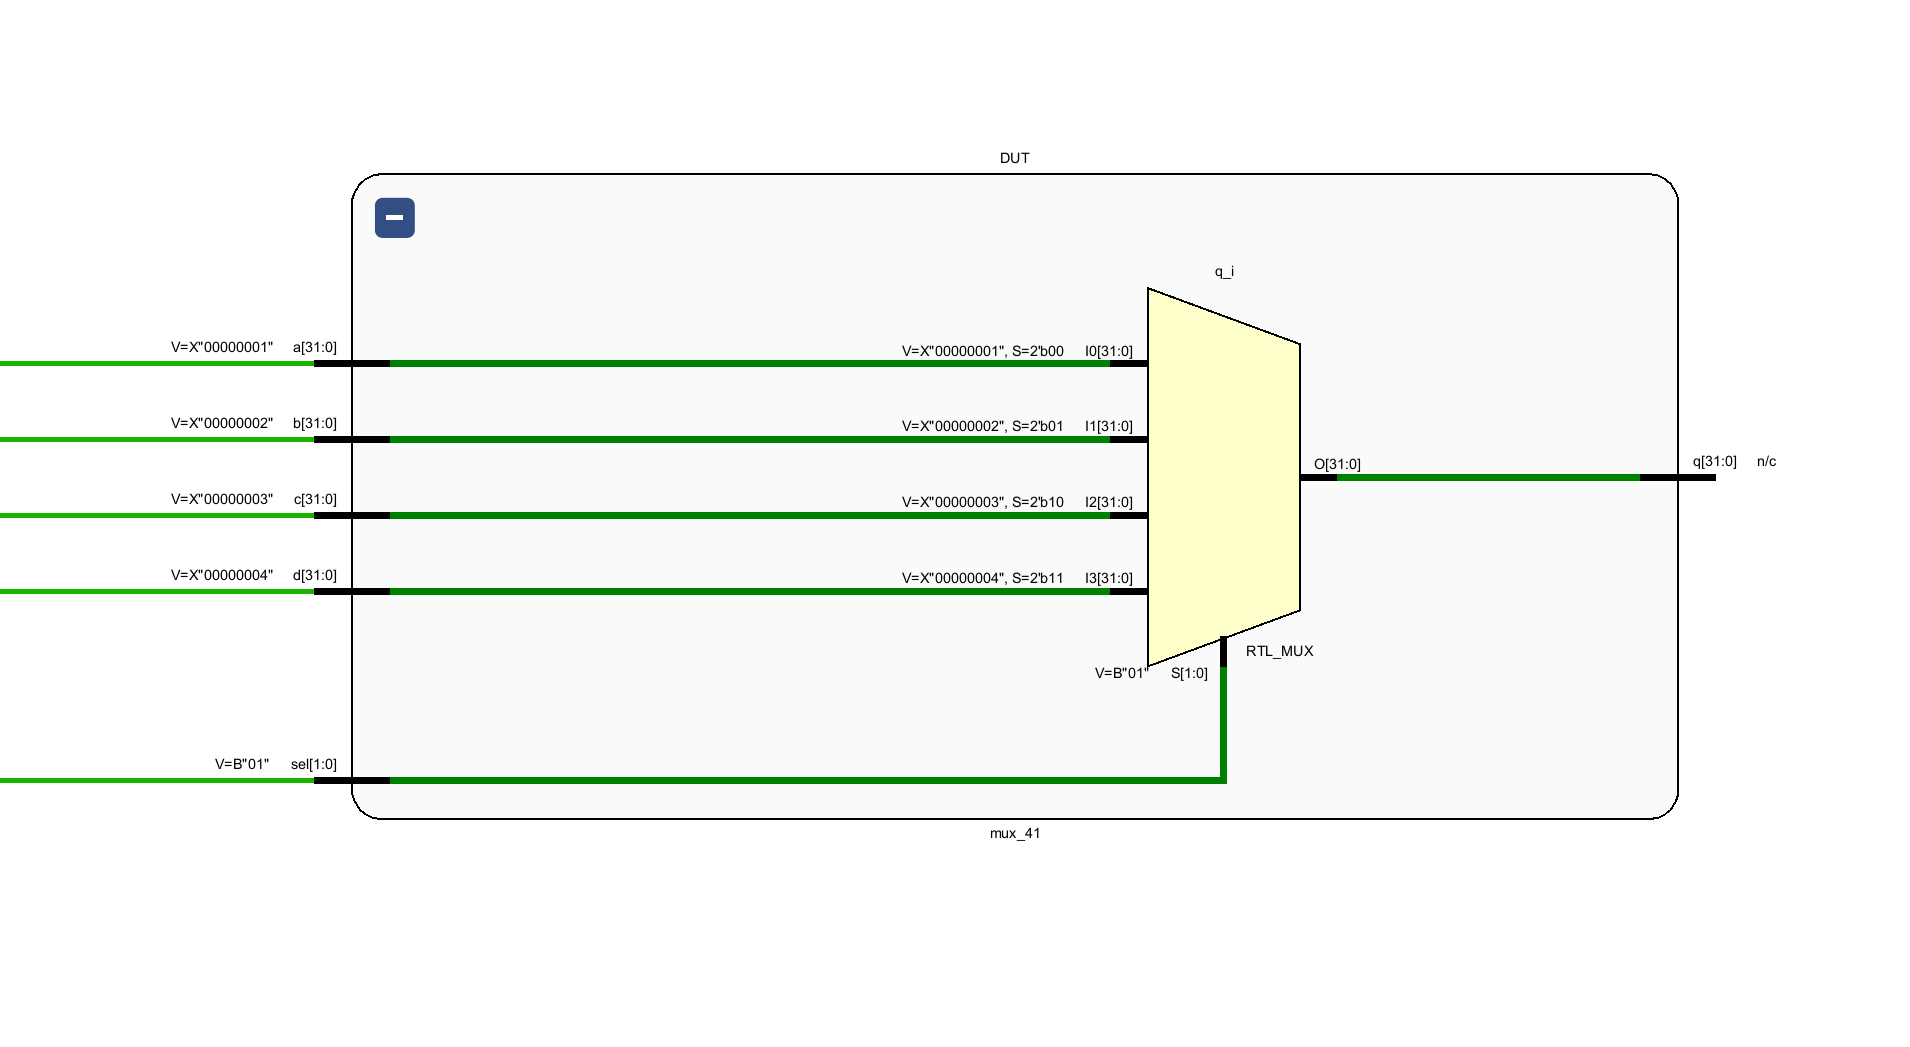
\includegraphics[width=0.5\textwidth]{mux41.png}
 \centering
 \caption{Diagrama logică a unui multiplexor}
 \label{Figura:24}
 \end{figure}
 

\newpage
 \subsection{ABSTRACTIA ARHITECTURALĂ}
Arhitectura face legătura dintre microarhitectura sistemului și programatorul care dorește să-l utilizeze. Acest nivel de abstracție are rolul de a oferi un ghid asupra interacțiunii cu interfața definită de standardul RISC-V. Prin urmare, vor analiza detalile arhitecturii, printre care se numără structura organizațională a registrelor, tipurile de instrucțiuni cât si modul în care octeții sunt organizați la nivelul acestora. Ne vom limita însă la extensia de bază RISC-V care include doar instrucțiunile fundamentale asupra numerelor întregi.

\subsubsection{FIȘIERUL DE REGISTRE}
  Cel mai important detaliu microarhitectural este fișierul de registre. Acesta este singurul dintre elementele de design a cărei respectare a tiparului impus de standardul RISC-V este imperativă.
  
   Standardul impune un fișiser de 32 de registre în cazul setului RV32I și 32 sau 64 de registre, în funcție de mărimea spațiului de adresare, pentru un procesor RV64I. Denumirea acestor registre, conform convenției, îndică modul destinat de utilizare dar, nu există constrângeri la doar astfel de utilizări.
   
Tabela \ref{Tabela:12} ne ajută să identificăm registrele procesorului RV32I cât și utilizarea acestora. Coloana \textit{Denumire Simbolică} prezintă modul de adresarea ale acestor registre la nivelul limbajului de asamblare.

\begin{table}[h]
\centering
\caption{Fișierul de registre RV32I}
\label{Tabela:12}
\begin{tabular}{ ||c|c|c|| }
 \hline
 Registru & Denumire simbolică & Descriere\\ 
 \hline  \hline
 x0 & zero & Legat la valoarea 0 \\
 \hline
 x1 & ra & Adresa de return \\
 \hline
 x2 & sp & Pointer stivă \\
 \hline 
 x3 & gp & Pointer global \\
  \hline
 x4 & tp & Pointer thread \\
  \hline  
 x5-7 & t0-2 & Valori temporare \\
 \hline
 x8 & fp & Stocare date sau pointer cadru \\
  \hline  
 x9 & s1 & Stocare date \\
  \hline  
 x10-11 & a0-1 & Argumente apel funcție sau valori de return \\
  \hline  
 x12-17 & a2-7 & Argumente apel funcție \\
  \hline  
 x18-27 & s2-11 & Stocare date \\
  \hline  
 x28-31 & t3-6 & Valori temporare \\
  \hline  
\end{tabular}
\end{table}

\subsubsection{INSTRUCȚIUNILE DE BAZĂ RISC-V}

Operațile de bază executate de un procesor RV32I sunt transcrise în instrucțiuni având o mărime de 4 octeți. Aceste instrucțiuni pot fi de următoarele tipuri:

\begin{itemize}
\item Instrucțiuni R, \textit{Register-Register}, pentru operațile de la registru la registru.
\item Instrucțiuni I, \textit{Immediate}, pentru operații asupra valorilor imediate.
\item Instrucțiuni S, \textit{Store}, cu rol de încărcare a datelor în memoria volatilă.
\item Instrucțiuni U, \textit{Upper Immediate}, cu rol de încarcare imediată a octeților cei mai semnificativi în registre.
\end{itemize}

În cazul instrucțiunilor care utilizează valori imediate este importat să se țină cont de lătimea acestor valori. Familia de instrucțiuni U permite o lătime mai ridicată acestor tip de valori decât lătimea permisă de familia I.

\subsubsection{INSTRUCȚIUNEA R}
Instrucțiunile de acest format adresează 3 registre, 2 dintre ele fiind sursa datelor, cel de al 3-lea reprezentând destinația. Acestea sunt în general utilizate în operațile aritmetice, precum adunarea și scăderea numerelor. Figura \ref{Figura:10} prezintă formatul acestei instrucțiuni cât și câmpurile de date constituente.



 \begin{figure}[h!]
 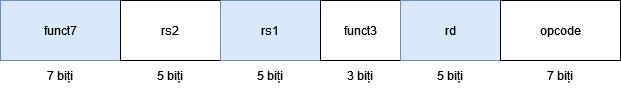
\includegraphics[width=0.6\textwidth]{rtype.drawio.png}
 \centering
 \caption{Instrucțiunea R și câmpurile de date}
 \label{Figura:10}
 \end{figure}

 Campurile acestei instrucțiuni au următoarele semnificații:
 \begin{itemize}
\item Câmpul \textit{opcode} indică tipul instrucțiinii care va fi executată de ALU.
\item Câmpul \textit{rd} conține adresa registrului unde va fi stocat rezultatul operației.
\item Câmpul \textit{rs1} conține adresa registrului primului operand.
\item Câmpul \textit{rs2} conține adresa registrului celui de al 2-lea operand.
\item Câmpurile \textit{funct7} și \textit{funct3} conțin date adiționale pentru operația aritmetică de executat.
\end{itemize}

Un exemplu practic al acestei instrucțiuni se poate vedea în Figura \ref{Figura:11}. Datele din registrele 1 și 2 sunt însumate, rezultatul fiind plasat în registrul 3. De menționat faptul că trebuie acordată atenție sporită câmpurilor de specificare a operației de executat.
\newpage
 \begin{figure}[h!]
 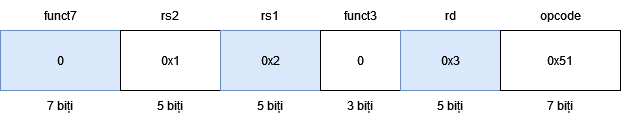
\includegraphics[width=0.6\textwidth]{rtypeexample.png}
 \centering
 \caption{Exemplu de utilizare al instrucțiunii R}
 \label{Figura:11}
 \end{figure}

\subsubsection{INSTRUCȚIUNEA S}
Rolul instrucțiunilor de acest format este stocarea datelor. Pentru a facilita acest lucru, formatul instrucțiunii include 2 registre și câmpul imediat. Un registru este utilizat în calculul adresei de memorie, alături de un offset reprezentat de datele imediate, cel doilea conținând datele care se doresc stocate. Figura \ref{Figura:12} arată structura unei astfel de instrucțiuni.
 \begin{figure}[h!]
 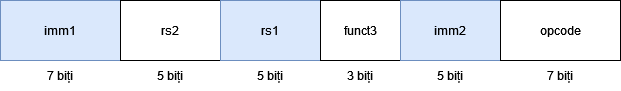
\includegraphics[width=0.6\textwidth]{stype.png}
 \centering
 \caption{Instrucțiunea S și câmpurile de date}
 \label{Figura:12}
 \end{figure}
 
Semnificația câmpurilor este următoarea:
 \begin{itemize}
\item Câmpul \textit{opcode} indică tipul instrucțiinii de executat.
\item Câmpul \textit{rs1} conține adresa registrului în care se găsesc datele destinate stocării.
\item Câmpul \textit{rs2} conține adresa registrului față de a cărui valoare se va calcula offset-ul.
\item Câmpul \textit{funct3} conțin date adiționale despre operația de \textit{store} executată.
\item Câmpul \textit{Immediate} format din \textit{imm1} și \textit{imm2}, în această ordine,  reprezintă offset-ul adresei în care de dorește stocarea.
\end{itemize}


Un exemplu practic al acestei instrucțiuni se poate vedea în Figura \ref{Figura:13}. Valoarea din registrul 1 va fi stocată la adresa indicată de registrul 2, la care se va adauga un offset de \textit{-1}.

 \begin{figure}[h!]
 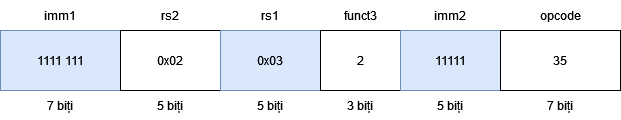
\includegraphics[width=0.6\textwidth]{stypeexample.png}
 \centering
 \caption{Exemplu de utilizare al instrucțiunii S}
 \label{Figura:13}
 \end{figure}
 
 \subsubsection{INSTRUCȚIUNEA I}
 Instrucțiunea I are rol în execuția operaților aritmetice cu valori imediate. Aceste valori sunt extinse la 32 de biti, ele ocupând doar 12 biți din lătimea instrucțiunii. În urma extensiei de semn, se efectueaza operația aritmetică specificată prin câmpul \textit{funct3} cu registrul \textit{rs1}, rezultatul fiind stocat în registrul \textit{rd}. Figura \ref{Figura:14} prezintă structura instrucțiunii și câmpurile relevante.

 \begin{figure}[h!]
 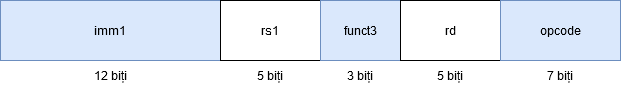
\includegraphics[width=0.6\textwidth]{itype.png}
 \centering
 \caption{Instrucțiunea I și câmpurile de date}
 \label{Figura:14}
 \end{figure}

 Fie o valoare imediată egală cu \textit{5}, se dorește însumarea sa cu valoare din registrul \textit{1}, rezultatul operației fiind trimis registrului \textit{3}. Un astfel de exemplu se poate vedea în Figura \ref{Figura:15}.

 \begin{figure}[h!]
 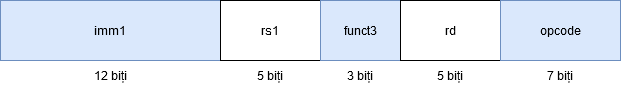
\includegraphics[width=0.6\textwidth]{itype.png}
 \centering
 \caption{Instrucțiunea I și câmpurile de date}
 \label{Figura:15}
 \end{figure}
 
 \subsubsection{INSTRUCȚIUNEA U}
 Această instrucțiune este folositoare atunci când se dorește de către programator încărcarea unei valori imediate într-un registru, vizată ulterior unor calcule. Formatul instrucțiunii are în compoziția sa câmpul datelor imediate, întins pe 20 de biți, registrul destinație și codul identificator al operației de executat.
 
  Cei 20 de biți sunt cei mai semnificativi ai numărului imediat, urmând ca acesta să fie extins la 32 de biți. Aranjamentul anterior descris poate fi observat în Figura \ref{Figura:22}.
 \begin{figure}[h!]
 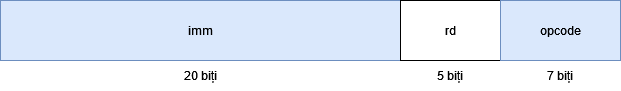
\includegraphics[width=0.6\textwidth]{utype.png}
 \centering
 \caption{Instrucțiunea U și câmpurile de date}
 \label{Figura:22}
 \end{figure}

Figura \ref{Figura:23} prezintă un exemplu de utilizare, în registrul 5 fiind încărcată valoarea imediată 0X51AA3.

 \begin{figure}[h!]
 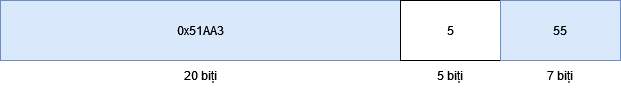
\includegraphics[width=0.6\textwidth]{utypeexample.png}
 \centering
 \caption{Exemplu de utilizare al instrucțiunii U}
 \label{Figura:23}
 \end{figure}

\newpage
\subsubsection{MEMORIA CACHE}

Procesoarele prezintă o mare ineficiență când vine vorba de execuția instrucțiunilor care lucrează cu datele din memoria principală. Această ineficiență provine din diferența dintre timpul de execuție operațional al procesorului și timpul de acces din memoria pricipală la datele necesare calculului. Diferența dintre aceste două metrici temporale poartă numele de \textit{latență}. Într-adevăr, avansurile tehnologice aduse componentelor digitale de-a lungul decenilor au ajutat minimizarea aceste latențe, însă nu destul încât să o elimine din procesul de optimizare a pipeline-ului de execuție.

Astfel, prezența latenței ne conduce la analizarea a două mari problematici în modul de lucru cu date, și anume, problemele localizării temporale și a localizării spațiale. Localitatea spațilă a datelor indică faptul ca există o mare posibilitate ca procesorul să dorească accesul unor adrese de memorie apropiate, de exemplu în cazul unei structuri de date vectoriale sau matriciale. Localizarea temporală pe de altă parte exemplifică posibilitatea accesului aceleiași adrese de memorie într-un interval de timp \textit{t}.

Fie secvența de instrucțiuni RISC-V de acces a datelor din memoria principală prezentată în Figura 19. Se poate observa faptul că procesorul dorește accesul a mai multe spații de adresare consecutive. De fiecare dată când se extrag datele din aceste adrese, unitatea de execuție este obligată să aștepte conform unui timp \textit{$\ {\Delta}$t} egal cu latența de acces a memoriei principale.

 \begin{figure}[h!]
 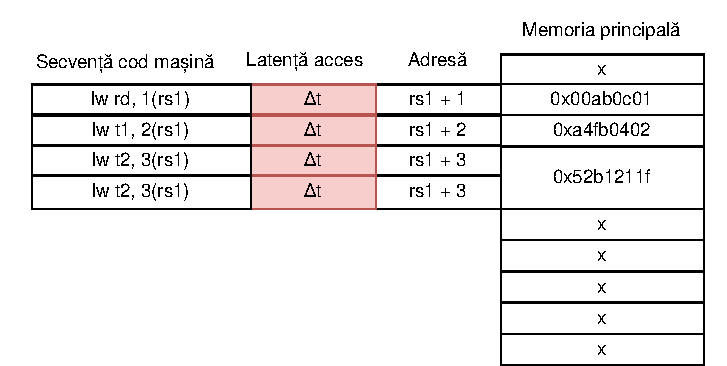
\includegraphics[width=0.8\textwidth]{cachememoryacces.pdf}
 \centering
 \caption{Accesul la memorie și latența în cazul operației lw}
 \label{Figura:40}
 \end{figure}
 
Timpul total pe care procesorul îl are de așteptat este egal cu suma timpilor de acces al memoriei principale dintr-un interval de timp discret \textit{t} în care sunt executate astfel de operații. Expresia matematică care se regăsește în Formula 2 prezintă un astfel de calcul al latenței totale, \textit{Lt}, dintr-un interval de timp $\ [1, t] $.
 
 \begin{equation}
\label{Formula:1}
Lt = \sum_{n=1}^{t} \Delta n
\end{equation}

Latența de acces, în cazul unui procesor simplificat, implică ca urmare un timp de așteptare în care execuția procesorului este practic blocată, miscorând drastic eficiența. Însă, din acest exemplu, se pot de asemenea observa principile localității anterior menționate. Procesorul accesează iterativ 3 zone de memorie alăturate, ultima fiind accesată de 2 ori, conformându-se principiului temporal.

Soluția micșorării acestei latențe vine sub forma unei memorii secundare bazate pe registre, aceasta purtând numele de \textit{memorie cache}. Din cauza costurilor ridicate de implementare, dar și a amprentei ridicate asupra spațiului ocupat pe suprafața litografiată a procesorului, memoria cache are ca regulă generală o mărime limitată.

Există mai multe arhitecturi de implementare ale unei astfel de memorii, complexitatea digitală variind drastic. Diferența arhitecturală reiese din modul de asociere a adreselor din memoria principală cu spațiul de adresare a memoriei cache. Astfel, se disting memorii cache asociative direct, asociative pe seturi și nu în ultimul rând, asociative totale.

Metoda de asociere prezentată și implementată în această lucrare este cea asociativă directă, fiind de complexitatea cea mai redusă, prin comparație cu alternativele anterior menționate. Nu trebuie însă trecută cu vederea similaritatea cu celălalte tipuri de asocieri, hardware-ul fiind similar, tot similare fiind și metodele de calcul care vor fundamenta implementarea.

Cea mai importantă caracteristică a unei astfel de memorii este mărimea sa cât și lungimea în octeți a blocurilor care o compun. Figura \ref{Figura:41} exemplifică aspectul unei memorii cache de 32 de octeți, aceștia fiind împărțiți în blocuri de câte 4 octeți. Prin urmare, fiecare bloc reține 4 cuvinte de câte un octet. Blocurile 0, 3 și 5 sunt încărcate cu date.

 Este important de menționat faptul ca un bloc trebuie să acopere la cel mai rudimentar nivel cel putin 2 adrese ale memoriei principale. Astfel, mărimea blocurilor este direct relaționată la mărimea memoriei de date, un bloc de cache acoperind \textit{n} adrese din aceasta.

 \begin{figure}[h!]
 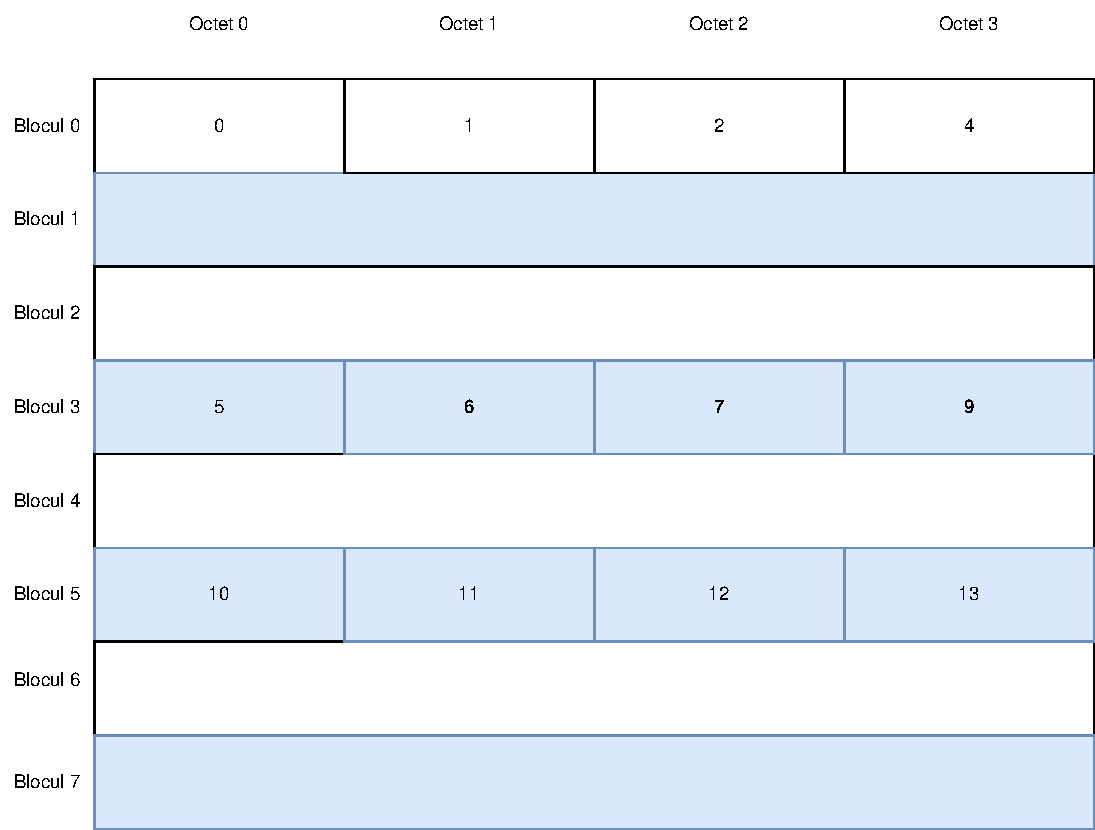
\includegraphics[width=0.65\textwidth]{cache.pdf}
 \centering
 \caption{Arhitectura memoriei de date a cache-ului}
 \label{Figura:41}
 \end{figure}
 
Memoria principală este relaționată ca și mărime a cuvântului utilizat direct cache-ului. Prin urmare, plecând de la o memoria cache cu un cuvânt de 8 biți, prezentată în Figura \ref{Figura:41}, memoria de date va avea mărimea unei adrese egală cu un octet și o mărime totală complet arbitrară, fie aceasta 1KB. Cache-ul luat ca exemplu, acoperă prin urmare un bloc de 4 adrese. Figura \ref{Figura:42} prezintă organizarea memoriei principale descrise anterior. Adresa  memoriei va avea  $\  log_2 1024 = 10$ biți.

 \begin{figure}[h!]
 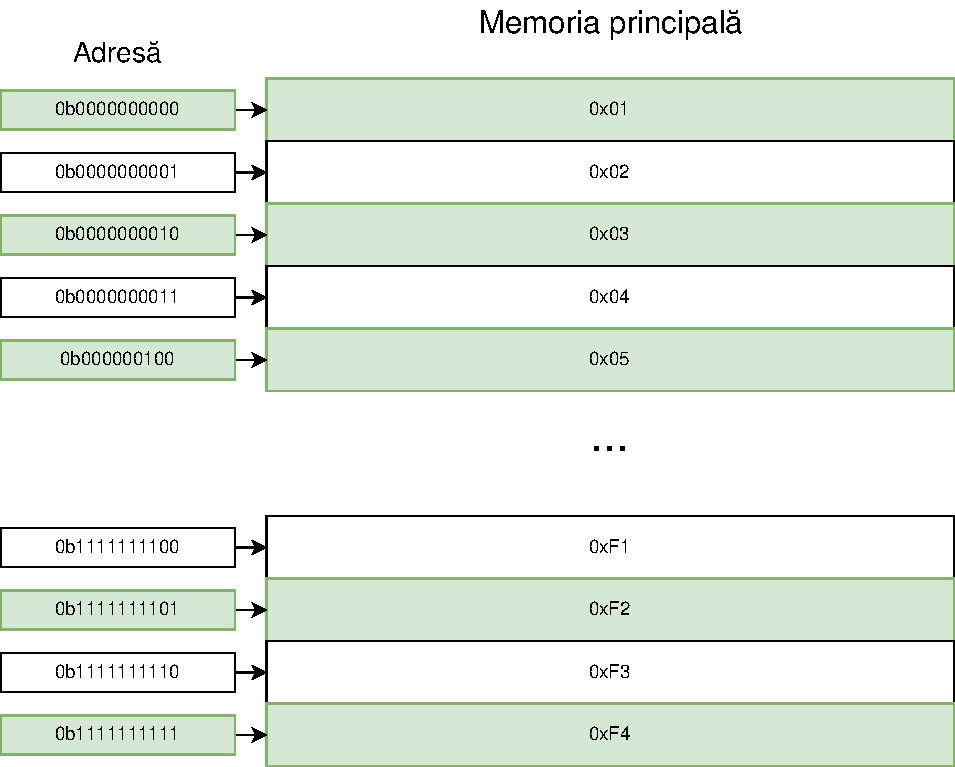
\includegraphics[width=0.6\textwidth]{mainmem2.pdf}
 \centering
 \caption{Organizarea memoriei principale}
 \label{Figura:42}
 \end{figure}
 
 
Pentru a reține datele eficient în cache, avem nevoie de un câmp de date din adresa memoriei principale care să ne semnifice blocul în care ne aflăm. Numărul de blocuri ale memoriei cache fiind egal cu 8, vor fi necesari $\  log_2 8 = 3 $ biți numiți index. Ca și o regulă generală, pentru o memorie cache cu n blocuri, vor fi necesari $\  log_2 n $ biți.

 De asemenea, pentru a relaționa fiecare adresă cu octetul din bloc în care aceasta trebuie depusă, avem nevoie de $\  log_2 4 = 2 $ biți numiți offset, 4 fiind mărimea blocului din cache. Astfel, din adresa de 10 biți, 5 vor fi folosiți pentru a ne orienta dupa blocul în care ne aflăm. Restul de 5 sunt cunoscuți drept tag și vor fi utilizați pentru a identifica unic un set de 8 blocuri (32 de octeți). Figura \ref{Figura:44} prezintă modul în care memoria a fost împărțită.

 \begin{figure}[h!]
 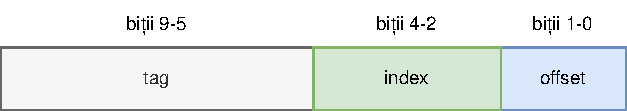
\includegraphics[width=0.7\textwidth]{memdivision.pdf}
 \centering
 \caption{Organizarea memoriei principale}
 \label{Figura:44}
 \end{figure}
 
Combinația de tag și index reprezintă practic identificatorul unic al unui bloc din memoria principală, precum este acesta relaționat la nivelul cache-ului. Datorită importanței pe care o posedă câmpul tag, acesta va fi stocat într-o memorie SRAM a cărei număr de coloane este egal cu numărul de blocuri din cache. Prezența unui anumit tag la index-ul \textit{i} din această memorie SRAM, denumită \textit{TAG SRAM}, indică existența în cache a blocului identificat prin indexul și tag-ul respectiv și a tuturor celor 4 octeți din acesta. Figura \ref{Figura:43} arată arhitectura memoriei TAG SRAM.

 \begin{figure}[h!]
 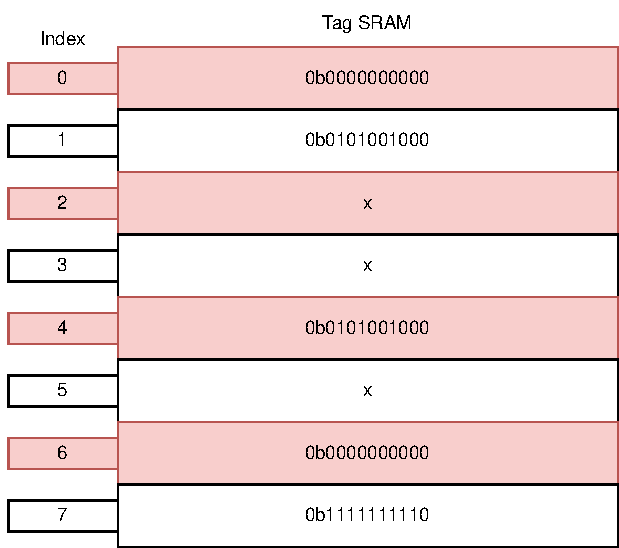
\includegraphics[width=0.7\textwidth]{tagsram.pdf}
 \centering
 \caption{Organizarea memoriei principale}
 \label{Figura:43}
 \end{figure}
 
 Se poate observa faptul că linile corespondente indecșilor 0 și 6 au același tag stocat, același lucru este sesizabil și în cazul indecșilor 1 și 4. În cazul identității a doi sau mai mulți indecsi, în memoria cache vor fi stocate blocuri care aparțin aceluiași tag, însă care cu un camp \textit{index} diferit.

Modul în care aceste două componente, cache SRAM și TAG SRAM comunică și stochează date, este arbitrat de o de-a treia entitate care poartă numele de  \textit{cache controller}. Pe lângă arbitrare, elementul de control are rolul de a interfata cu memoria, preluând date de la aceasta, conform adresei de acces cerute de procesor. De asemenea, răspunsul oferit înapoi procesorului este de o relevanță semnificativă.

 Elementul de control are 2 stări de răspuns posibile,  \textit{cache hit} și  \textit{cache miss}. Cache hit semnifică prezența datelor cerute pentru scriere sau citire de către procesor. Cache miss, pe de altă parte, indică lipsa acestor date din memoria cache.
 
 Stările cache hit și cache miss determină acțiuni diferite la nivelul controlerului în functie de tipul cererii procesorului, de citire sau de scriere.
 
La nivelul cache-ului predomină cererile de citire. Acestea sunt în general îndeplinite prin extragerea unui bloc din memorie, dacă acesta nu există, semnalându-se un cache miss. Daca blocul a fost deja pre-încărcat, se omite cererea de extragere din memoria principală, semnalându-se un cache hit, datele din adresa cerută fiind trimis de controler către procesor.

În cazul unei cereri de scriere în cache, lucrurile sunt puțin mai complexe. Există 2 mari strategi de îndeplinire a cereri de scriere, în cazul în care informațiile se găsesc deja în cache (cache hit), și anume \textit{write through} și \textit{write back}.

Write through implică actualizarea datelor atât la nivelul cache-ului cât și la nivelul memoriei principale, simultan.

Write back modifică datele doar la nivelul memoriei cache, urmând ca acestea să fie scrise în memoria principală odata cu înlocuirea blocului modificat. Semnalarea unui bloc modificat se va face printr-un bit suplimentar numic \textit{dirty bit}.

Dacă blocul în care se dorește scrierea nu se găsește în cache, controlerul va semnala un cache miss. Există din nou, 2 strategi relevante de a îndeplini cererea de scriere, acestea fiind \textit{write allocate} și \textit{no write allocate}.

Write allocate extrage blocul din memoria principală, dupa care modifică octeții relevanți ceruți de procesor.

No write allocate nu extrage blocul din memoria principală, acesta fiind tras în cache doar în momentul cererii de citire. Informațiile sunt prin urmare modificate doar la nivelul memoriei de date.


\newpage
\section{\centering IMPLEMENTARE}
\bigbreak
\subsection{ABSTRACȚIA MICROARHITECTURALĂ}
Microarhitectura reprezintă organizarea ierarhică și modulară a componentelor digitale prin care se realizează implementarea practică a unui microprocesor. Precum parcurgem acest nivel de abstracție, vor fi prezentate toate componentele de bază pe care un microprocesor le necesită pentru a funcționa la cel mai de bază nivel. Odată ce toate astfel de componente sunt definite, este posibilă organizarea lor conform arhitecturii RISC-V, rezultând astfel într-un procesor funcțional.

Componentele vor fi prezentate atât în format grafic, prin diagrame digitale, cât și prin codul aferent entității VHDL. Testarea entităților se va face printr-un \textit{testbench} VHDL, fiind prezentate formele de undă caracteristice.

 \subsection{SUMATORUL ȘI ARITMETICA NUMERELOR}
 Cea mai necesară operație pe care un sistem de calcul digital o poate executa este adunarea. Pe baza circuitului sumator se vor constitui alte componente digitale, precum \textit{program counter-ul}. Din cauza utilizării extensive a circuitelor sumatoare, acestea sunt adesea ținta unei multitudini de optimizări, rezultând astfel circuite de o complexitate digitală mai ridicată, dar cu o amprentă temporală redusă.
 
Sumatorul implementat în această lucrare este de tipul ripple adder, carry-ul propagându-se de la un full adder la altul. Avantajul acestei implementări este ușurința modelării hardware, dezavantajul fiind lipsa de optimizare temporală și spațială a operației.

Schema digitală a unui sumator full adder poate fi observată în Figura \ref{Figura:16}. Acesta are rolul de a executa suma a 2 biți, precum s-a prezentat la nivelul abstracției numerice.

 \begin{figure}[h!]
 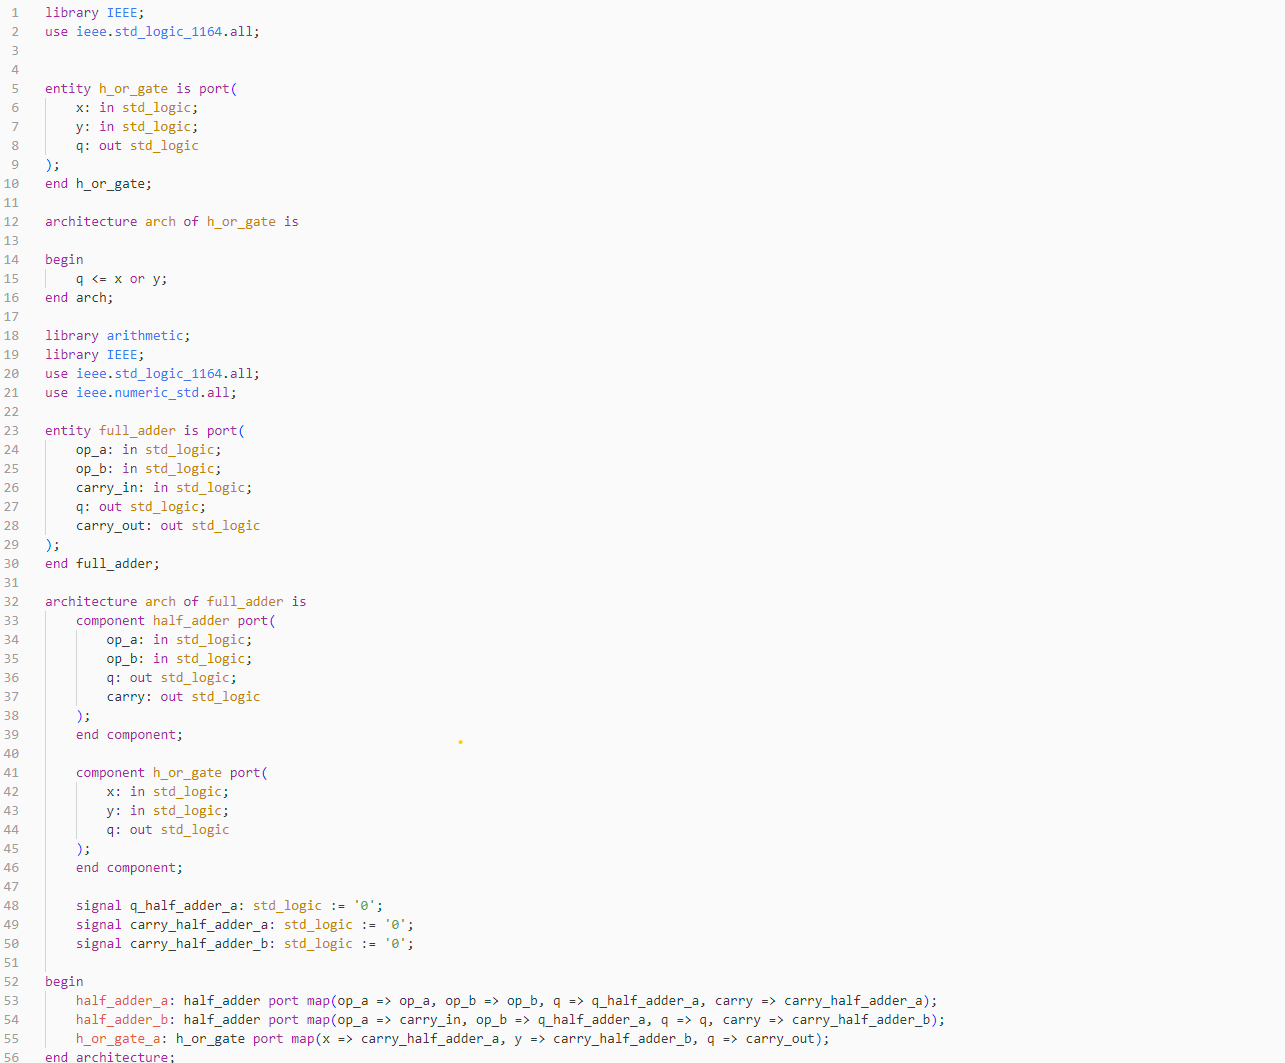
\includegraphics[width=1.03\textwidth]{fulladderVHDL.png}
 \centering
 \caption{Sumator integral și structura sa internă}
 \label{Figura:16}
 \end{figure}

Implementarea VHDL a entității cât și a arhitecturii sumatorului integral este redată prin secvența de cod aferentă Figurii \ref{Figura:25}. Se observă faptul că acestă entitate este construită prin relaționarea a două sumatoare pe jumătăți și a unei porți logice \textit{sau}.

 \begin{figure}[h!]
 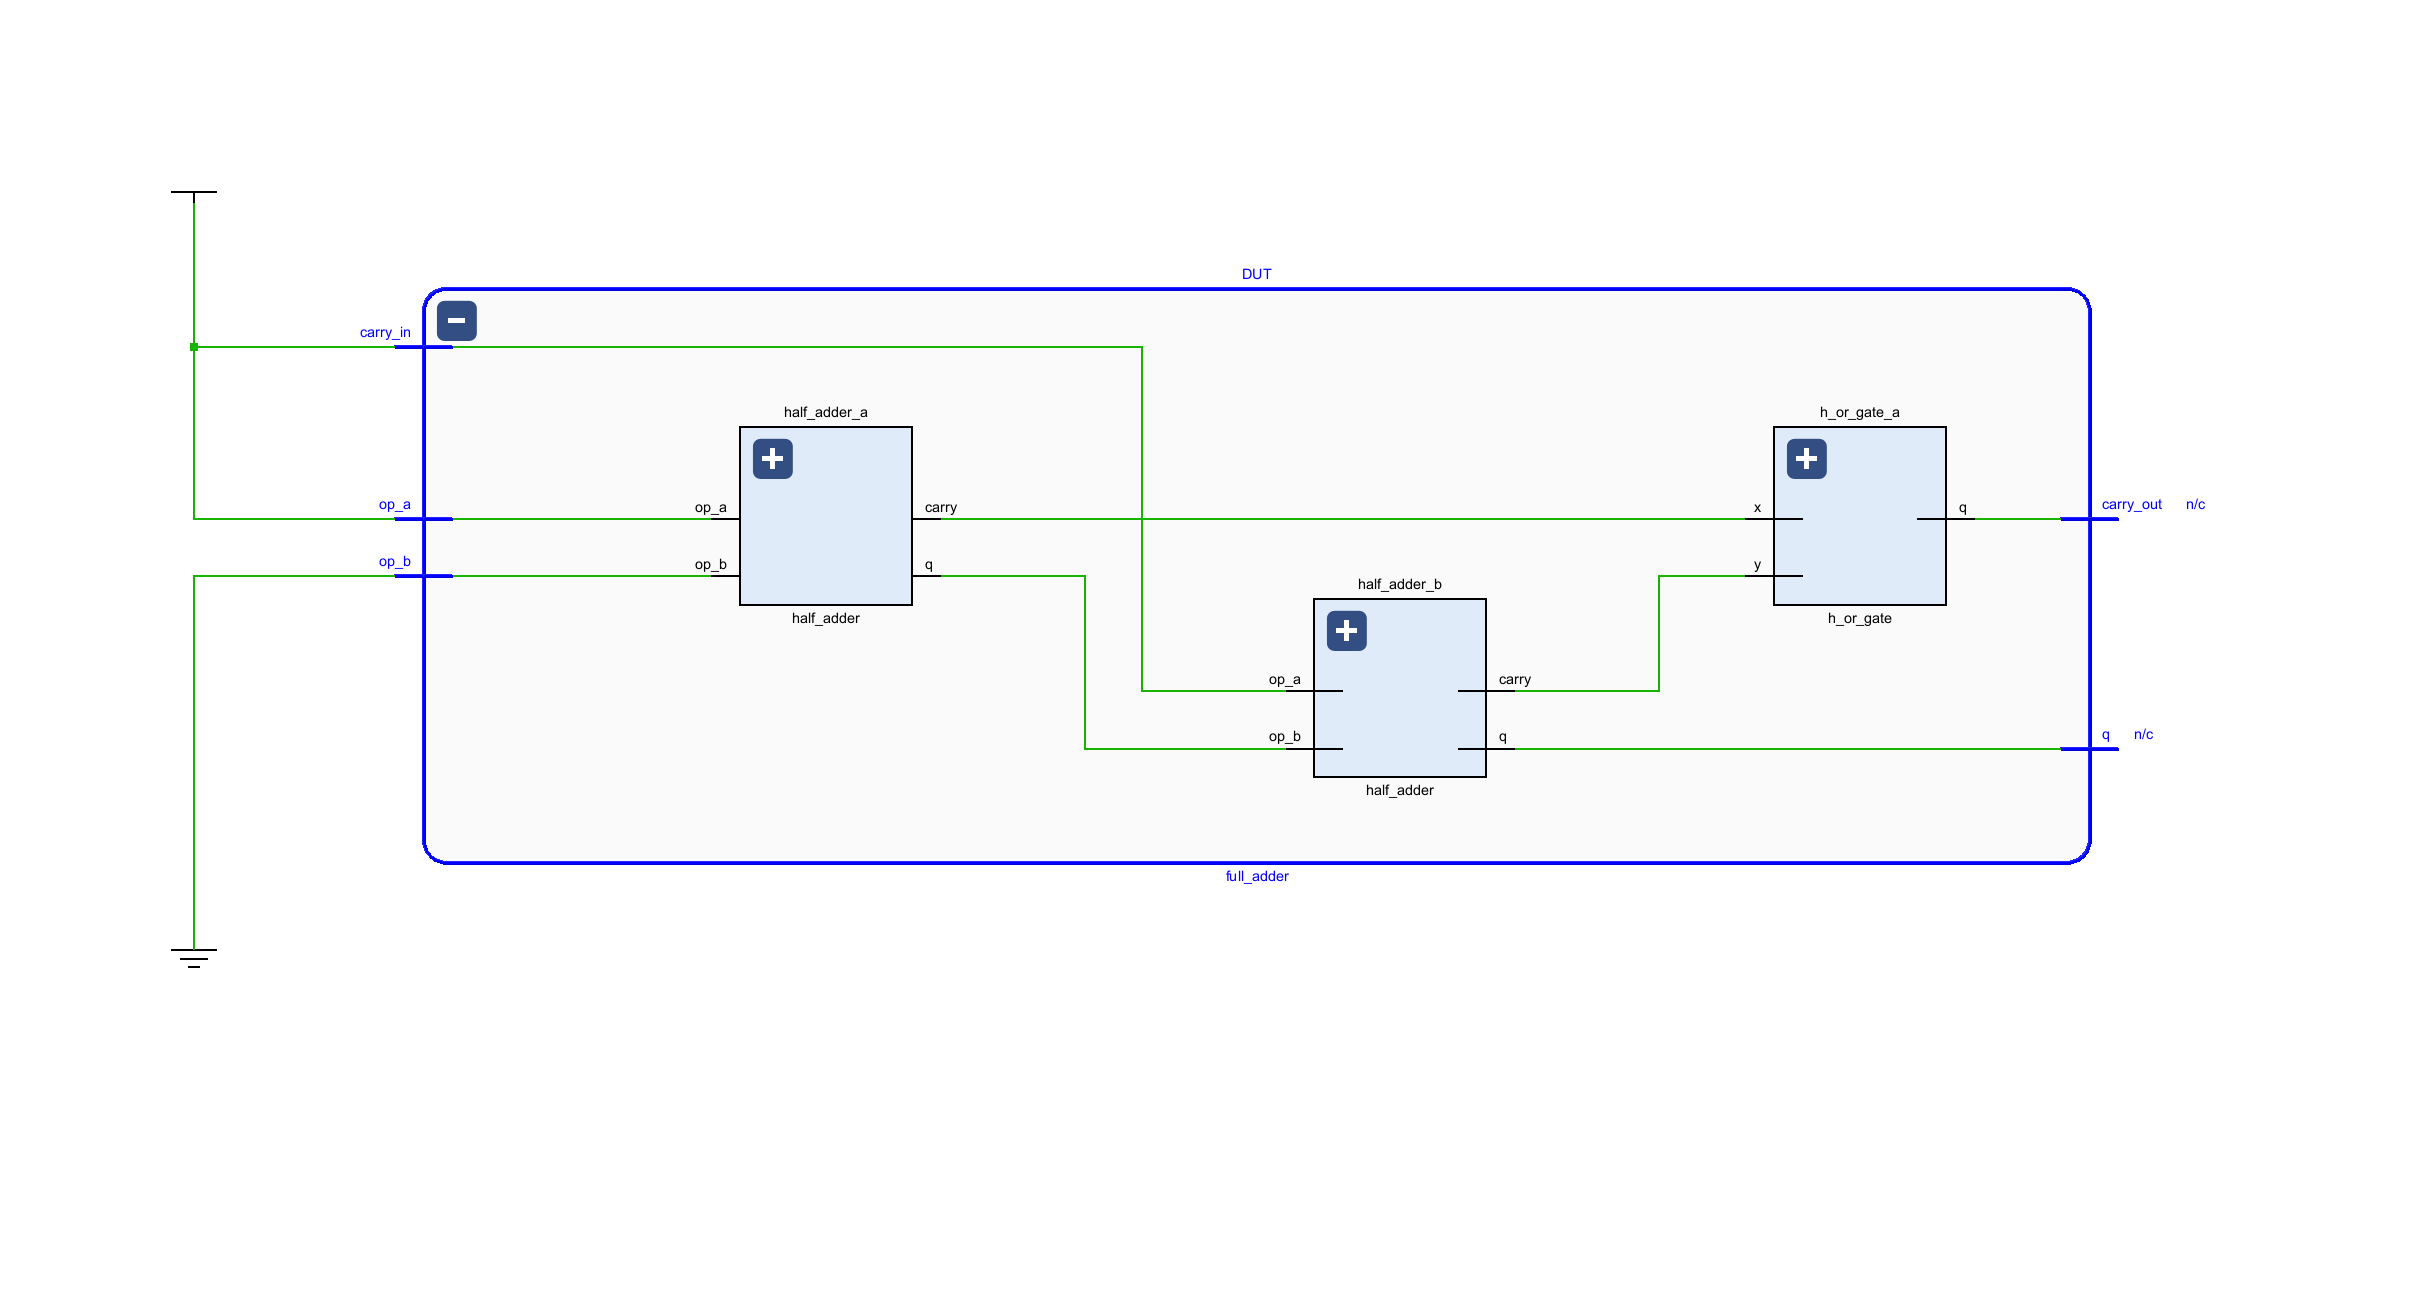
\includegraphics[width=0.9\textwidth]{fulladder.png}
 \centering
 \caption{Entitatea și arhitectura VHDL a sumatorului integral}
 \label{Figura:25}
 \end{figure}

Prin legarea serială a 8 sumatoare, rezultă entitatea fundamentală de adunare a procesorului nostru, și anume sumatorul de octeți sau \textit{byte adder}. Structura acestuia este prezentată în Figura \ref{Figura:17}. Se poate observa faptul ca cele 8 sumatoare sunt împărține în două grupuri de 4, fiecare numit \textit{nibble adder}.
 \begin{figure}[h!]
 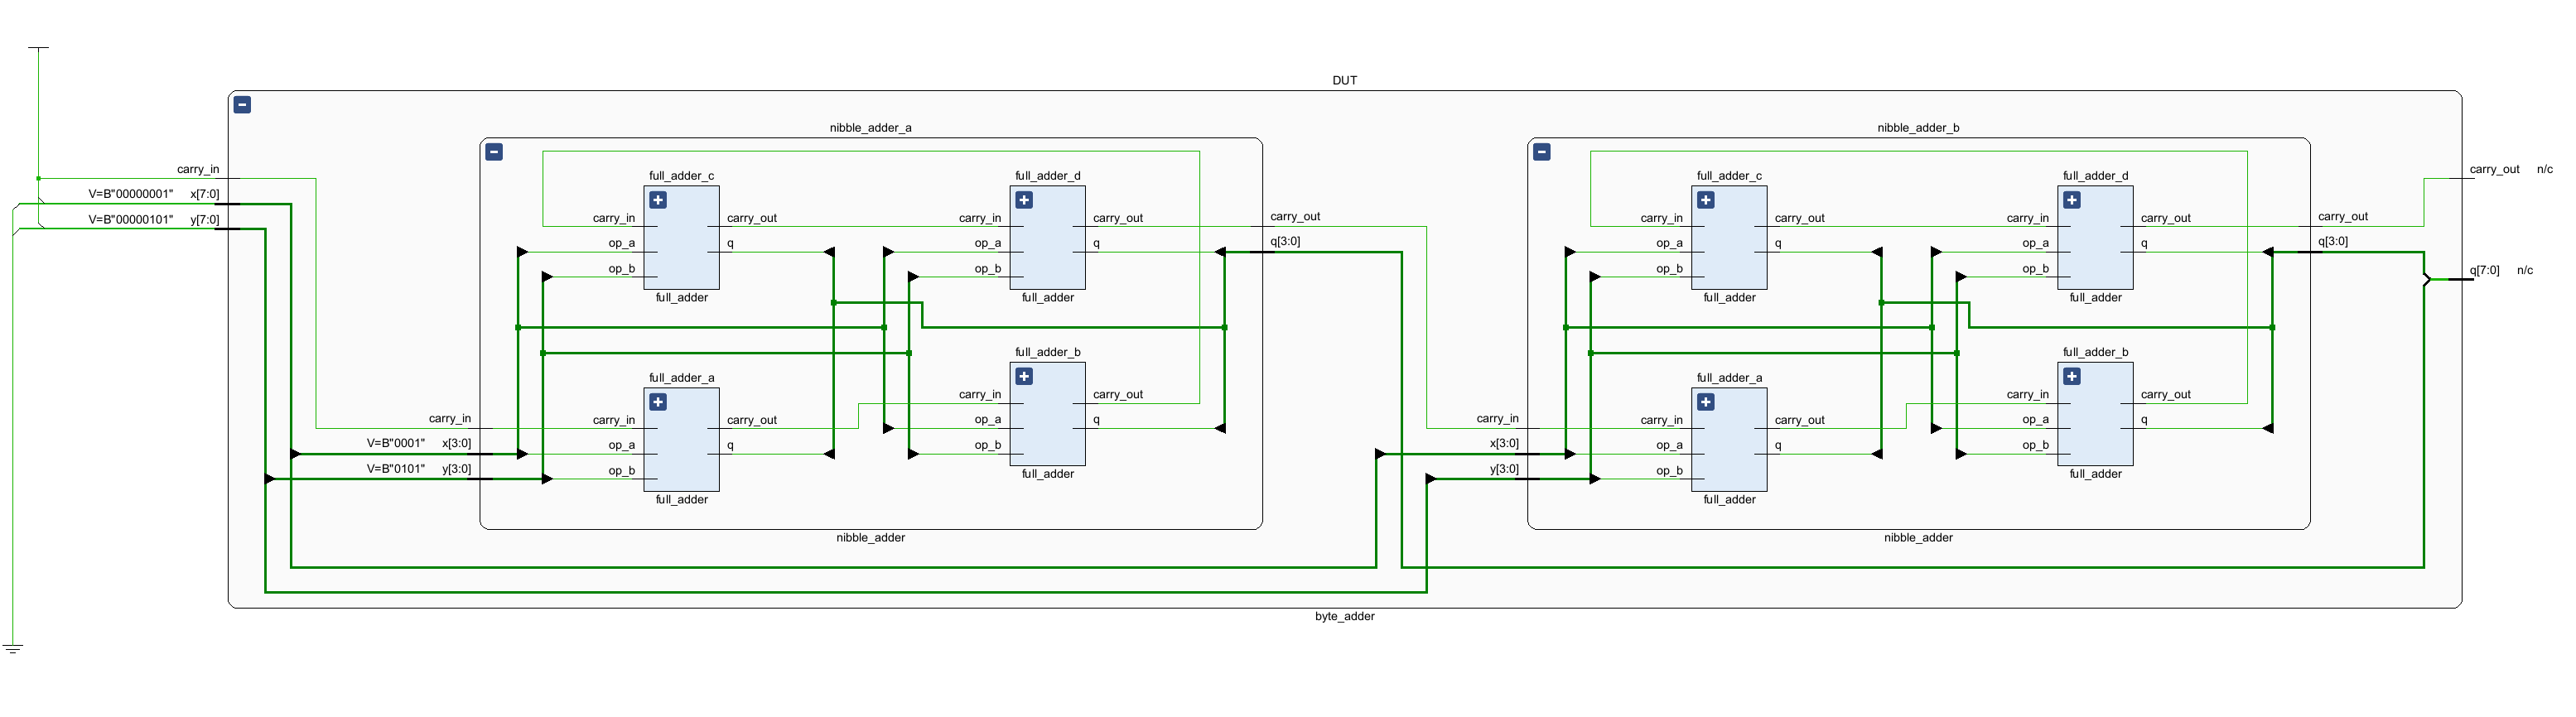
\includegraphics[width=0.9\textwidth]{byteadder.png}
 \centering
 \caption{Sumator de octeți si elementele constituente}
 \label{Figura:17}
 \end{figure}

Implementarea VHDL a structurii digitale prezentată mai sus se poate vedea în Figura \ref{Figura:26}.

 \begin{figure}[h!]
 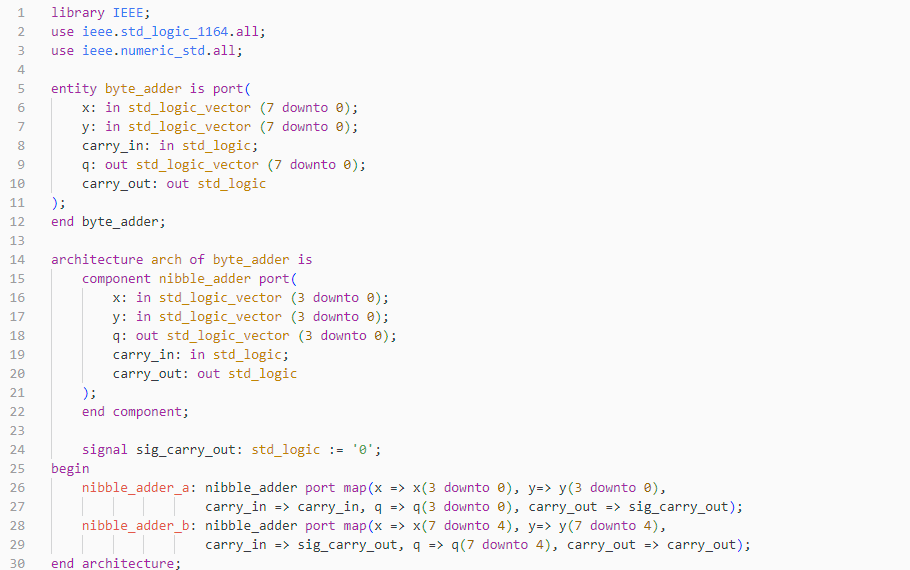
\includegraphics[width=1.0\textwidth]{byteadderVHDL.png}
 \centering
 \caption{Entitatea și arhitectura VHDL a sumatorului de octeți}
 \label{Figura:26}
 \end{figure}
 
Sumatorul de 32 de biți, cunoscut de asemenea ca sumatorul de cuvinte sau \textit{word adder} este prin urmare alcătuit din 4 sumatoare de octeți și poate fi văzut în Figura \ref{Figura:18}.

 \begin{figure}[h!]
 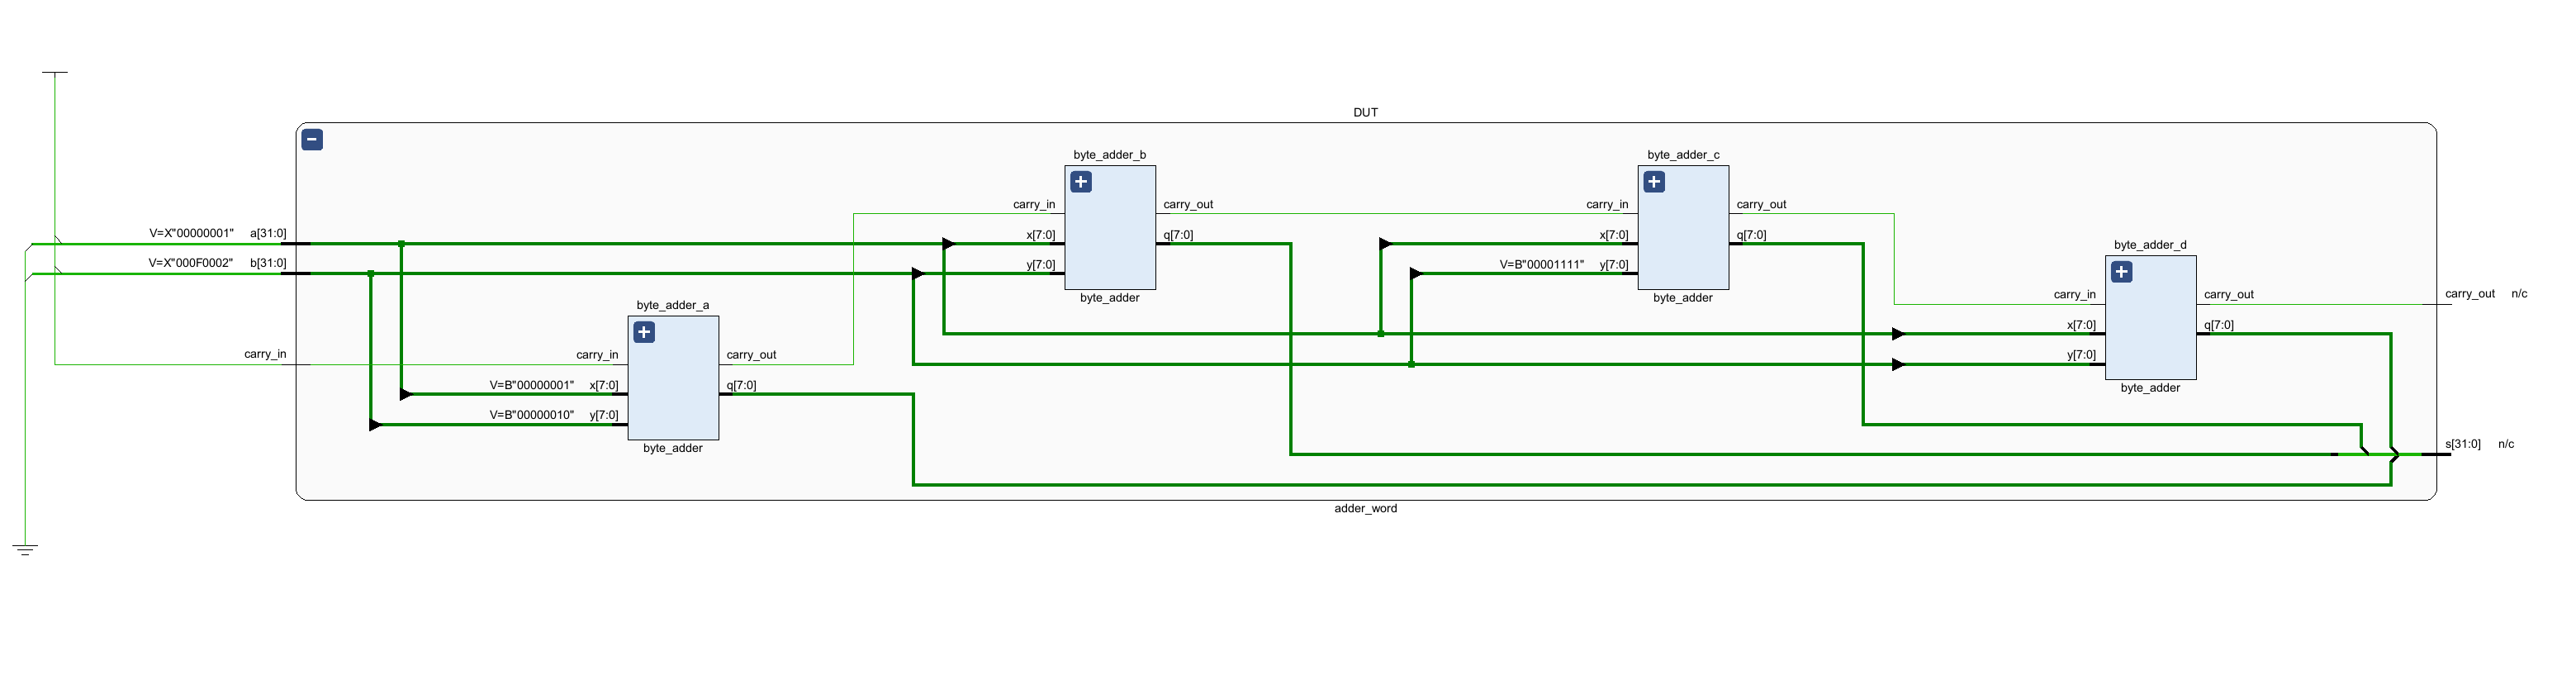
\includegraphics[width=0.9\textwidth]{32bitadder.png}
 \centering
 \caption{Sumator ripple carry adder de 32 de biți}
 \label{Figura:18}
 \end{figure}
 
Pentru a efectua operația de scădere, sunt necesare mai multe lucruri. În primul rând, avem nevoie de un inversor pentru a reprezenta forma complementară a numărului de scăzut. Pe lângă acest lucru, este necesar un multiplexor 2:1, a cărui rol este alegerea dintre numărul inversat și valoarea sa inițială, în funcție de operația dorită. Tabela \ref{Tabela:13} prezintă modul în care va funcționa o astfel de selecție.

\newpage
\begin{table}[h]
\centering
\caption{Efectuarea operaților în funcție de selecția multiplexorului}
\label{Tabela:13}
\begin{tabular}{ ||c|c|c|c|c|| }
 \hline
 A & B & Carry & Sel & Operație\\ 
 \hline  \hline
 0x0406001F & 0x031400A5 & 0 & 0 & Adunare \\
 \hline
 0x0013121F & 0x01144EB5 & 1 & 1 & Scădere \\
 
  \hline  
\end{tabular}
\end{table}

Se poate observa faptul că semnalul de \textit{carry} este setat pe 1 în cazul scăderii. Acest lucru formează practic complementul de 2 necesar scăderii, numarul fiind doar inversat în prealabil, rezultând un complement de 1.

Prin comasarea inversorului, a multiplexorului și a sumatorului rezultă astfel ceea ce vom denumi unitatea aritmetică. Schema digitală a acestuia se poate regăsi în Figura \ref{Figura:19}.

 \begin{figure}[h!]
 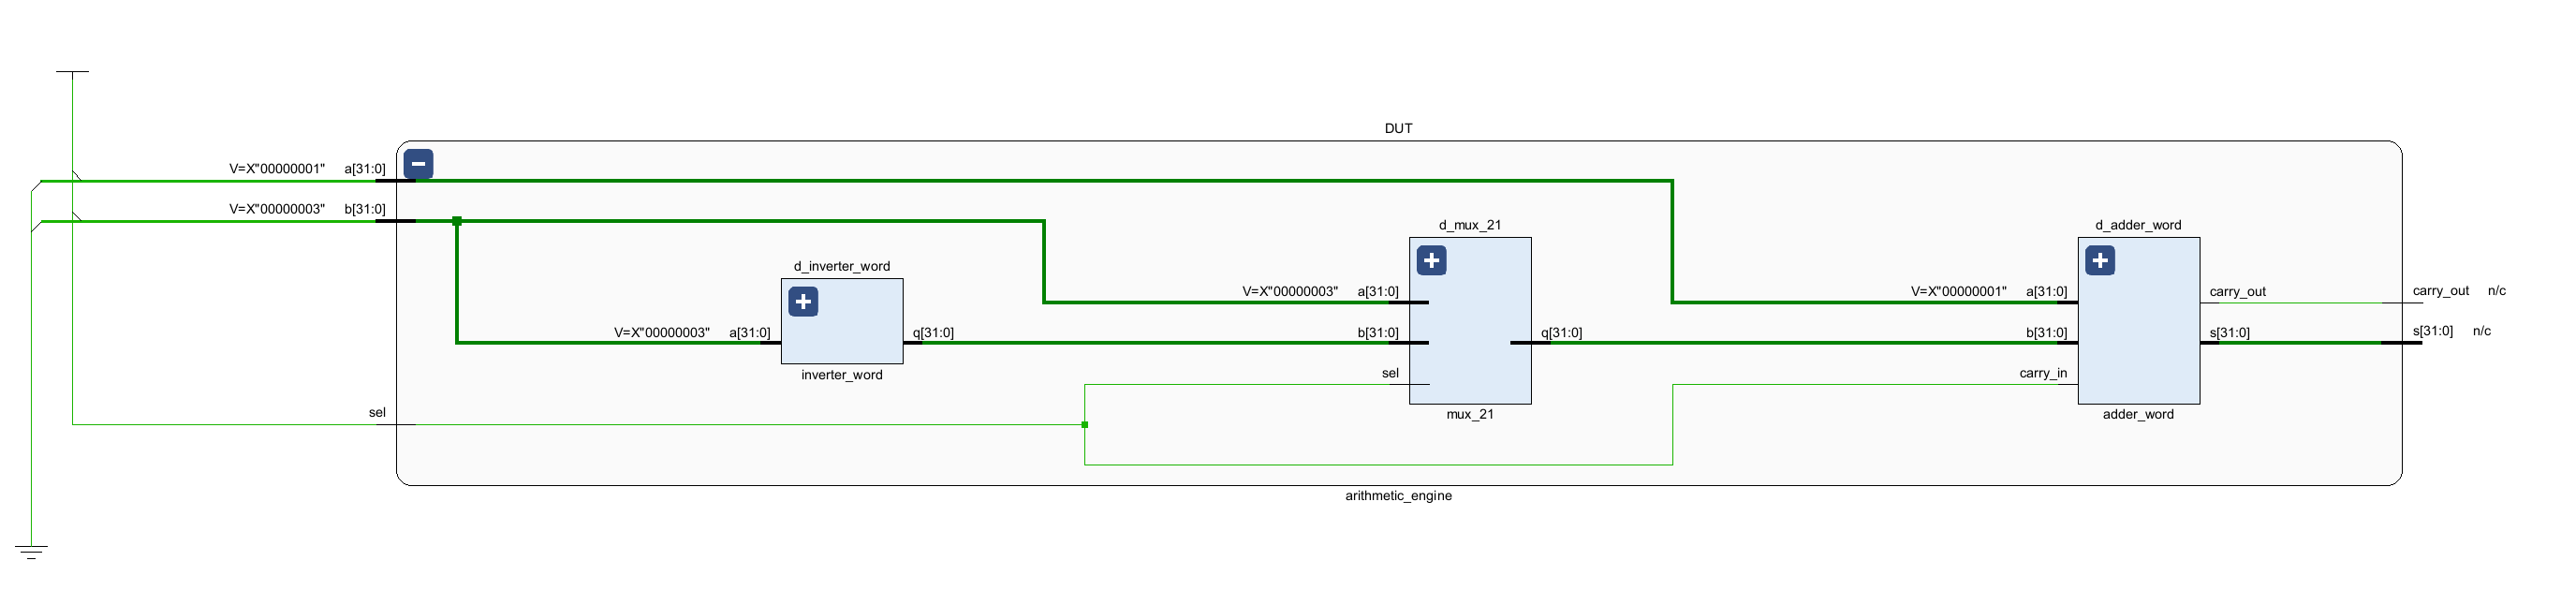
\includegraphics[width=0.9\textwidth]{ArithmeticEngine.png}
 \centering
 \caption{Unitatea aritmetică}
 \label{Figura:19}
 \end{figure}
 
Entitatea VHDL e unității aritmetice este redată prin codul prezentat în Figura \ref{Figura:60}.
 
 \begin{figure}[h!]
 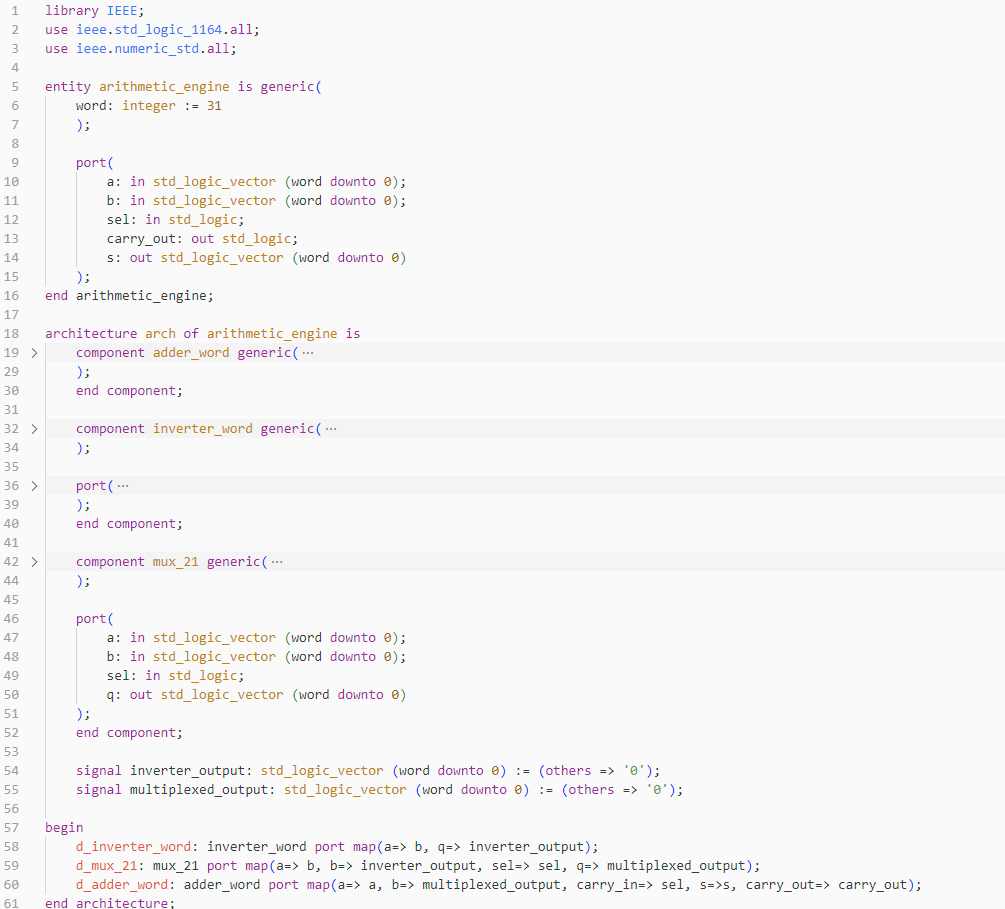
\includegraphics[width=0.75\textwidth]{arithmeticengineVHDL.png}
 \centering
 \caption{Entitatea și arhitectura VHDL a unității aritmetice}
 \label{Figura:60}
 \end{figure} 
 
 \subsection{OPERAȚII LOGICE ȘI UNITATEA LOGIC}
 
 Pe lângă operațile aritmetice, un procesor de asemenea are posibilitatea de executare a operaților logice pe biți. Microprocesorul nostru va avea implementarea hardware a funcțiilor SAU, ȘI, XOR. Toate entitățile necesare efectuării acestor operații vor fi comasate într-un element hardware denumit unitatea logică.
 
Figura \ref{Figura:20} conține schema digitală a motorului logic cât și a elementelor care-l definesc, cele 3 porți logice pe 32 de biți ȘI, SAU, XOR.
  \begin{figure}[h!]
 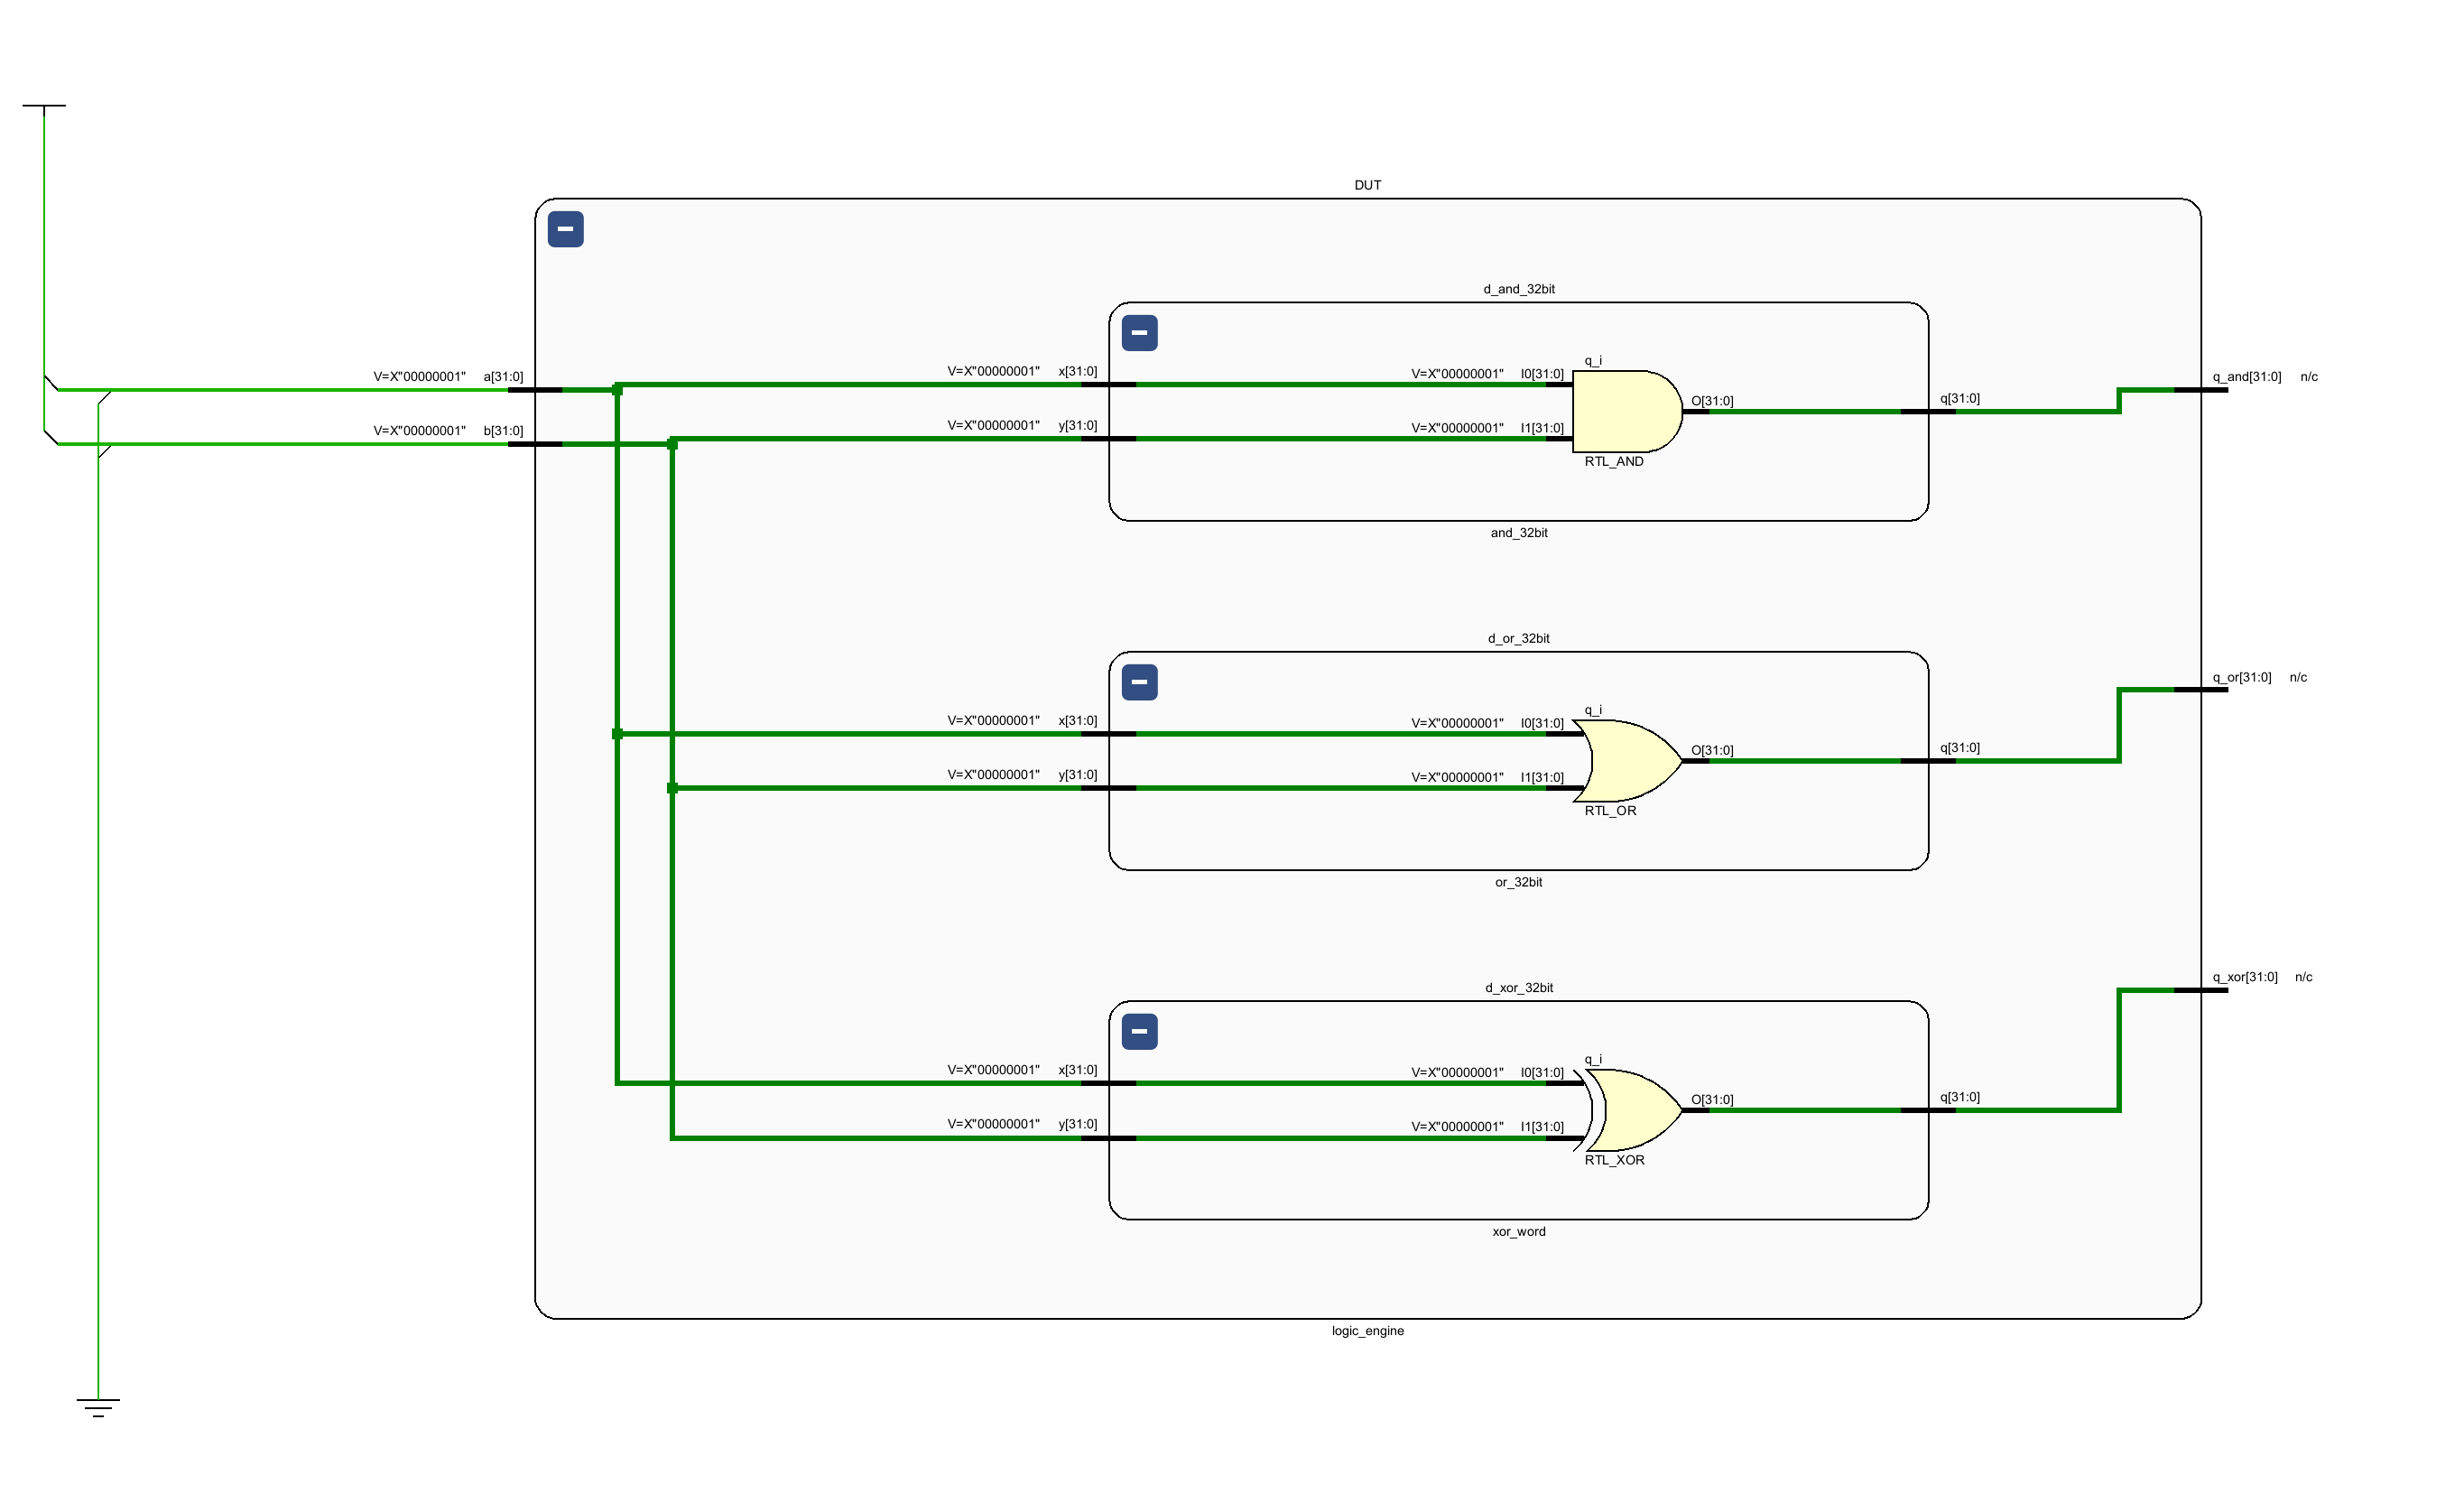
\includegraphics[width=0.81\textwidth]{LogicEngine.png}
 \centering
 \caption{Motorul logic și entitățile interne}
 \label{Figura:20}
 \end{figure}

Spre deosebire de calculul aritmetic, operațile logice sunt o trivialitate, lucru redat nu doar prin diagrama digitală, dar și prin codul asociat unității logice, prezent în Figura \ref{Figura:27}.

 \begin{figure}[h!]
 \includegraphics[width=0.62\textwidth]{logicengineVHDL.png}
 \centering
 \caption{Entitatea și arhitectura VHDL a unității logice}
 \label{Figura:27}
 \end{figure}
 
\newpage
\subsection{UNITATEA ARITMETICĂ ȘI LOGICĂ}

Unitatea aritmetică și logică este prima entitate ierarhică superioară pe care o vom reprezenta. Aceasta este formată din entitățile logice definite în prealabil, precum unitatea logică și cea aritmetică, dar conține de asemenea elementul pentru detecție de \textit{overflow}.

Utilitatea detectării unui posibil \textit{overflow} reiese în momentul în care dorim să executăm instrucțiunea \textit{less than}. În cazul a două numere, a și b, se va execut operația de scădere, semnul rezultant acestei operații determinând care dintre cele 2 numere este mai mare. O magnitudine negativă indică faptul ca primul număr, a, este mai mic, în schimb, semnul pozitiv indică spre b fiind numărul mai mic.

Precum se poate vedea în Tabela \ref{Tabela:14}, intervalul alocat numerelor pe 32 de biți este depăsit doar în cazul scăderii a douâ valori de semn opus.

\begin{table}[h]
\centering
\caption{Rezultatele posibile în cazul scâderii a 2 numere binare pe 32 de biți}
\label{Tabela:14}
\begin{tabular}{ ||c|c|c|c|| }
 \hline
 A & B & A-B & Overflow\\ 
 \hline  \hline
  $\ A \le 0$ & $\ B \le 0$ & $\ -2^{32} +1\le A-B \le 2^{31} - 1$ & Fără overflow \\
 \hline
  $\ A \ge 0$ & $\ B \ge 0$ & $\ -2^{32} +1\le A-B \le 2^{31} - 1$ & Fără overflow \\
 \hline
  $\ A \ge 0$ & $\ B \le 0$ & $\ 0 \le A-B \le 2^{32} - 2$ &  Overflow posibil\\
 \hline
  $\ A \le 0$ & $\ B \ge 0$ & $\ -2^{33} \le A-B \le 0$ &   Overflow posibil\\
 
  \hline  
\end{tabular}
\end{table}

De asemenea, semnul diferenței este mereu diferit de semnul descăzutului, în cazul unui overflow. Astfel, acesta poate fi detectat prin verificarea bit-ului de semn al diferenței în cazul în care operanzii sunt de magnitudini opuse. Tabela \ref{Tabela:15} prezintă cazurile în care se poate detecta overflow-ul, raportat la bit-ul de semn al operanzilor.

\begin{table}[h]
\centering
\caption{Valorile logice în cazul scăderii a 2 numere binare}
\label{Tabela:15}
\begin{tabular}{ ||c|c|c|c|| }
 \hline
 Bit de Semn A &  Bit de Semn B &  Bit de Semn A-B & Overflow\\ 
 \hline  \hline
  1 & 0& 1 & Fără overflow \\
  \hline
  1 & 0& 0 & Overflow \\
 \hline
  0 & 1& 0 & Fără overflow \\
 \hline
 0 &1& 1 &  Overflow \\
  \hline  
\end{tabular}
\end{table}

În Figura \ref{Figura:28} se poate vedea diagrama logică a circuitului de detecție al overflow-ului, acesta fiind construit conform ecuației logice deduse anterior.

 \begin{figure}[h!]
 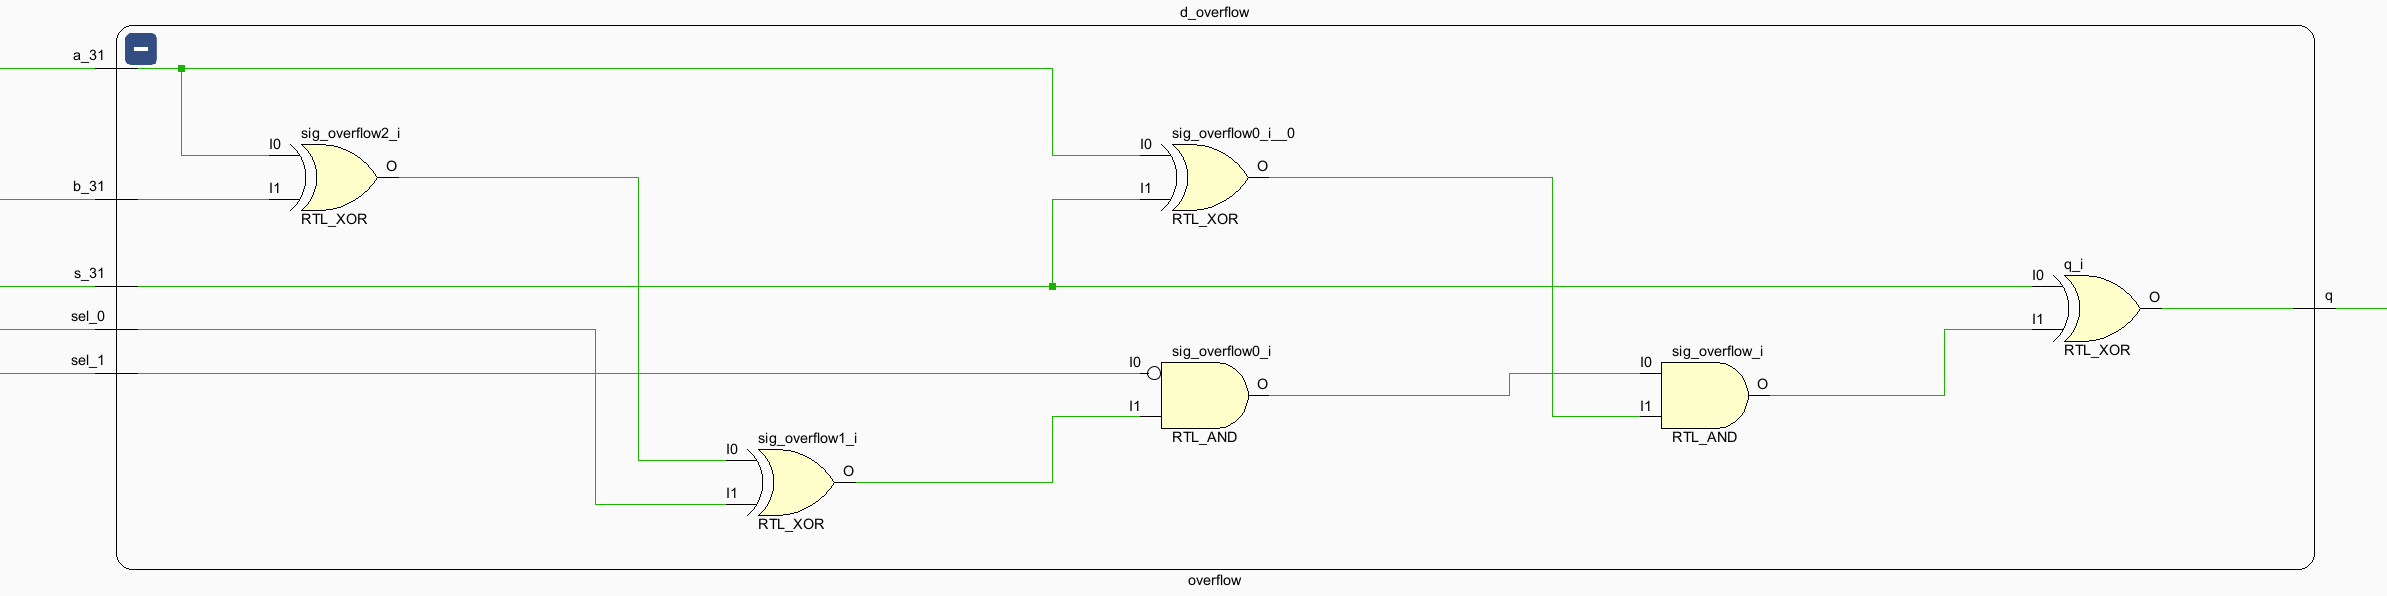
\includegraphics[width=0.7\textwidth]{overflow.png}
 \centering
 \caption{Diagrama logică a circuitului de detecție overflow}
 \label{Figura:28}
 \end{figure}
 
\newpage

Prin urmare, îmbinând toate elementele modelate anterior, rezultă schema digitală a unității aritmetice și logice, vizibilă în Figura \ref{Figura:21}. Figura \ref{Figura:29} prezintă codul entității și al arhitecturii VHDL aferent acestei componente.
\begin{figure}[h!]
 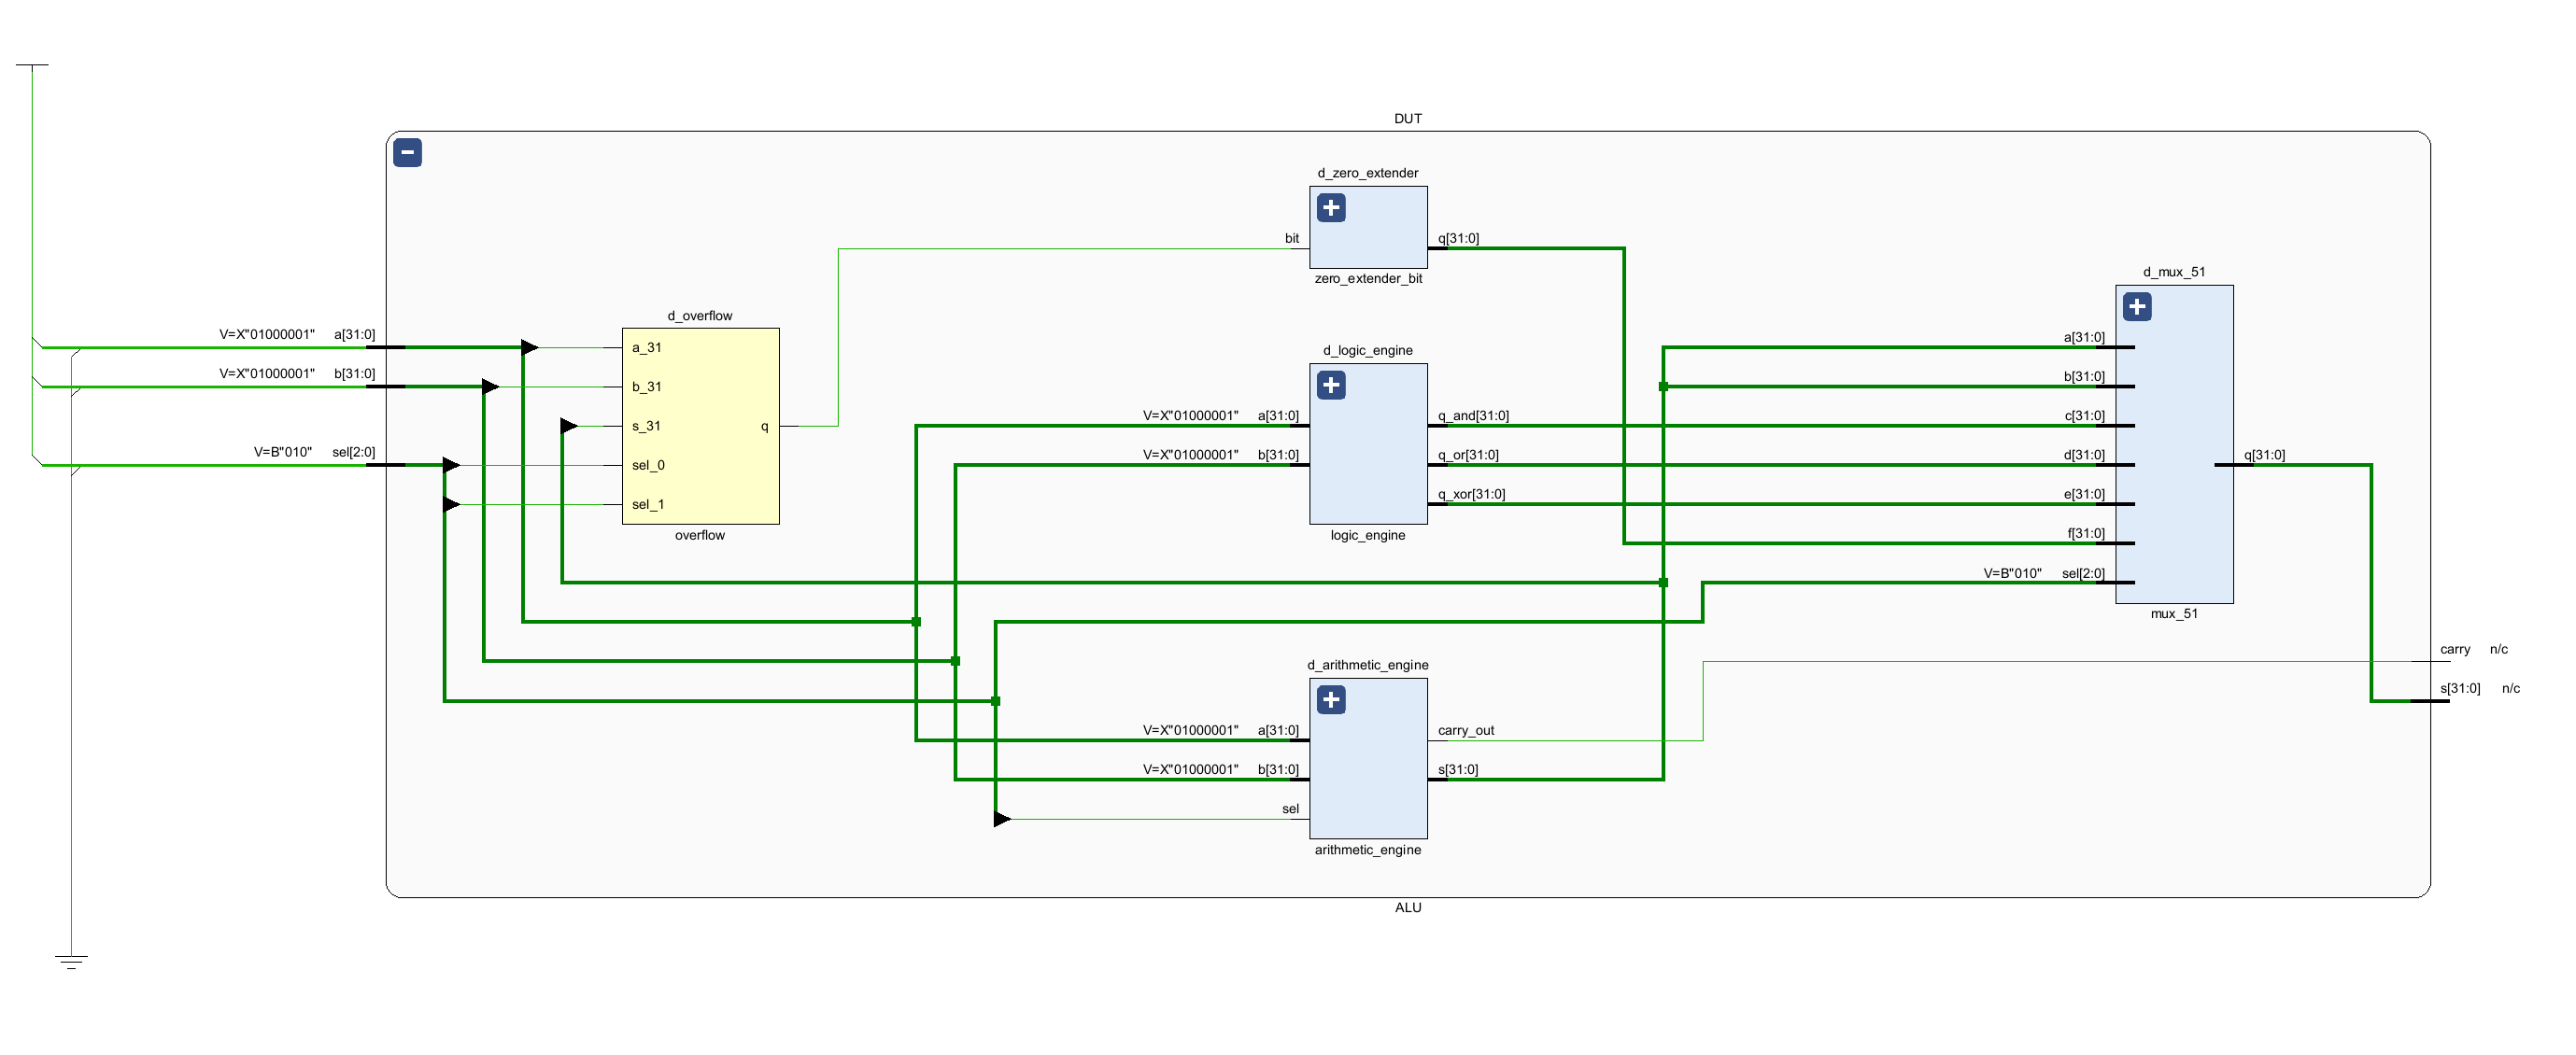
\includegraphics[width=0.9\textwidth]{ALU.png}
 \centering
 \caption{Unitatea aritmetică și logică}
 \label{Figura:21}
 \end{figure}


\begin{figure}[h!]
 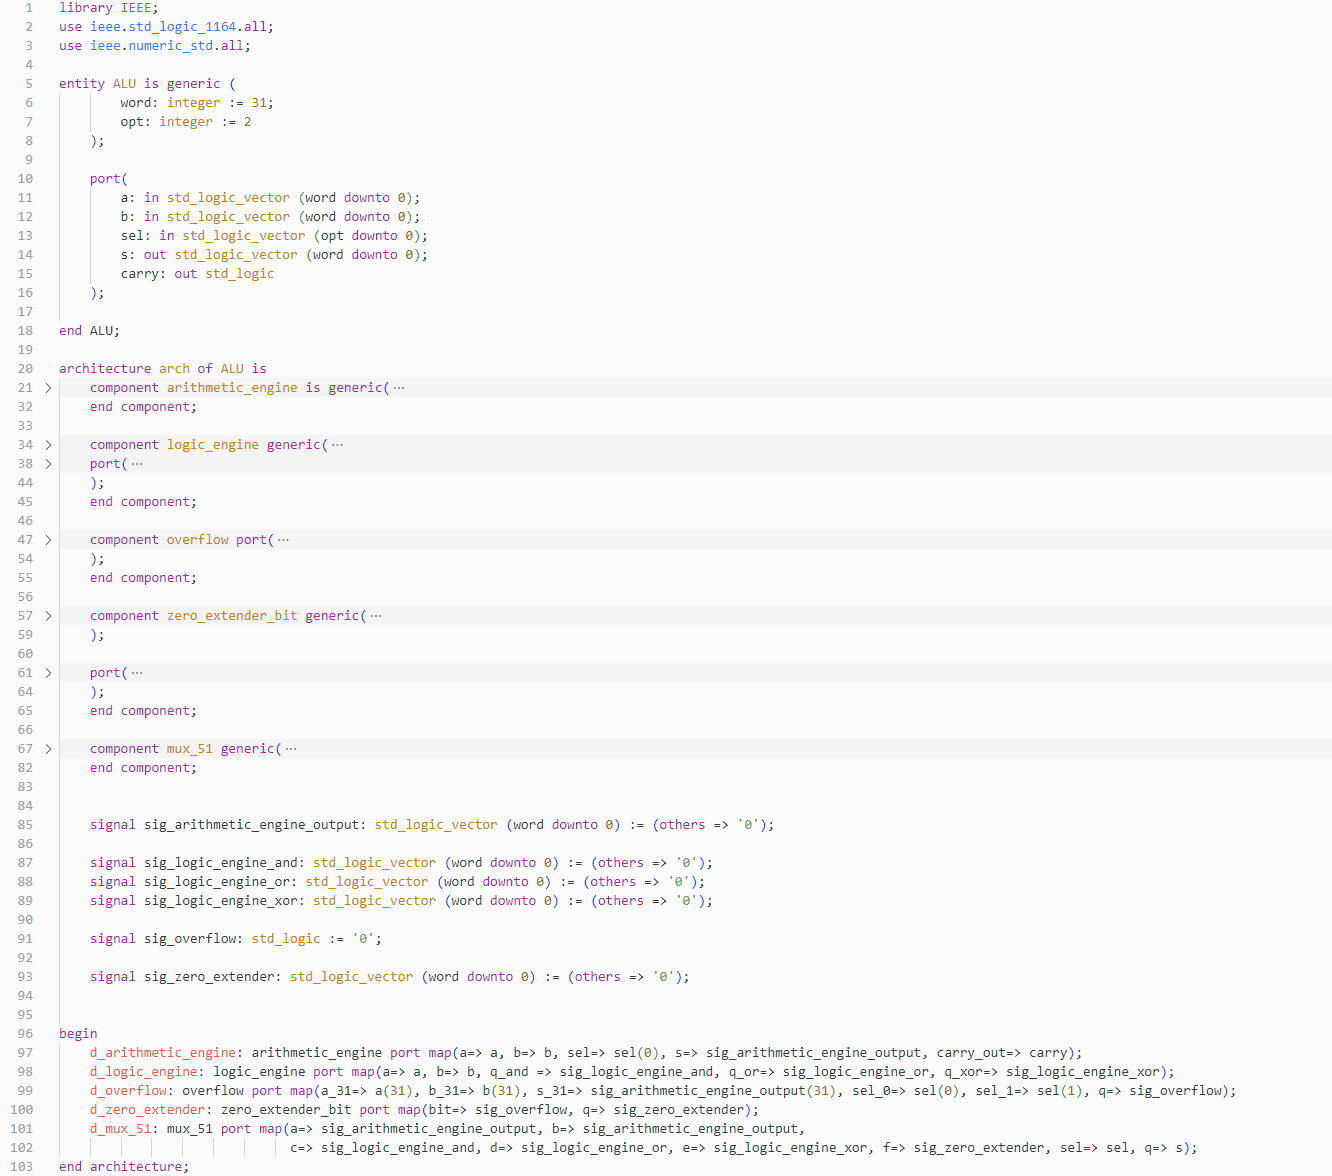
\includegraphics[width=0.9\textwidth]{aluVHDL.png}
 \centering
 \caption{Unitatea aritmetică și logică ca entitate VHDL}
 \label{Figura:29}
 \end{figure}
 
 \subsection{DISPOZITIVE DE MEMORARE}
 	Pentru a-și putea executa instrucțiunile într-un mod autonom, dar și pentru a putea stoca informații, procesorul va avea nevoie de dispozitive de memorare. Acestea dispozitive vin în mai multe forme, cel mai bine distingându-se memoriile volatile și nevolatile.
 	
 	 Diferența principală dintre aceste două memorii este faptul că memoria volatilă are nevoie de o constantă reactualizare a datelor, aceasta fiind construită pe baza unei matrici de capacitoare și tranzistoare. Prin urmare, pentru a simplifica design-ul hardware al procesorului, dar și pentru a reduce nivelul de abstracție, se vor utiliza memorii nevolatile.
 	 
 	 Memoria nevolatilă implementată în această lucrare se bazează pe celule de bistabile active pe front crescător. Datorită utilizării bistabilelor, latența de acces a datelor stocate în memorie este mică, principalul dezavantaj fiind implementarea practică, pricină costurilor ridicate ale unei astfel de memorii, utilizându-se mult mai multe tranzistoare decât în alternativa volatilă.
 	 
 	 Memoria din care se vor incărca instrucțiunile executate de procesor va purta numele de \textit{Memoria de instrucțiuni} iar, memoria generală distinată stocării datelor va purta numele de \textit{Memoria de date}.
 	 
	Accesul la nivelul ambelor memorii se va face la nivel de octet, fiecare cuvânt regasindu-se astfel la o adresă multiplu de 4. Pentru a acomoda încărcarea instrucțiuniilor din memorie, \textit{program counter-ul} va incrementa mereu la adresa instrucțiunii curente 4, obținându-se astfel adresa următoarei instrucțiuni de executat.
	
	Figura \ref{Figura:30} prezintă diagrama memoriei de instrucțiuni, așa cum aceasta este generată prin intermediul sintezei hardware oferite de Vivado.
	
\begin{figure}[h!]
 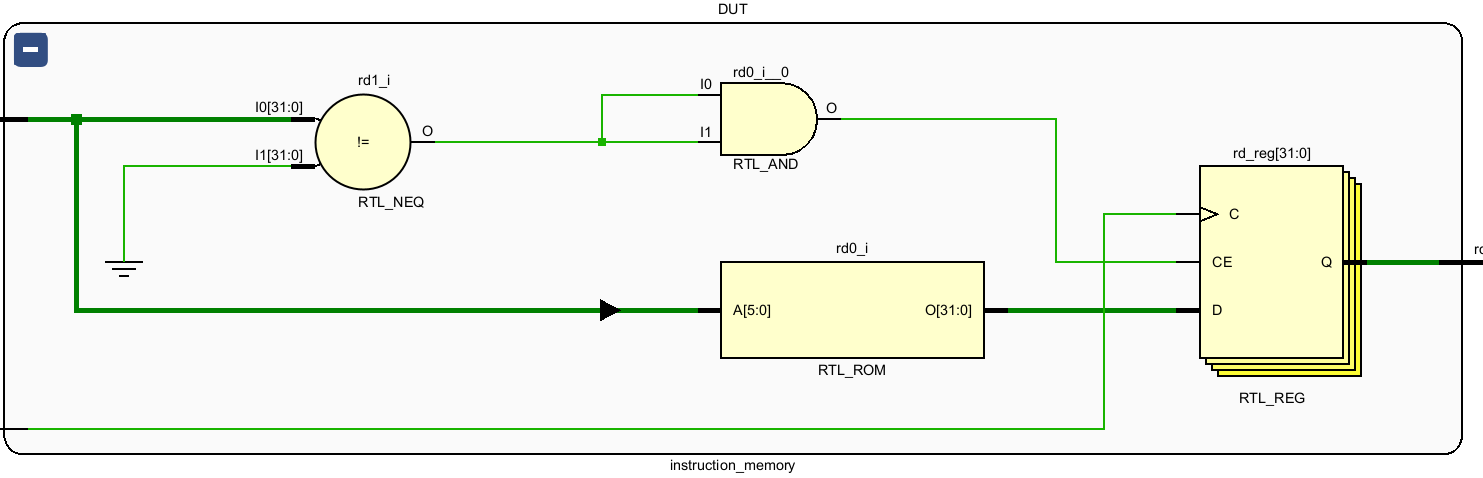
\includegraphics[width=0.95\textwidth]{instmem.png}
 \centering
 \caption{Memoria de instrucțiuni}
 \label{Figura:30}
 \end{figure}
 
 Codul entității VHDL al acestei memorii poate fi consultat în Figura \ref{Figura:31}. Este notabil modul în care ultimii 2 biți ai adresei instrucținii de executat sunt ignorați, cu ajutorul secvenței de cod \textit{address(7 downto 2)}.
 
\newpage
\begin{figure}[h!]
 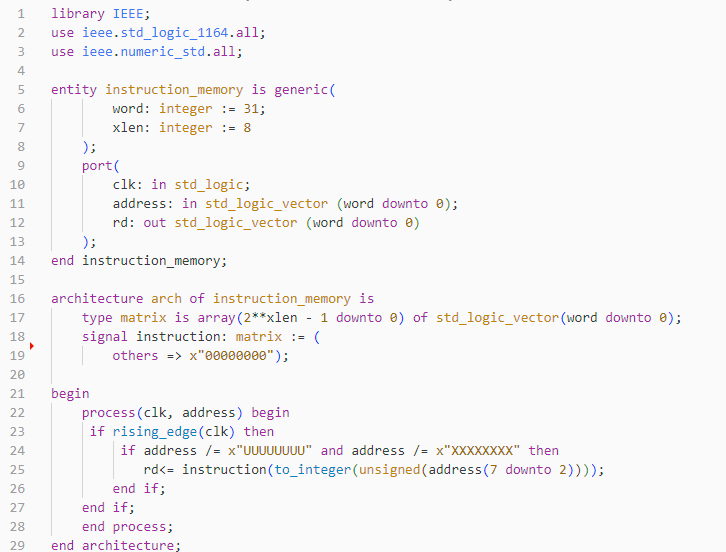
\includegraphics[width=0.9\textwidth]{instmemcode.png}
 \centering
 \caption{Memoria de Instrucțiuni ca entitate VHDL}
 \label{Figura:31}
 \end{figure}
 

În Figura \ref{Figura:32} putem observa design-ul hardware generat de sinteza automată pentru memoria de date. Se remarcă multiplexorul \textit{RTL} \textit{MUX}, rolul acestuia fiind de a lega la masă datele care ies din memorie, în cazul în care se dorește scrierea în aceasta, semnalul selector fiind reprezentat de \textit{write enable(we)}.
 
\begin{figure}[h!]
 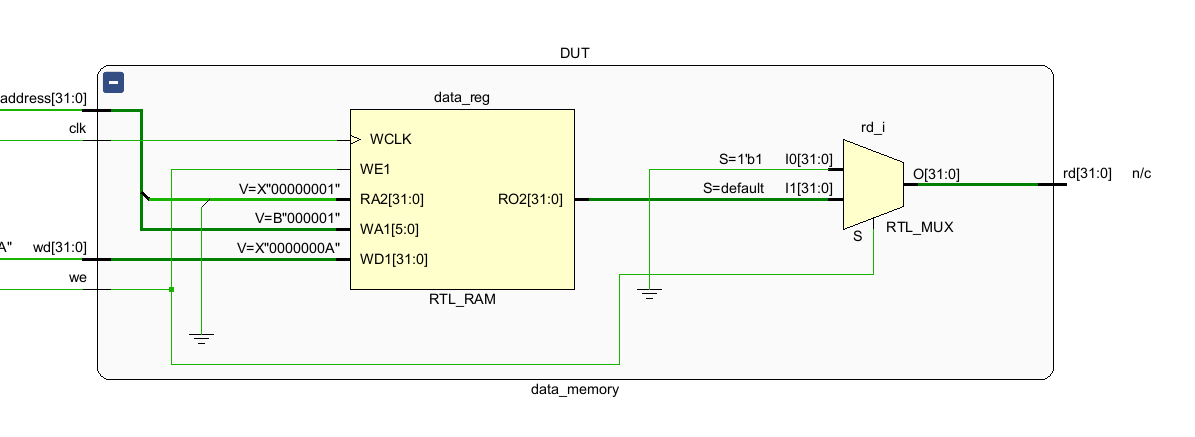
\includegraphics[width=0.9\textwidth]{datamem.png}
 \centering
 \caption{Memoria de Instrucțiuni ca entitate VHDL}
 \label{Figura:32}
 \end{figure}
  
 Codul entității VHDL al acestei memorii poate fi consultat în Figura \ref{Figura:33}. La fel ca în cazul memoriei de instrucțiuni, ultimii 2 biți ai adresei de intrare sunt ignorați, asigurând un comportament adresabil pe octeți.
 
 \begin{figure}[h!]
 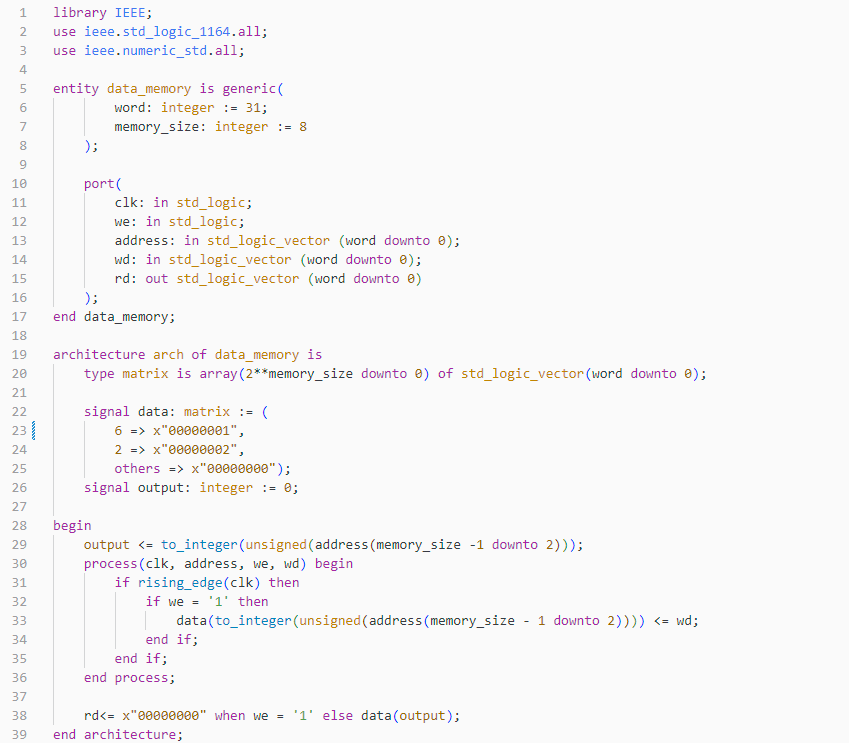
\includegraphics[width=0.9\textwidth]{datamemcode.png}
 \centering
 \caption{Memoria de Instrucțiuni ca entitate VHDL}
 \label{Figura:33}
 \end{figure}

 \subsection{FIȘIERUL DE REGISTRE}
 
 Precum s-a prezentata anterior, fișierul de registre al procesorului nostru acomodează 32 de registre cu funcții diverse, fiecare având o capacitate de stocare egală cu un cuvânt. Memorile implementate anterior sunt practic identice cu fișierul de registre, din punct de vedere al sintezeix automate,  datorită arhitecturii de tipologie nevolatilă.
 
 Pe lângă ciclul de tact și write enable, fișierul de registre are 4 intrări relevante,  \textit{rs1, rs2, rs3, wrs3} și 2 ieșiri \textit{rd1, rd2}. Rs1, rs2 și rs3 conțin adresele registrelor al căror acces îl dorim, wrs3 conținând cuvântul de scris în registrul indicat prin rs3. Implicit, rd1 și rd2 vor trimite în exterior cuvintele regăsite în registrele indicate de rs1 și rs2.
 
  Cea mai importantă caracteristică a acestui element de design este faptul că se poate realiza citirea datelor în parelel cu scrierea lor, astfel fiind posibilă executarea instrucțiunilor consecutive de efectuare a operaților cu datele din registre. Dintre toate cele 32 de adrese posibile, este intersiză scrierea datelor în registrul 0, acesta fiind legat la masă, facilitând efectuarea operaților cu 0, reducând astfel numărul de instrucțiuni necesare execuției unui program.
  

  \newpage  
  Figura \ref{Figura:34} conține diagrama generată de sinteza automată a fișierului de registre. Se observă modul de multiplexare a ieșirilor, acestea fiind mereu 0 în cazul accesului registrului 0.
 
  \begin{figure}[h!]
 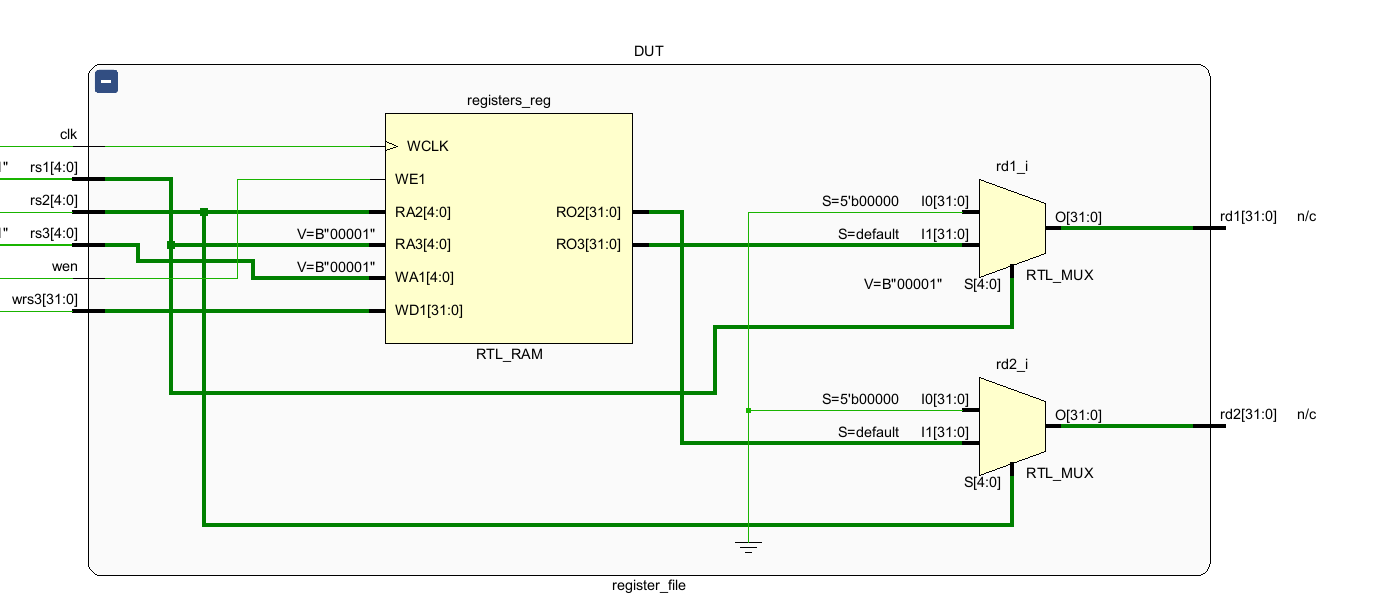
\includegraphics[width=0.95\textwidth]{regfile.png}
 \centering
 \caption{Fișierul de registre}
 \label{Figura:34}
 \end{figure}
 
Codul entității VHDL al acestui component se poate vedea în Figura \ref{Figura:35}.

  \begin{figure}[h!]
 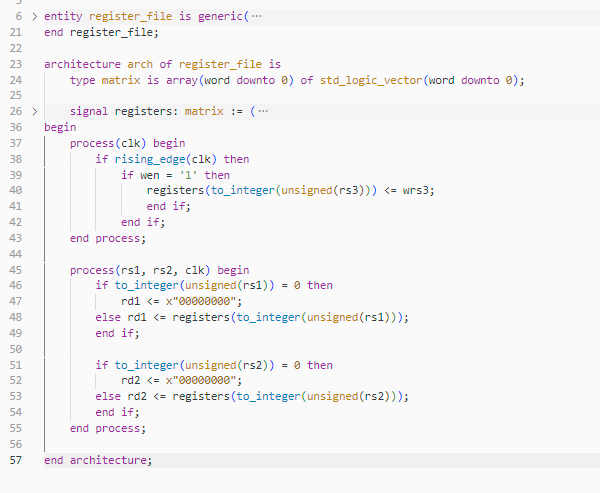
\includegraphics[width=0.9\textwidth]{regfilecode.png}
 \centering
 \caption{Fișierul de registre ca entitate VHDL}
 \label{Figura:35}
 \end{figure}
 
\subsection{EXECUȚIA SINCRONIZATĂ ȘI PROGRAM COUNTER-UL}

Pentru a executa sincron și secvențial instrucțiunile din memorie, avem nevoie de un modul care să realizeze incrementarea periodică a adresei instrucțiunii curente.

Entitatea destinată acestui scop poartă numele de \textit{program counter} și este formată dintr-un sumator, un modul generator de ciclu de tact și un bistabil pentru a transmite periodic indicele adresei de executat. Acestă implementare este suplimentată de un multiplexor 2:1, a cărui rol va fi selecția sursei instrucțiunii stocate în bistabil, în cazul în care se execută operația de  \textit{branch}.

Diagrama logică a acestui component poate fi observată în Figura \ref{Figura:36}.


 \begin{figure}[h!]
 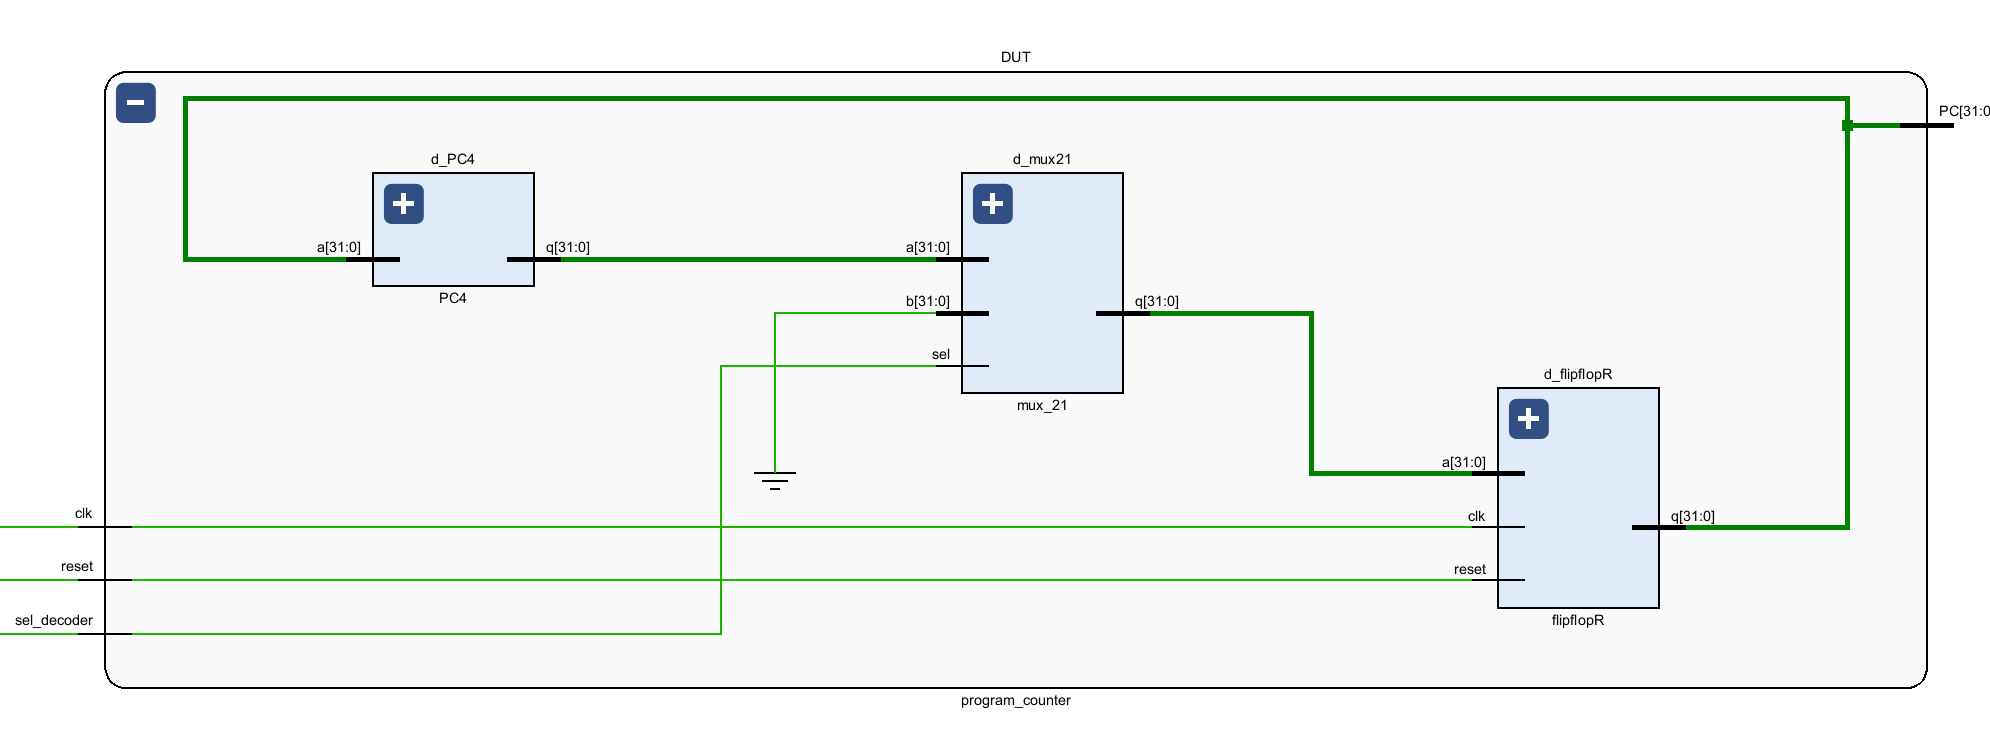
\includegraphics[width=0.9\textwidth]{programcounter.png}
 \centering
 \caption{Program counter-ul și elementele constituente}
 \label{Figura:36}
 \end{figure}
 
 Datorită abstractizării și modularizării implementării componentelor digitale definite până acum, program counter-ul nu necesită altceva decât definirea entității sale și a bistabilului constituent. Sumatorul și multiplexorul sunt definite în prealabil, fiind folosite de unitatea aritmetică și logică.
 
Figura  \ref{Figura:37} conține codul ce definește un bistabil sincron pe front crescător. Semnalul de reset are o importanță deosebită, initializând contorul și începând astfel execuția instrucțiunilor.
  \begin{figure}[h!]
 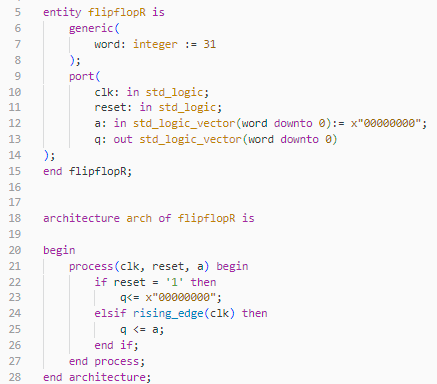
\includegraphics[width=0.41\textwidth]{bistabilcode.png}
 \centering
 \caption{Bistabilul sincron ca entitate VHDL}
 \label{Figura:37}
 \end{figure}

 \newpage
Codul aferent întregii entități VHDL a program counter-ului se regăsește în Figura \ref{Figura:38}.
 \begin{figure}[h!]
 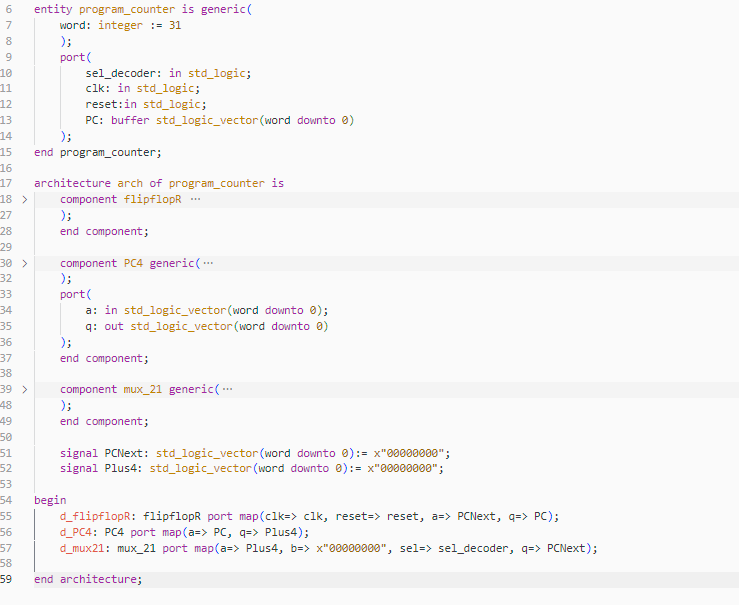
\includegraphics[width=0.815\textwidth]{programcountercode.png}
 \centering
 \caption{Program counter-ul ca entitate VHDL}
 \label{Figura:38}
 \end{figure}
 
 Program counter-ul nu are o utilitate de sine stătătoare, fiind nimic mai mult decât un sumator ciclic cu semnalul de tact. Acesta dobândește semnificație funcțională în momentul în care este legat la memoria de instrucțiuni, căreia ii va furniza indexul următoarei secvente de executat.
 
 Figura  \ref{Figura:39} prezintă o astfel de construcție logică, aceasta fiind practic entitatea de incărcare a instrucțiunilor în unitatea de control a procesorului.
 
  \begin{figure}[h!]
 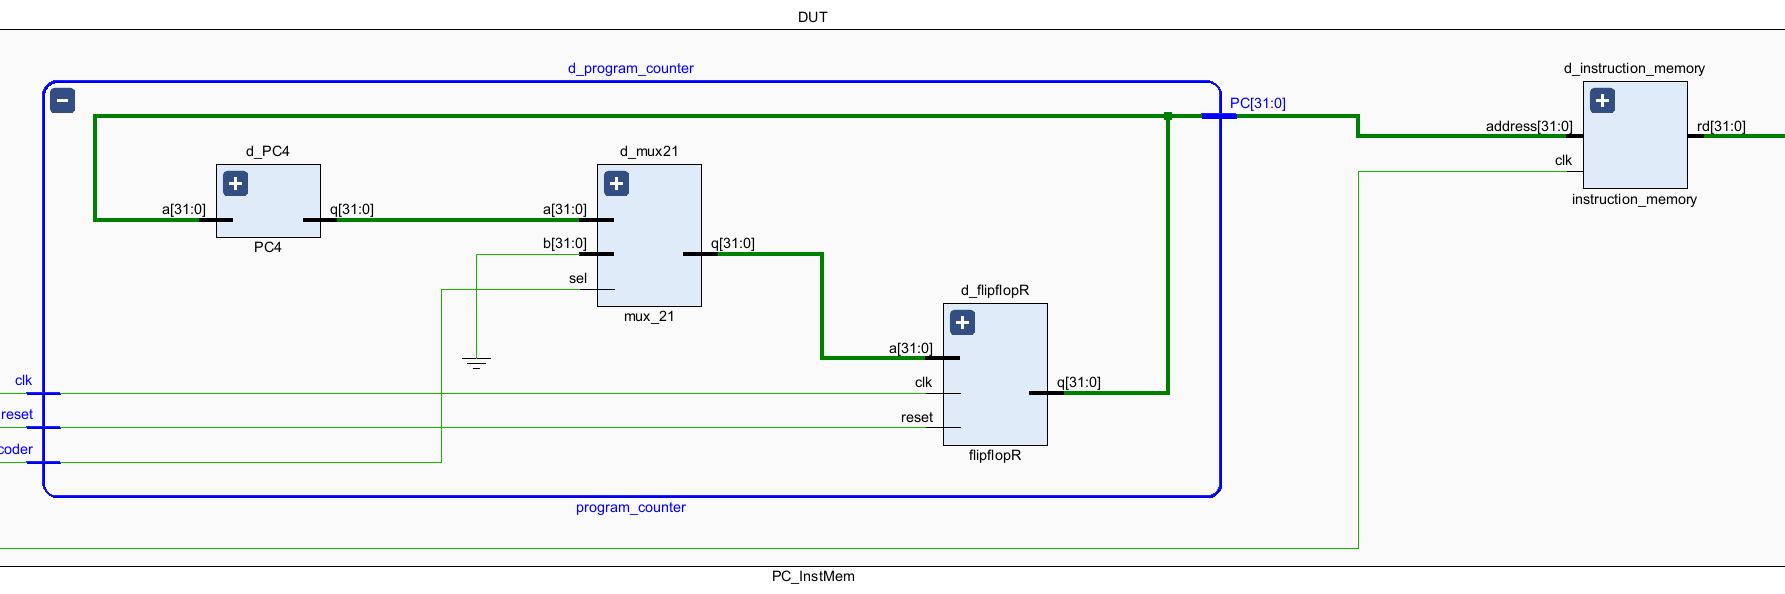
\includegraphics[width=1.0\textwidth]{pcinstmem2.png}
 \centering
 \caption{Construcția program counter - memoria instrucțiunilor}
 \label{Figura:39}
 \end{figure}
 
 Cum se poate observa, program counter-ul este practic un feedback loop a cărei execuție începe la acționarea semnalului de reset al procesorului, acesta oprindu-se, din punct de vedere funcțional, la întâlnirea instrucțiunii nule, instrucțiune care semnifică finalitatea programului de executat.
 
\subsection{DECODORUL DE INSTRUCȚIUNI}
 În lipsa unei entități care să interpreteze cuvântul de comandă transmis de memoria de instrucțiuni, procesorul nu are posibilitatea de a executa cod. Decodorul de instrucțiuni este elementul care va îndeplini un astfel de rol, trimițând biții de comanda mai departe elementelor digitale de execuție.
 
 Decodorul va fi modelat după instrucțiunile pe care procesorul le va implementa. Pentru a asigura o capabilitate computațională cât mai funcțională, păstrând gradul de complexitate în limite adecvate, se vor implementa decodificările unui subset de instrucțiuni din setul de bază aritmetic RISC-V. Subsetul implementat va asigura decodarea unei instrucțiuni din fiecare familie aparținând setului RISC-V, permițând astfel o eventuală extensie a hardware-ului pentru a suporta mai multe operații. Printe instrucțiunile implementate și decodate se numără următoarele:
 
 \begin{itemize}
\item Instrucțiunile aritmetice din familia R, asigurând calculul cu valorile din fisierul de registre. În acest set se vor regăsi comenzile \textit{add}, \textit{sub}, \textit{or}, \textit{and}.
\item Instrucțiunile din familia S, acestea asigurând încărcarea valorilor din registrul  \textit{rs2} în memoria de date la adresa calculată ca valoarea din  \textit{rs1} adunată la valoarea imediată furnizată. Comanda regăsită în acest set este \textit{sw (store word)}.
\item Instrucțiunile din familia I, acestea asigurând încărcarea valorilor îm registrul \textit{rs1} dintr-o adresă din memoria de date calculată ca suma unui offset furnizat ca valoare imediată și valoarea din registrul \textit{rs2}. Comanda \textit{lw(load word)} este instrucțiunea din acestă familie pe care decodorul o va implementa.
\item Instrucțiunile din familia B, acestea asigură posibilitatea execuției condiționate. Se testează egalitatea valorilor din registrele  \textit{rs1} și  \textit{rs2}. În caz de egalitate, program counter-ul sare la instrucțiunea egală cu adresa curentă adunată la valoarea imediate furnizată. Instrucțiunea de acest tip pe care o vom implementa este  \textit{beq}.
\end{itemize}

Din moment ce dorim o modularitate cât mai mare a hardware-ului, decodorul urmează să fie împărțit în două componente cu rol de decodificare. Primul component este practic decodorul principal, semnalând componentelor inferioare operațile care sunt pe cale de a fi executate. Decodorul secundar poartă numele de decodor aritmetic și are rolul de a orchestra modul de funcționare al unității aritmetice și logice. În mod practic, decodorul aritmetic va primi un cuvânt de comandă de la entitatea superioră, urmând ca  acel cuvant să fie interpretat, comenzile aritmetice fiind trimise unității de calcul.

Modul de funcționare al decodorului principal este prezentat în Tabela \ref{Tabela:16}. Câmpul \textit{Instr} reprezintă instrucțiunea pe care dorim să o executăm iar \textit{Op} reprezită codul operațional al acesteia.

 \begin{table}[h]
\centering
\caption{Decorodul principal}
\label{Tabela:16}
\begin{tabular}{ ||c|c|c|c|c|c|c|c|c|| }
 \hline
 Instr & Op & ALUOp & Reg Write & ImmSrc & ALUSrc & MemWrite & ResultSrc & Branch \\ 
 \hline
 \hline
 lw & 0000011 & 00 & 1 & 00 & 1 & 0 & 1 & 0 \\
 \hline
 \hline
  sw & 0100011 & 00 & 0 & 01 & 1 & 1 & - & 0 \\
 \hline
 \hline
  R & 0110011 & 10 & 1 & -- & 0 & 0 & 0 & 0 \\
 \hline
 \hline
  beq & 1100011 & 01 & 0 & 10 & 0 & 0 & - & 1 \\
 \hline
\end{tabular}
\end{table}

Câmpurile trimie de către decodor spre componentele inferioare au următoarele semnificatii:

\begin{itemize}
\item \textit{ALUOp} este cuvântul de comandă trimis decodorului aritmetic, acesta va indica în concordanță cu câmpul funct3 și funct7 operație pe care unitatea aritmetică și logică o va executa.
\item \textit{Reg Write} este bit-ul care indică fișerului de registre dacă se va realiza o scriere la nivelul său.
\item \textit{ImmSrc} va indica unității de extindere a semnului modul în care această operație trebuie realizată. Acest câmp reprezintă o necesitate din moment ce valorile imediate vin în mărimi diferite în funcție de tipul instrucțiunii executate.
\item \textit{ALUSrc} comută între semnalul primit de al doilea operand al unității aritmetice și logice. Dacă ALUSrc are valoarea 1, sursa celui de al doilea operand va fi furnizată de extensorul de semn, daca acest bit este resetat, sursa va proveni din fisierul de registre. 
\item \textit{Memwrite} înștiințează memoria principală ca urmează să se execute o scriere la nivelul său în momentul în care bit-ul este setat.
\item \textit{ResultSrc} are rolul de a comuta semnalele care vor fi stocate în fisierul de registre. Daca acest bit are valoarea 1, se va stoca în fișierul de registre cuvântul provenit din memoria principală. Valorea 0 indică stocarea în fișierul de registre al rezultatului furnizat de unitatea aritmetică și logică.

\item \textit{Branch} semnifică că urmează să se execute operație de branch, facându-se astfel un salt de la adresa actualei instrucțiuni la alta, rezultată din adunarea valori curente din program counter la o valoare imediată oferită de instrucțiune.
\end{itemize}

Codul aferent acestui decodor se poate consulta în Figura \ref{Figura:47}.

\newpage

 \begin{figure}[h!]
 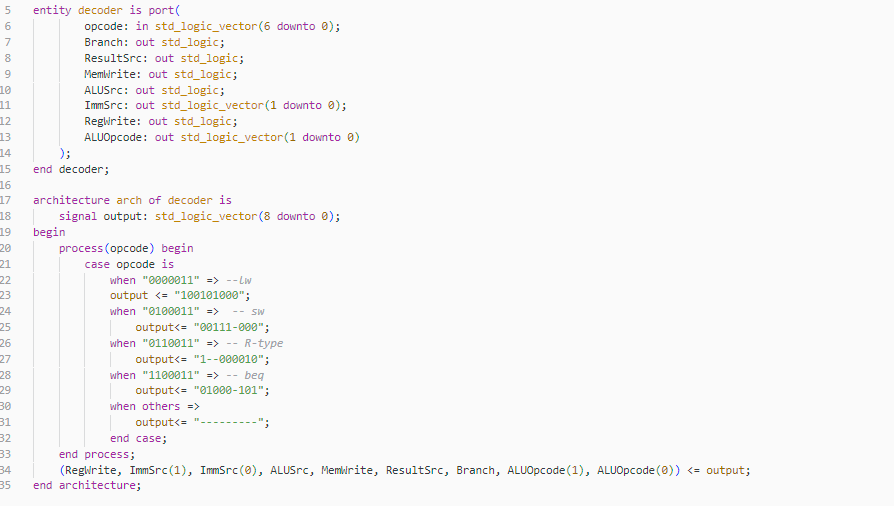
\includegraphics[width=0.94\textwidth]{decodercode.png}
 \centering
 \caption{Diagrama digitală a decodorului principal}
 \label{Figura:47}
 \end{figure}
 
 
 Sinteza automată înlocuiește logica combinațională cu memoria ROM, datele necesare fiind stocate la adresele acestei memorii. În funcție de cuvântul instrucțiunii, multiplexorul intern al acestei memorii comută semnalul de ieșire, trimitând astfel componentelor subordonate semnalele de control corecte. Figura \ref{Figura:45} prezintă acest fapt.
 
  \begin{figure}[h!]
 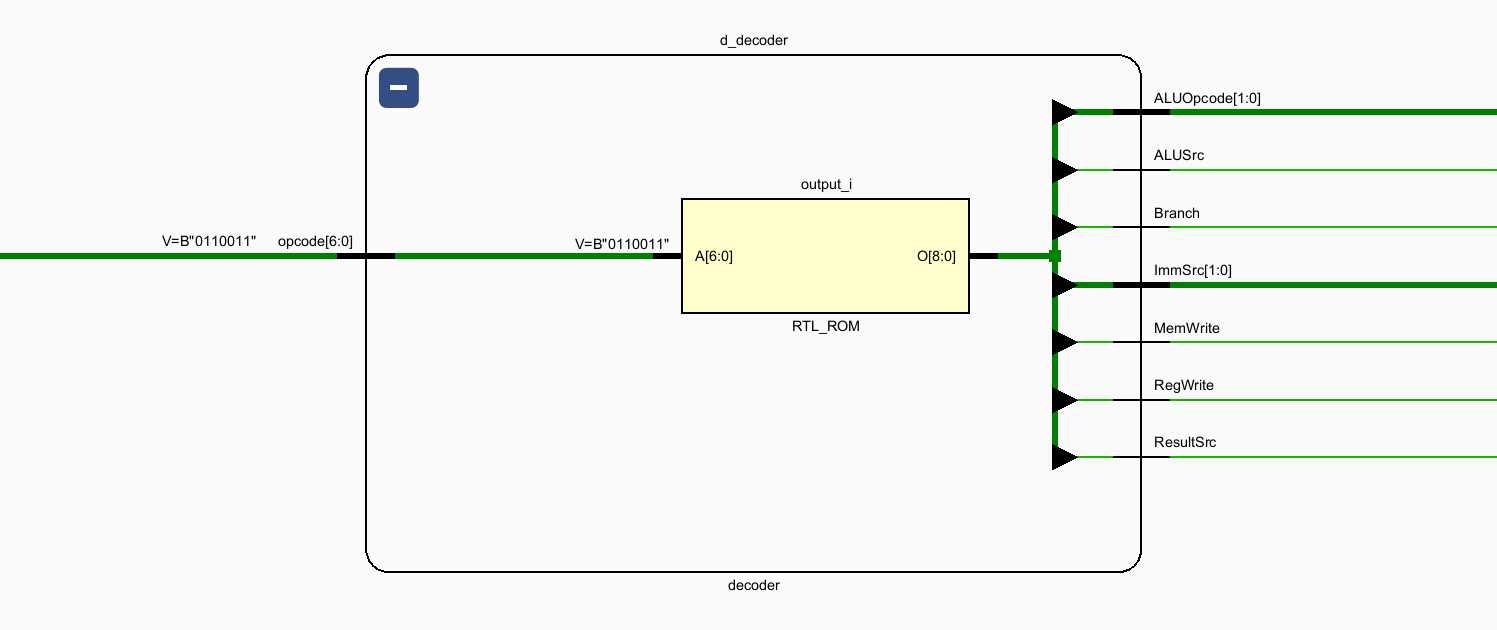
\includegraphics[width=0.94\textwidth]{decoder.png}
 \centering
 \caption{Entitatea VHDL a decodorului principal}
 \label{Figura:45}
 \end{figure}

Decodorul aritmetic pe de altă parte, are rolul de a semnala unității de execuție ce tip de operație este cerută de instrucțiune. Tabela \ref{Tabela:17} prezintă modul său de funcționare. ALUControl este semnalul de ieșire al acestei componente spre unitatea aritmetică și logică, specificând multiplexorului acesteia operația cerută.

\newpage
 \begin{table}[h]
\centering
\caption{Decorodul aritmetic}
\label{Tabela:17}
\begin{tabular}{ ||c|c|c|c|c|| }
 \hline
 ALUOp & funct3 & {op(5), funct7} & ALUControl & Instrucțiune\\ 
 \hline
 00 & --- & -- & 000(scădere) & lw, sw\\
 \hline
 01 & --- & -- & 001(adunare) & beq\\
 \hline
 10 & 000 & 00, 01, 10 & 000(adunare) & add\\
 \hline
 10 & 000 & 11 & 001(scădere) & sub\\
 \hline
 10 & 010 & -- & 101(mai mic decât) & slt\\
 \hline
 10 & 110 & -- & 011(sau) & or\\ 
\hline
 10 & 111 & -- & 010(și) & and\\
 \hline
\end{tabular}
\end{table}

Pe lângă datele provenite de la unitatea superioară, decodorul aritmetic extrage din cuvântul instrucțiunii datele \textit{funct3, op din bitul al 5-lea, funct7}, acestea având rol în specificarea detaliată a operației. Combinația op(5), funct7 selectează între adunare în cazul instrucțiunilor aritmetice R, funct3 fiind, tot pentru această familie de instrucțiuni, selectorul operaților logice.

Codul VHDL al decodorului aritmetic este prezentat în Figura  \ref{Figura:46}.

  \begin{figure}[h!]
 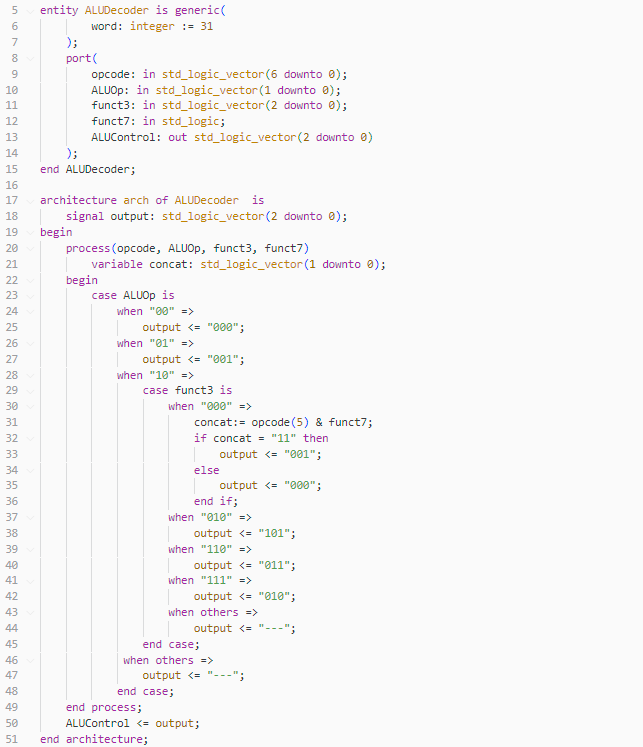
\includegraphics[width=0.75\textwidth]{aludecodercode.png}
 \centering
 \caption{Entitatea VHDL a decodorului aritmetic}
 \label{Figura:46}
 \end{figure}

\newpage

Entitatea logică generată de sinteza VHDL pentru decodorul aritmetic se poate vedea în Figura \ref{Figura:47}. Acesta este practic format prin legarea în cascadă a 3 multiplexoare, fiecare comutând după un semnal de intrare diferit.
 
  \begin{figure}[h!]
 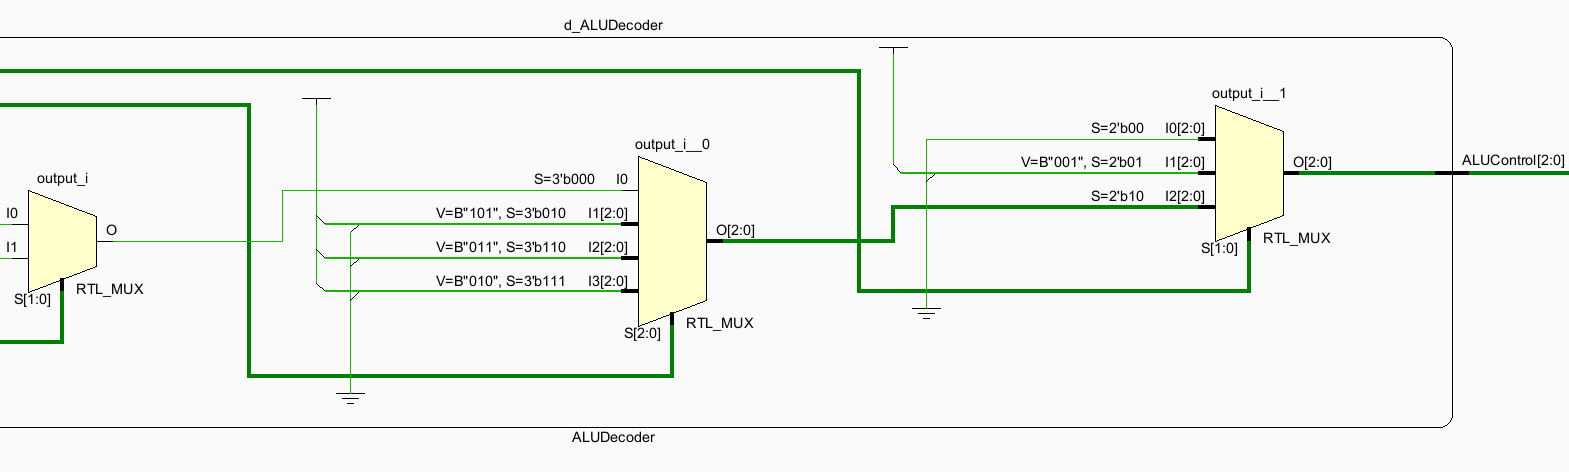
\includegraphics[width=1.0\textwidth]{aludecoder2.png}
 \centering
 \caption{Entitatea VHDL a decodorului aritmetic}
 \label{Figura:47}
 \end{figure}
 
Prin conectarea celor două decodoare, cel aritmetic și cel logic, reuzultă unitatea de decodificare centrală a procesorului. Această entitatea digitală poartă de asemenea numele de unitate de control în cadrul literaturii de specialitate. Figura \ref{Figura:48} prezintă entitatea VHDL aferentă acestei componente.

  \begin{figure}[h!]
 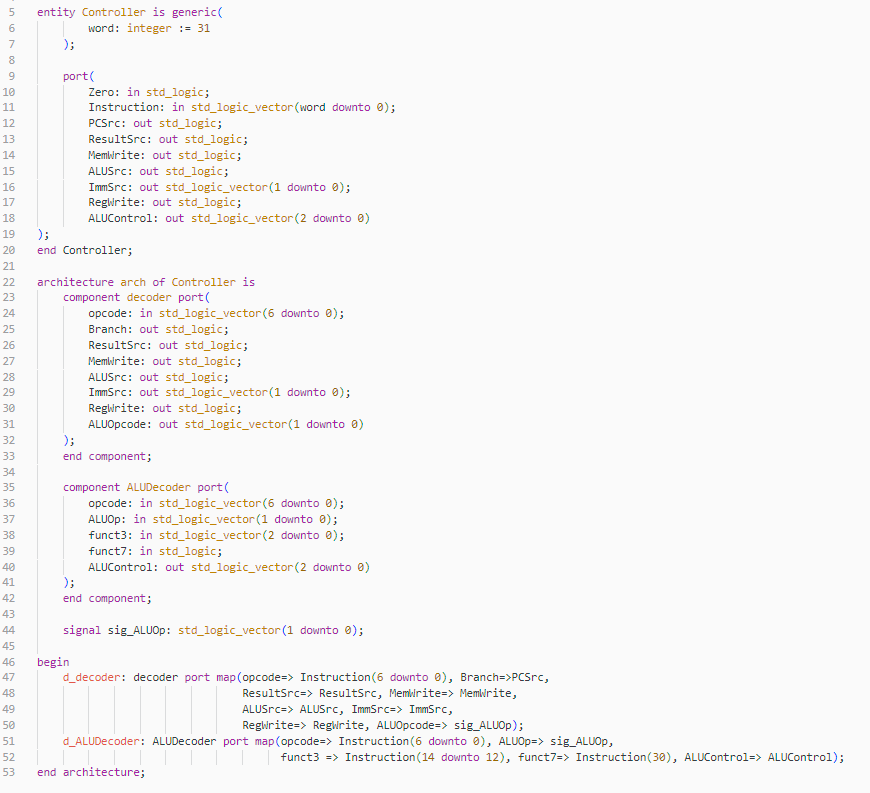
\includegraphics[width=0.8\textwidth]{controllervhdl.png}
 \centering
 \caption{Codul VHDL al entității unității de control}
 \label{Figura:48}
 \end{figure}
 
Circuitul digital generat de sinteză este nimic mai mult decât o interconectare a componentelor anterior menționate, acesta poate fi observat la nivelul Figurii \ref{Figura:49}. 
 
 \begin{figure}[h!]
 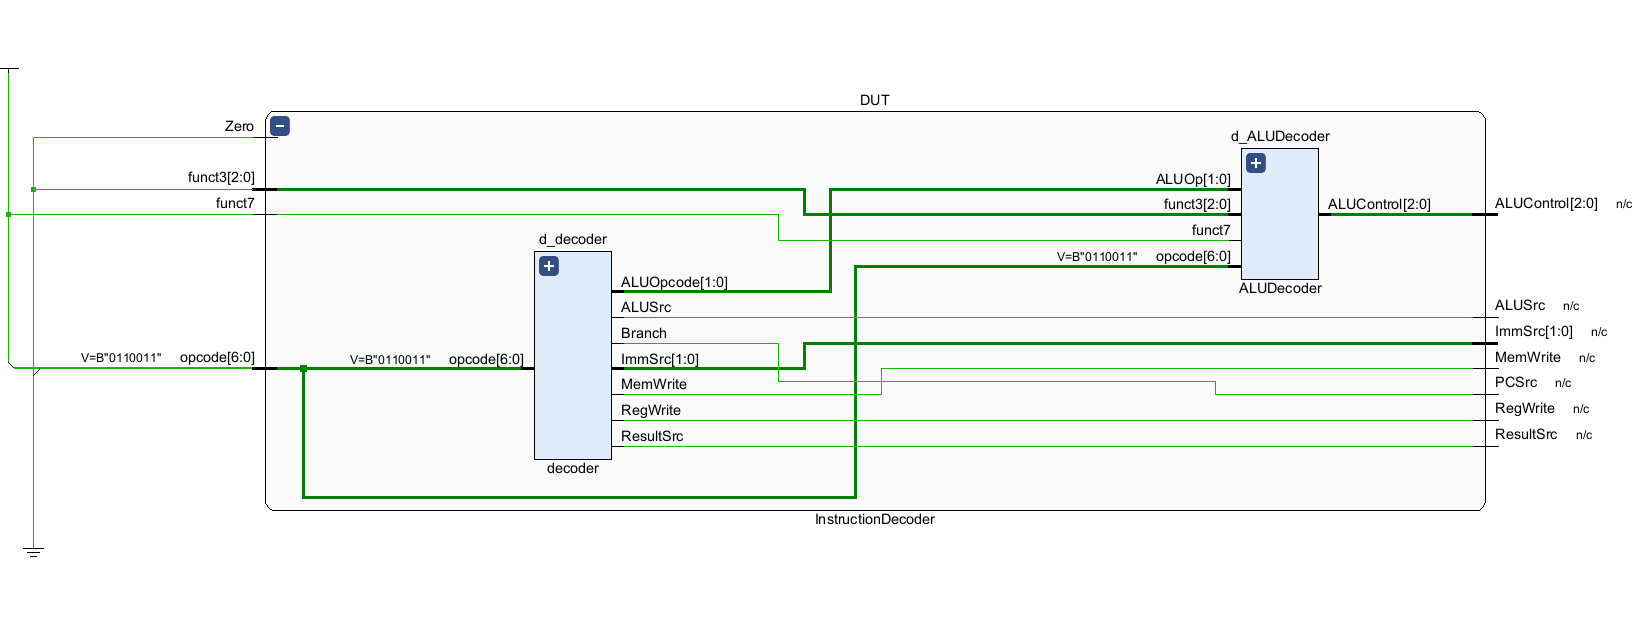
\includegraphics[width=1.05\textwidth]{controller.png}\centering
 \caption{Schema digitală a unității de control}
 \label{Figura:49}
 \end{figure}
 
\subsection{UNITATEA DE EXECUȚIE} 

Unitatea de execuție reprezintă entitatea nucleului procesorului care gestionează calculul aritmetic și logic, dar și calcularea adreselor urmatoarelor instrucțiuni de executat, în funcție de anumite restricții impuse. Restricțiile impuse alegerii subiectului umrătorului ciclu de execuție vin în general sub forma instrucțiunilor de tip branch. 
 
Modelarea acestei componente implică conectarea tuturor entițăților anterior definite, cu excepția unității de control. Un considerent important este faptul că dispozitivele de memorare, mai specific memoriile de instrucțiuni și de date, nu vor fi luate considerate în design-ul unității de control, acestea fiind tratate sub umbrela dispozitivelor externe. Această decizie este luată pentru a crește gradul de modularitate al procesorului, astfel înlăturând limitarea impusă de micile dimensiuni ale unei memorii specifice, existând mereu posibilitatea sporirii mărimi acesteia prin înlocuirea componentei. Mărimea memoriei este unul dintre principalii factori limitatori ai procesoarelor moderne, procesoare care se îndreaptă ușor spre un platou al creșterii vitezei ciclurilor de tact, soluția compensatoare fiind reprezentată de mărimea cache-ului și modificarea arhitecturii interconexiunii cu dispozitivele de memorare către una care eficientizează viteza de acces.

Înainte de a interconecta subcomponentele acestei unități, trebuie definit modul de organizare al execuției, și anume drumul parcurs de datele prevenite din memoria de instrucțiuni, de la operația cerută prin cuvântul de control la calcularea și stocarea rezultatului.

Cea mai vitală conexiune pentru buna funcționare a procesorului este reprezentată de legătura dintre memoria externă de instrucțiuni și program counter-ul. La fiecare ciclu de tact, mai specific pe secvența crescătoare a acestuia, program counter-ul livrează memorii de instrucțiuni index-ul adresei de memorie a căror date sunt destinate procesării.

 Concomitent cu transmiterea unilaterală a datelor, counter-ul incrementează cu 4 octeți index-ul următoarei instrucțiuni de executat. Motivul unei incrementări cu 4 octeți este implementarea arhitecturală byte-addresable a memoriei. Există bineînteles posibilitatea unei incrementări unare, în cazul în care se majorează mărimea datelor din cuprinsul memoriei la mărimea cuvântului cu care lucrează procesorul, în cazul nostru, la 4 octeți. Evident, o astfel de modificare ar însemna o micșorare a spațiului de adresare, adică al numărului de adrese disponibile, la o valoarea egală cu mărimea spațiului de adresare byte-addressable împărțit la numărul de octeți din mărimea adresei refactorizate.
 
 În starea inițială, program counter-ul nu se prezintă ca fiind inițializat cu o valoarea. Inițializarea acestuia implică acționarea pin-ului de reset, încărcându-se astfel în counter valoarea 0. În ciclul de tact următor inițializării, se livrează memoriei de instrucțiuni valoarea prezentă în counter, în cazul nostru 0. Tot în acest ciclu, noua valoare a counter-ului este alesă ca rezultatul multiplexării dintre valoarea incrementată anterior și o nouă valoare calculată, în cazul instrucțiunii beq. Valorile nu sunt încărcate instantaneu datorită naturii secvențiale a acestor componente, ele fiind construite pe baza bistabilelor. Această procedură se repetă până la finalizarea execuției sau până cand adresele din memoria de instrucțiuni sunt epuizate. Figura \ref{Figura:50} prezintă modul în care decurge procedeul descris, acesta reprezentând practic momentul de incepție al execuției.

 \begin{figure}[h!]
 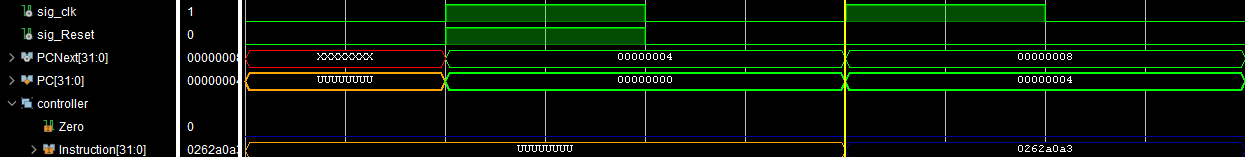
\includegraphics[width=1.025\textwidth]{tbfetch.png}
 \centering
 \caption{Încărcare și incrementarea instrucțiunilor}
 \label{Figura:50}
 \end{figure}
 
 Se observă faptul că înaintea acționării semnalului de reset, \textit{sig rst}, program counter-ul, reprezentat prin semnalul \textit{PC}, este neinițializat, valoarea lui fiiind egală cu \textit{U(Uninitialized)}. Odată ce semnalul de reset este acționat sincron cu semnalul de tact, \textit{sig clk}, program counter-ul este inițializat cu 0. Neexecutându-se o instrucțiune de tip \textit{beq}, valoarea nou calculată pentru counter este egală cu 4, vizibilă la nivelul semnalului \textit{PCNext}.
 
 La următoarea perioadă a ciclului de tact este transmisă valoarea 0 memoriei de instrucțiuni, aceasta transmitând mai departe prin semnalul \textit{Instruction} cuvântul de comandă destinat decodării și execuției. Tot în acest ciclu de tact se modifică valoarea din counter cu cea calculată anterior. Acest procedeu se repetă pentru fiecare instrucțiune de executat. Din punct de vedere digital, circuitul implementat până în acest punct este cel prezentat în Figura \ref{Figura:39}. 

Odată ce adresa instrucțiunii a fost calculată, urmează ca aceasta să fie transmisă unității de control pentru decodarea cuvântului. Concomitent cu decodarea are loc, în funcție de instrucțiune, accesul la nivelul fișierelor de registre, al memoriei și ulterior transmiterea datelor din registrele sau adresele memoriei cerute spre unitatea aritmetică și logică. De asemenea, dacă instrucțiunea are un câmp imediat, se produce cuvântul de calcul prin extensia de semn.
 
Prin urmare, semnalele de intrare ale fișierului de registre destinate accesului vor fi legate la câmpurile de acces al registrelor din cuvântul produs de memoria de instrucțiuni. Semnalul de scriere într-un registru va fi multiplexat între valoarea provenita de la ALU și cea extrasă din memorie, în cazul în care se execută instrucțiunea \textit{lw(load word)}.

 Semnalele de ieșire ale fișierului de registre sunt direct corespondente cu semnalele de intrare ale unității aritmetice și logice. În cazul celui de al doilea operand care se transmite spre ALU,  este însă nevoie de un multiplexor pentru a selecta între valoarea imediată produsă de unitatea extensiei de semn și cuvântul provenit dintr-un registru cerut. Această multiplexare este necesară din cauza nevoii de calcul cu valori imediate, lucru fară de care nu se poate realiza accesul la memoria date.
 
Astfel, diagrama digitală generată de sinteza automată a modului anterior descris de relaționare a componentelor este prezentată în Figura \ref{Figura:51}. Acestă entitate digitală va purta numele de unitatea de execuție a procesorului.

 \begin{figure}[h!]
 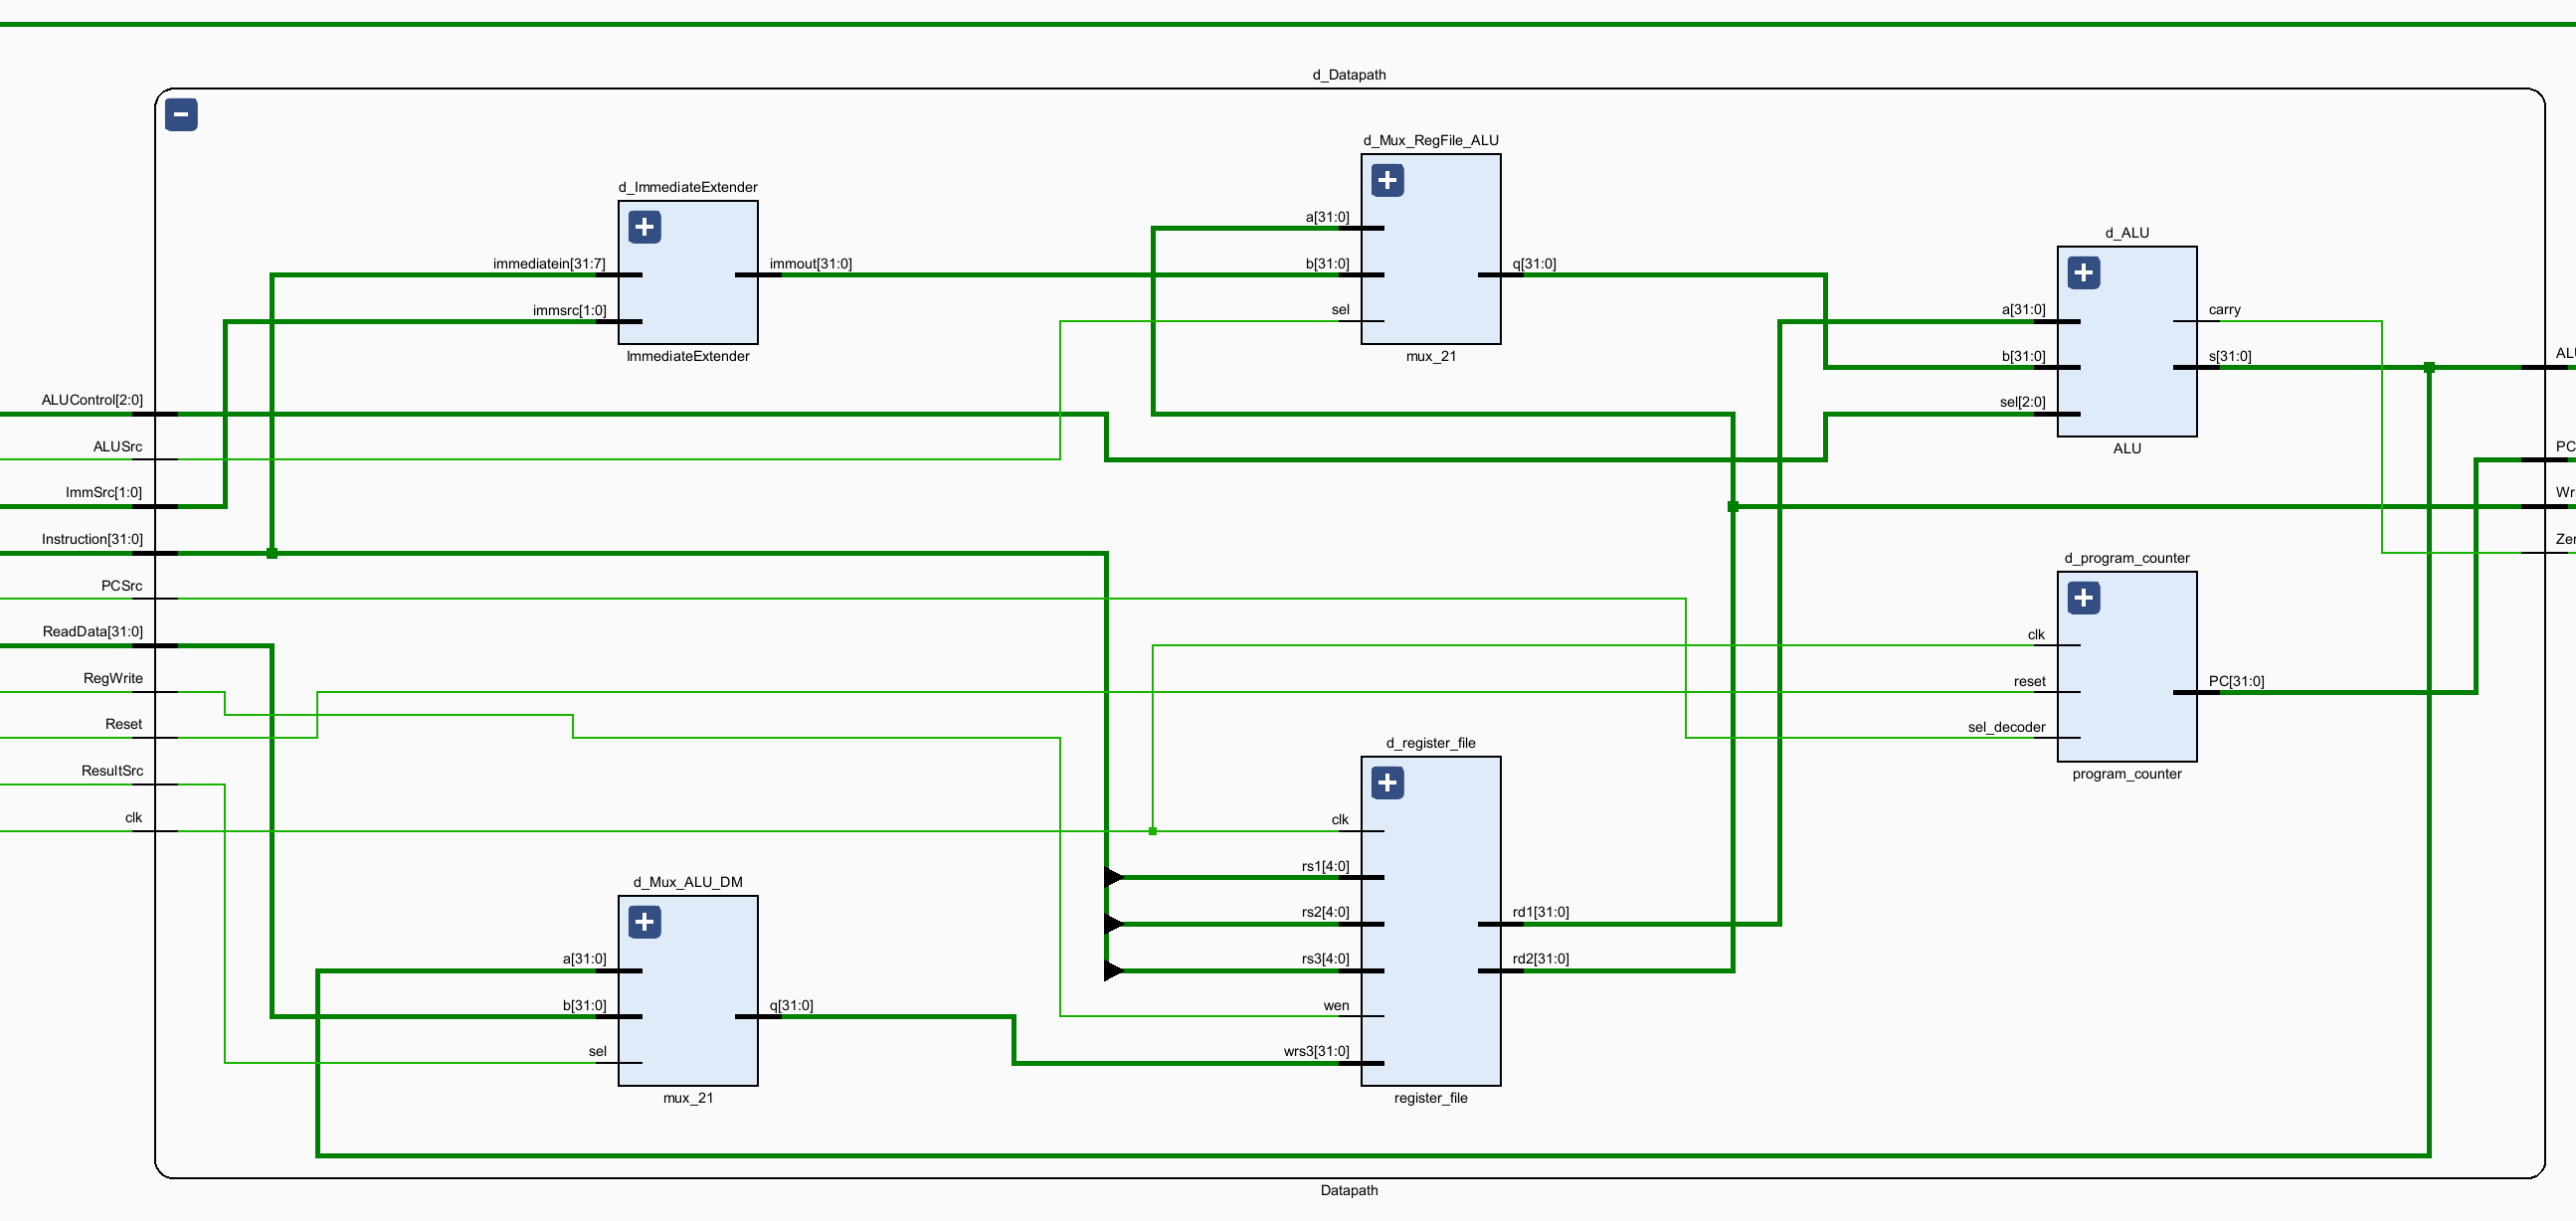
\includegraphics[width=1.0\textwidth]{execunit.png}
 \centering
 \caption{Unitatea de execuție}
 \label{Figura:51}
 \end{figure}
 
Se pot observa clar legăturile dintre componente și rolul operațiilor de multiplexare. De asemenea, sunt vizibile intrările provenite de la unitatea de control, semnalele fiind direcționate fiecărui element cu rol în execuție, sigura excepție fiind program counter-ul. Memoria principală furnizează date prin semnalul  \textit{ReadData}, acesta fiind ulterior multiplexat pentru scriere în registre, în cadrul multiplexorului  \textit{ALU-DM}.

 Semnalele de ieșire sunt reprezentate de datele calculate de ALU, datele provenite din registrul specificat cât și următoarea adresă a instrucțiunii ce urmează a fi executată. Datele provenite din unitatea aritmetică și logică au pentru majoritatea comenzilor un rol intern destinat stocării în registre, dar în cazul instrucțiunilor de tipul \textit{sw(store word)} și \textit{lw(load word)}, acestea au o semnificație externă, indicând adresa de acces la nivelul memoriei de date.
 
\newpage
\subsection{NUCLEUL RISC-V} 
Odata cu modelarea unității de execuție toate componentele microprocesorului sunt finalizate. Prin combinarea unității de control cu cea de execuție rezultă un nucleu RISC-V single-cycle. Termeul de single-cycle provine din faptul că procesorul nostru execută o operație numerică sau de transport a datelor într-o perioadă aproximativ egală cu cea a unui ciclu de tact. Teoretic vorbind, perioada acestui ciclu are ca specificație acoperirea duratei celui mai lung timp de execuție acoperit de una dintre instrucțiunile procesorului. 


Este important de menționat că dispozitivele de memorare nu fac parte din nucleul propriu-zis, memoria fiind considerată o entitate modulară și mutabilă. Figura \ref{Figura:52} prezintă nucleul RISC-V generat de sinteza automată. Alături de cele 2 unități structurale se poate observa prezența memoriei de date și a celei de instrucțiuni.

 \begin{figure}[h!]
 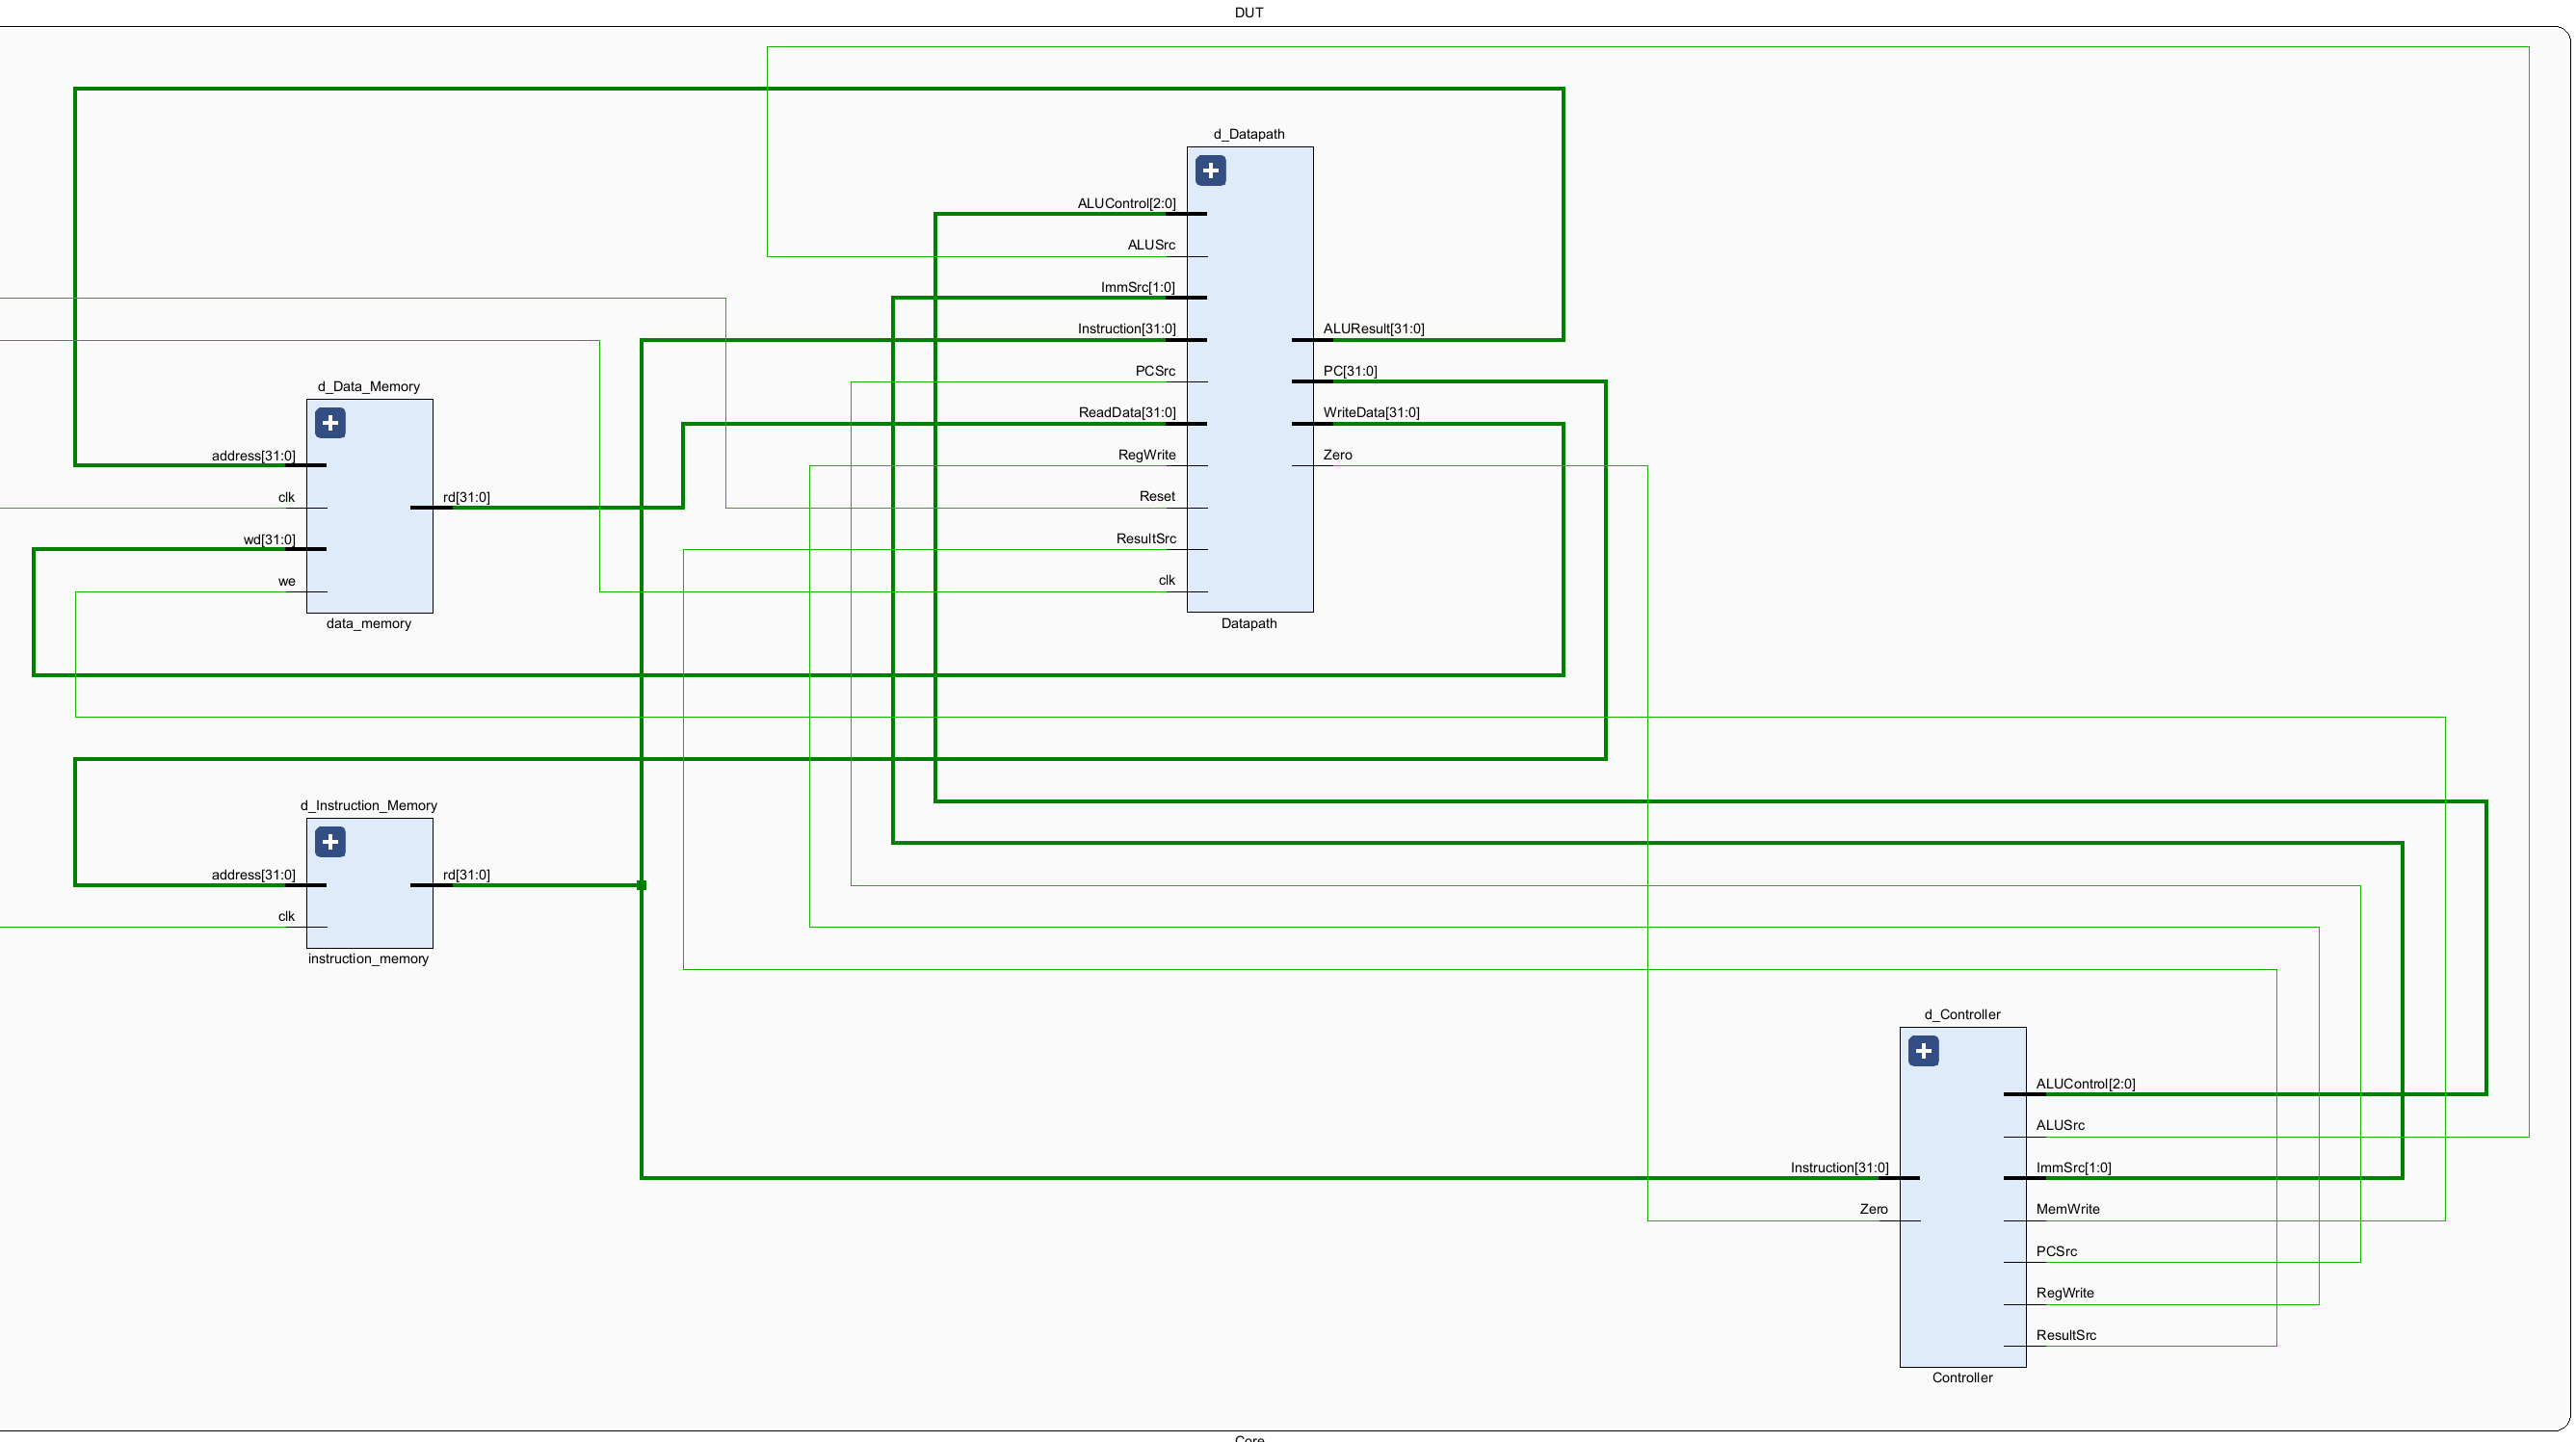
\includegraphics[width=1.0\textwidth]{core.png}
 \centering
 \caption{Nucleul RISC-V RV32I}
 \label{Figura:52}
 \end{figure}


Entitatea VHDL a nucleului este formată în jururul tuturor entităților superioare implementate. Semnalele de comunicare între componentele microprocesorului sunt de o importanță deosebită, acestea fiind practic impulsurile care asigură funcționarea corectă a tuturor modulelor odată cu execuția unei instrucțiuni. O legare inadecvată implică activarea unei suite de module hardware greșite, rezultatul calculelor fiind astfel irelevant și incorect.
 
De asemenea, semnalele trebuie inițializate prevenind astfel intrarea pe ramuri de execuție încă nedefinite. Spre exemplu, o valoare inițială alta decât 0 poate activa dispozitivele de memorare, scriind astfel date aleatorii la adrese nedestinate scrierii.

Codul sursă VHDL aferent nucleului se regăsește la nivelul Figurii \ref{Figura:53}.
\newpage
  \begin{figure}[h!]
 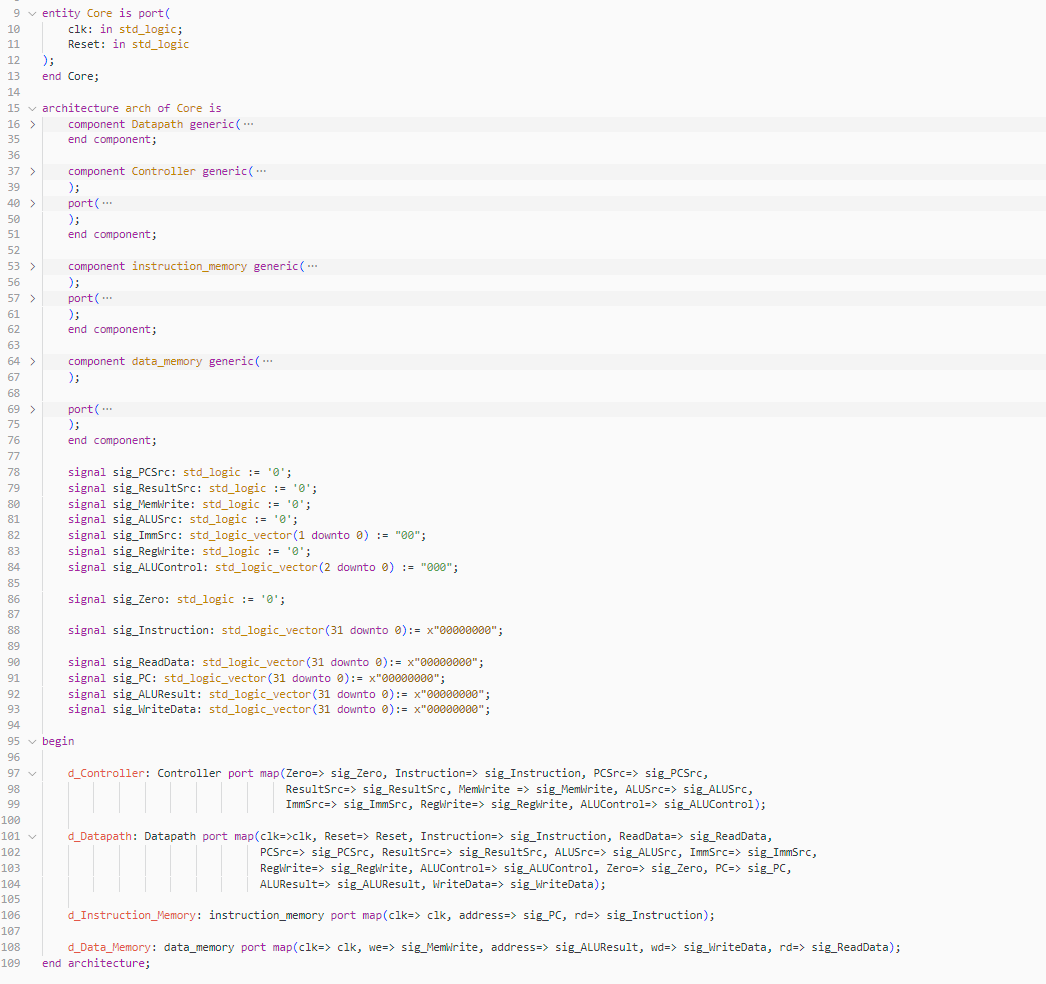
\includegraphics[width=1.0\textwidth]{riscvcore.png}
 \centering
 \caption{Nucleul RISC-V ca entitate VHDL}
 \label{Figura:53}
 \end{figure}
 
 
Procesorul single-cycle are ca mare avantaj relativa simplitate a implementării digitale.  Dezavantajul unui astfel de procesor este faptul că suntem limitați din punct de vedere al operațiilor pe care le putem executa. Comenzi complexe asupa numerelor precum înmulțirea și împărțirea nu sunt astfel fezabile, alternativa reprezentării acestora fiind adunări, scăderi și aproximări repetate.

 În ciuda acestor probleme, procesorul single-cycle este o implementare cu un caracter didactic valoros, existând posibilitatea extinderii sale într-o unitate de execuție multi-cycle cu vaste capabilități și aplicații.
 
\newpage
\subsection{MEMORIA CACHE}

În cazul în care dorim utilizarea unei memorii de date cu latență ridicată a accesului la date, utilizarea unei memorii cache intermediare devine obligatorie în creșterea metricilor de execuție. Astfel, ca posibilă soluție de implementare, se va prezenta procesul de design al unei memorii cache pe decursul acestui capitol. Ca mențiune, cache-ul este de-a dreptul opțional pentru buna funcționare a nucleului singe-cycle, acesta fiind dezvoltat în jurul unor memorii de date și instrucțiuni construite pe baza matricilor de registre.
 
Precum dictează intuiția, sunt 2 utilizări spre care ne putem îndrepta când vine vorba de folosirea cache-ului în cardul unui sistem de calcul. Primul drum este marcat de utilizarea clasică care implică extragerea blocurilor de date din memoria principală, eliminând latența de acces. A doua cale este marcată de utilizarea cache-ului cu scop în minimizarea latenței de transmitere a instrucțiunilor ce urmează rulate.

Aceste 2 metodologii nu trebuie însă tratate ca fiind mutual exclusive, ambele fiind implementate la nivelul unui procesor, reprezentând un mare salt făcut spre maximizarea randamentului computațional.

Design-ul unui cache începe cu memoriile \textit{CACHE SRAM} și \textit{TAG SRAM}, urmând ca schimbul acestora cu memoria inferioară să fie orchestrat de un \textit{cache controler}.

Pentru simplificarea ilustrării conceptelor de design, se va lua în considerare că procesorul, pentru care implementăm acest nivel de cache, are o arhitectura pe 8 biți și un spațiu de adresare al memoriei egal cu $\ 2^{16}$ adrese byte-addresable. Practic, cuvântul de lucru al microprocesorului de 1 octet este congruent cu octetul dintr-o adresa.

Pentru a determina modul în care biții din adresă sunt împărțiti este nevoie prima dată de definirea mărimii memoriei cache cât și a blocurilor care o compun. Pentru simplificarea calculelor, cache-ul va fi compus din 8 blocuri, fiecare bloc având un număr de 4 octeți. 

Prin urmare, câmpului de offset îi vor fi alocați $\  log_2 4 = 2 $ biți, urmând ca câmpul index sa fie compus din$\  log_2 8 = 3 $ biți. Restul de 11 biți vor fi reprezentați de identificatorul unic asociat unei serii de 8 seturi, și anume tag-ul. în Figura \ref{Figura:54} se poate vedea clar acest aranjament.

 \begin{figure}[h!]
 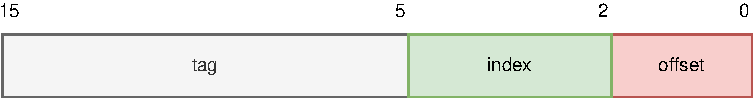
\includegraphics[width=0.8\textwidth]{cache16bit.pdf}
 \centering
 \caption{Câmpurile din adresa memoriei}
 \label{Figura:54}
 \end{figure}

Memoria cache SRAM are ca structura diagrama digitală din Figura \ref{Figura:55}. Se pot distinge cele 8 registre cu o mărime de 32 de biți care sunt ulterior trecute printr-o serie de 8 buffere urmând ca semnalul de ieșire sa fie ales de multiplexor conform semnalului de selecție controlat de index-ul blocului relevant.

 \newpage
 \begin{figure}[h!]
 \includegraphics[width=0.82\textwidth]{cachesram.png}
 \centering
 \caption{Structura memorie cache SRAM}
 \label{Figura:55}
 \end{figure}
 
 Codul din spatele acestei generări este prezentat în Figura  \ref{Figura:56}.
  \begin{figure}[h!]
 \includegraphics[width=0.6\textwidth]{cachesramcode.png}
 \centering
 \caption{Codul VHDL aferent memorie cache SRAM}
 \label{Figura:56}
 \end{figure}

În ceea ce privește tag-ul, acesta va fi stocat în memoria tag SRAM a cărei structură este similara cu cea a cache SRAM-ului. Pe lânge câmpul de 10 biți ce reprezintă tag-ul, se mai folosește un bit de validitate, acesta fiind pus pe 1 odată cu aducerea unui bloc in cache. Semnalele de intrare ale acestei componente sunt reprezenta de comanda de citire, prin semnalul \textit{read tag} și de comanda de scriere, prin \textit{write tag}.

Structura memoriei tag SRAM este relatată la nivel digital în Figura \ref{Figura:57}.

  \begin{figure}[h!]
 \includegraphics[angle=-90,width=0.71\textwidth]{tagsram.png}
 \centering
 \caption{Diagrama digitală a memoriei tag SRAM}
 \label{Figura:57}
 \end{figure}
 
Prima jumătate a structurii este similară cu cea a cache SRAM-ului, fiind compusă din registre si elemente de buffer pentru procedura de multiplexare după index. Diferența vine sub forma circuitului de selecție al semnalului de ieșire, acesta fiind condiționat de cele 2 intrări. Prin urmare, semnalul de ieșire este reprezentat de tag-ul de interes. Prezența unui tag valid semnifică existența unui bloc de cache din memoria principală, lipsa tag-ului arată viceversa. Codul acestei implementări se regăsește la nivelul Figurii \ref{Figura:58}.

  \begin{figure}[h!]
 \includegraphics[width=0.9\textwidth]{tagsramvhdl.png}
 \centering
 \caption{Diagrama digitală a memoriei tag SRAM}
 \label{Figura:58}
 \end{figure}
  
\newpage 
\section{\centering BIBLIOGRAFIE}
\begin{thebibliography}{0}

\bibitem{riscv}
Sarah Harris, David Harris (Octombrie, 2021), Digital Design and Computer Architecture, RISC-V Edition: RISC-V Edition, Morgan Kaufmann.
\bibitem{code}
Charles Petzold (Octombrie, 2000), Code: The Hidden Language of Computer Hardware and Software, Microsoft Press.
\bibitem{roscv_petterson}
David A. Patterson, John L. Hennessy (Aprilie, 2017), omputer Organization and Design RISC-V Edition: The Hardware Software Interface, Morgan Kaufmann.

\end{thebibliography}
\end{document}






La nivelul fișierului de registre nu se efectuează nimic altceva decât citirea datelor din registrele \textit{rs1, rs2}, urmând ca informația din \textit{rs1} să fie transmisă memoriei pentru scriere. Datele din registrul \textit{rs2} sunt folosite pentru calculul adresei cu un offset livrat prin câmpul imediat al instrucțiuni, acesta fiind în prealabil extins la 4 octeți.

Primul lucru pe care-l vom analiza este modul în care unitatea de control efectuează decodarea cuvintelor de comandă, acesta fiind prezentat în Figura \ref{Figura:51}.

 \begin{figure}[h!]
 \centering
 \caption{Decodarea instrucțiunii}
 \label{Figura:51}
 \includegraphics[width=1.0\textwidth]{tbdecoding.png}
 \end{figure}
 
Instrucțiunea primită fiind una de acces la nivelul memoriei, se poate observa setarea pe 1 logic a semnalului care comandă acest lucru, și anume \textit{MemWrite}. Cuvântul transmis subunității de calcul aritmetic este cel decodat în efectuarea operației de însumare de către aceasta. Însumarea are loc datorită modului de calcul cu offset al adresei de scriere, precum se specifică de arhitectura RISC-V. Pentru o vedere detaliată asupra modului în care această decodare se efectuează, se recomandă consultarea Tabelei \ref{Tabela:16} și respectiv a Tabelei \ref{Tabela:17}.